\chapter{HiSPARC Station 14008}\label{chap:HiSPARC_14008}

%%%%%%%%%%%%%%%%%%%%%%%%%%%%%%%%%%%%%%%%%%%%%%%%%%%%%%%%%%%%%%%%%%%%%
%%%%%%%%%%%%%%%%%%%%%%%%%%%%%%%%%%%%%%%%%%%%%%%%%%%%%%%%%%%%%%%%%%%%%
\section{Introduction}\label{sec:HS_14008_intro}


%... [on daily variations (DV)] Dr. Rolf Butikofer (in a reply from Danislav Sapundjiev, dasapund@meteo.be) said:
%
%\textit{"The daily cosmic ray variation near Earth is caused by the anisotropy of the cosmic ray intensity in the interplanetary space. Cosmic ray particles follow the field lines of the interplanetary magnetic field when they travel towards the interior of the heliosphere. Because of the rotation of the Earth, the angle between the asymptotic cone of acceptance of various energies at the location of ground-based cosmic ray detectors (neutron monitors) and the direction of the interplanetary magnetic field varies with a time period of 24 hours. As a consequence cosmic ray detectors look in different directions in the course of a day and observe therefore a diurnal variation. The daily variations of neutron monitors is mainly seen by high latitude stations which have asymptotic directions at low energies (rigidities) near the equator."}



It was shown in Chapter~\ref{chap:HiSPARC}, using data acquired by the \gls{hisparc} network, that in its original configuration, \gls{hisparc} was not adequate for observing space weather events. In part, we showed that this was due to the low-magnitude of the increase in the expected muon flux during such events. Also relevant was the current configuration's bias towards higher energy \glspl{cr} and the sensitivity of the detectors to variations in meteorological conditions.

To some extent, it was possible to eliminate the variation in \glspl{cr} due to meteorological variations in the \gls{hisparc} data; however, it was shown to not always be effective, as different detectors in the \gls{hisparc} network displayed different responses to pressure and temperature variation and the correlation between atmospheric temperature and \gls{cr} count was weaker than the counterpart for pressure.

Thermal fluctuations in the atmosphere induce thermal noise in the \glspl{pmt} and although the temperature inside the \gls{hisparc} roof boxes has not been measured, it is suspected that the \glspl{pmt} can get quite hot, in particular when the roof boxes are in direct sunlight. We reported in Chapter~\ref{chap:HiSPARC} that the singles data represented our best possibility of observing lower-energy \glspl{pcr}; however, these data are most susceptible to the induced thermal noise as the temperature of the \gls{pmt} changes. Without measuring this temperature directly, a complete correction of this effect in the existing \gls{hisparc} data was not possible.

In this chapter we describe an alternative configuration of \gls{hisparc} station, which was devised and tested, to minimise these limiting effects. An instance of thermal noise in a single \gls{pmt} will be random, and uncorrelated with an instance of thermal noise in another \gls{pmt}. To exploit this, we stacked two detectors on top of each other and put them in coincidence to measure a single muon which traverses both scintillators, hence inducing signals in both \glspl{pmt}.




%%%%%%%%%%%%%%%%%%%%%%%%%%%%%%%%%%%%%%%%%%%%%%%%%%%%%%%%%%%%%%%%%%%%%
%%%%%%%%%%%%%%%%%%%%%%%%%%%%%%%%%%%%%%%%%%%%%%%%%%%%%%%%%%%%%%%%%%%%%
\section{Aims}\label{sec:HS_14008_aims}

The principal aim of building a new \gls{hisparc} station was to investigate whether an alternative configuration of a \gls{hisparc} station could minimise atmospheric variations in the data. In addition, we aimed to demonstrate a configuration that allowed for the observation of space weather events.

We aimed to set up a new detector, perform the relevant atmospheric corrections, where necessary, and review the noise properties of the detector. Furthermore, we also aimed to perform simulations of \glspl{gle} of varying physical properties to understand what magnitude of \gls{gle} could be observed with the new set-up. This would help us to understand how likely it was to observe the any space weather events with the alternative \gls{hisparc} station configuration.



%%%%%%%%%%%%%%%%%%%%%%%%%%%%%%%%%%%%%%%%%%%%%%%%%%%%%%%%%%%%%%%%%%%%%
%%%%%%%%%%%%%%%%%%%%%%%%%%%%%%%%%%%%%%%%%%%%%%%%%%%%%%%%%%%%%%%%%%%%%
\section{HiSPARC Station 14008 Set-Up}\label{sec:HiSPARC_14008}


%%%%%%%%%%%%%%%%%%%%%%%%%%%%%%%%%%%%%%%%%%%%%%%%%%%%%%%%%%%%%%%%%%%%%
\subsection{Configuration}

The new configuration, of \gls{hisparc} station 14008, is shown in Figure~\ref{fig:14008_config}; it is composed of two detectors stacked on top of each other, both inside one roof box, and the signals from the \glspl{pmt} are put in coincidence. This configuration is advantageous over the single-scintillator, single-\gls{pmt} \gls{hisparc} set-up, as it allows the measurement of single muons that traverse both scintillators. 


\begin{figure}[ht!]
	\center
	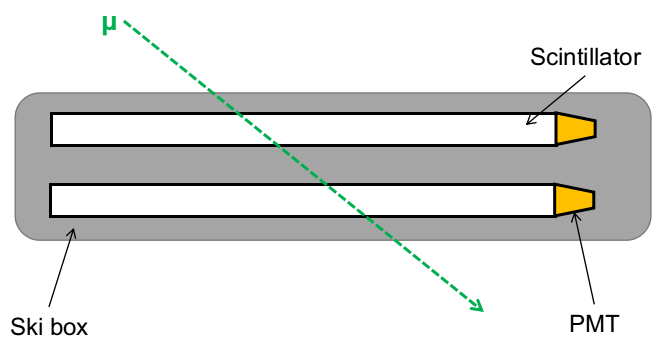
\includegraphics[width=0.75\columnwidth]{14008_config.png}
	\caption{Schematic diagram of the HiSPARC station 14008 detector set-up within the roof box.}
	\label{fig:14008_config}
\end{figure}

We showed in Chapter~\ref{chap:HiSPARC} that the existing \gls{hisparc} design, requiring coincident triggers between detectors spaced tens of metres apart, biased the observations to higher \gls{pcr} energies and single muons from lower energy \glspl{pcr} could not be counted. Previously, we could only count single muons in the singles rates, but we have shown that the data were inconsistent between stations and it was difficult to disentangle the effects of temperature, \gls{pmt} noise, and the diurnal effect in the data. This stacked-configuration design reduces the energy bias in the events data, as it no longer requires the large footprint \glspl{as} to trigger multiple detectors, and provides a signal with fewer sources of noise than the singles rates, as it relies on the coincidence of two \glspl{pmt} therefore minimising thermal fluctuations.

To protect the scintillators and \glspl{pmt}, we sandwiched a layer of high density ($\rho = 38-40$~kg~m$^{-3}$, \citet{efoam_sf38_2017}) foam, of thickness $\Delta x = 50$~mm, between the scintillators, as can be in Figure~\ref{fig:14008_config} and Figure~\ref{fig:14008_detectors}. Upon the completed assembly of the detectors, they were placed within the roof box on the roof of the Poynting Physics building on the University of Birmingham campus (see Fig.~\ref{fig:HS_14008_setup}).


\begin{figure}[ht!]
	\centering
	\subfloat[Scintillators inside roof box]{
		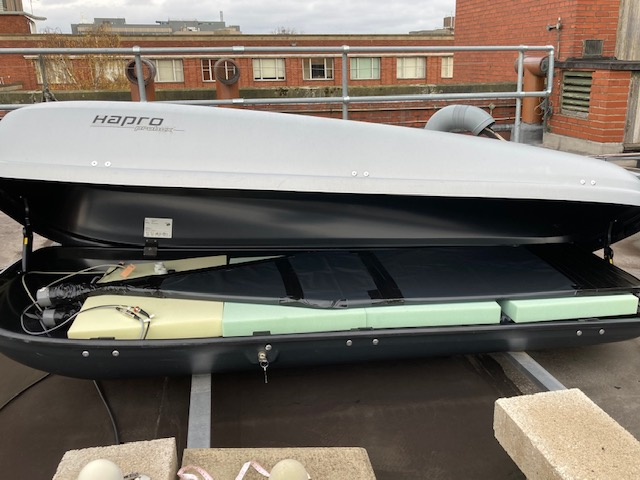
\includegraphics[width=0.48\columnwidth]{detectors_in_box.jpg}
		\label{fig:14008_detectors}}
	%\qquad
	\subfloat[Complete detector on the roof]{
		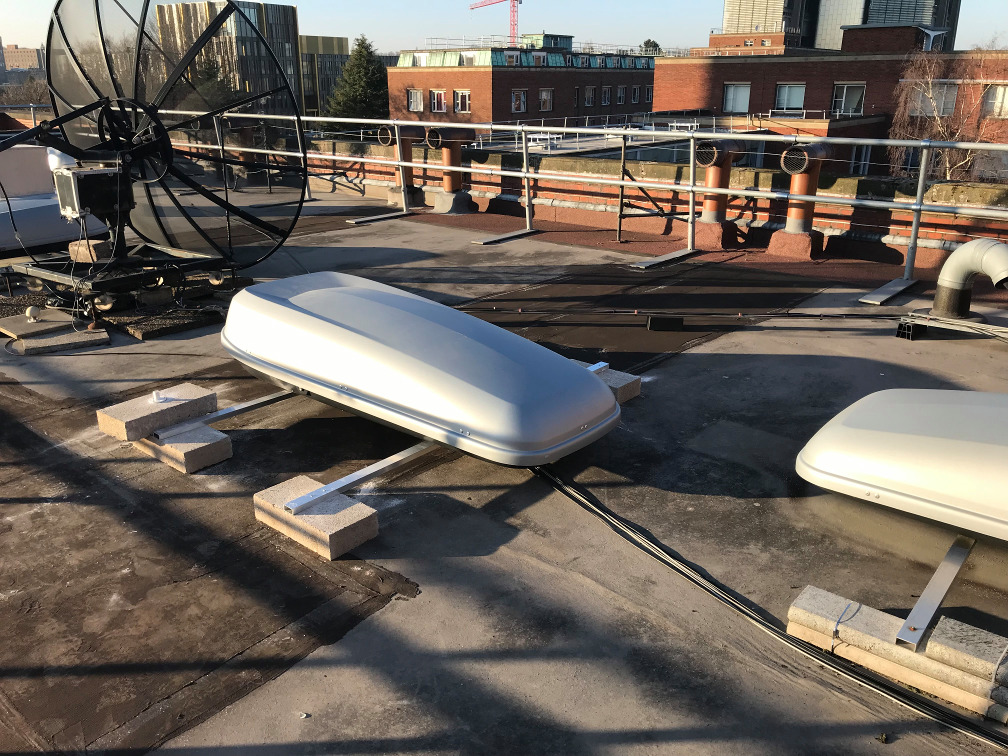
\includegraphics[width=0.48\columnwidth]{ski_box_rescaled.jpg}
		\label{fig:14008_ski_box}} \\
	
	\caption{HiSPARC 14008 assembly and configuration. (a) Shows the stacked arrangement of the scintillators within the roof box, between layers of protective foam. (b) Shows the complete detector on the roof of the Poynting building on the University of Birmingham campus.}
	\label{fig:HS_14008_setup}
\end{figure}


Propagating charged particles lose energy in matter. Derived from the Bethe-Bloch formula \citep{bethe_bremsformel_1932, ziegler_stopping_1999}; we can estimate the amount of energy lost by a particle in a material as:
%
\begin{equation}
\Delta E = \Delta x \, S \, \rho \, \cos(\theta) \, ,
\label{eq:energy_loss}
\end{equation}
%
where $\Delta x$ is the thickness of the material, $S$ is the stopping power of the material, $\rho$ is the density of the material, and $\theta$ is the angle the particle travels through the material from the perpendicular direction.

Each of the plastic scintillators has a thickness of $\Delta x \, = \, 2.0$~cm, and density, $\rho \, = \, 1.03$~g~cm$^{-3}$ \citep{montanus_observability_2017}. The stopping power of the scintillator for a minimum ionising particle is $S \sim 2$~MeV~g$^{-1}$~cm$^{2}$ \citep{fokkema_hisparc_2012, montanus_observability_2017}. The energy loss of a vertically incident muon in a single detector is therefore $\Delta E \sim 4$~MeV. \cite{van_dam_hisparc_2020} states the most probable energy loss of a vertically incident muon in a single scintillator is approximately $3.51$~MeV.

Assuming a similar stopping power as above for the foam \citep{groom_muon_2001, montanus_observability_2017}, the muons will lose an additional $\sim 0.4$~MeV. In the complete configuration, as a muon traverses two scintillators and the foam, the estimated lower limit on the energy loss by muons in the detector is $\sim 7.4$~MeV. This new lower limit does not significantly change the values of the predicted \gls{gle} magnitudes in Section~\ref{sec:MAIRE_flux}.

The standard \gls{hisparc} station set-up is such that the \glspl{pmt} are connected to the \gls{hisparc} electronics box for data acquisition. In the standard \gls{hisparc} station configuration, the trigger rate of events is $\sim$1~Hz. In this stacked configuration the trigger rate is significantly higher, $\sim$80~Hz; hence the data produced is the equivalent of approximately half of the existing \gls{hisparc} network. The \gls{hisparc} servers could not cope with such a large quantity of data, therefore we had to reduce the data acquired by the \gls{hisparc} box; however, we did not want to lose the original count rate of the stacked detectors. To acquire the data in this set-up, we used a \gls{nim} crate, as shown in Figure~\ref{fig:14008_NIM}, and a Raspberry Pi was used to store the data, which is discussed in Section~\ref{sec:HS14008_data_acqusition}.

\begin{figure}[ht!]
	\centering
	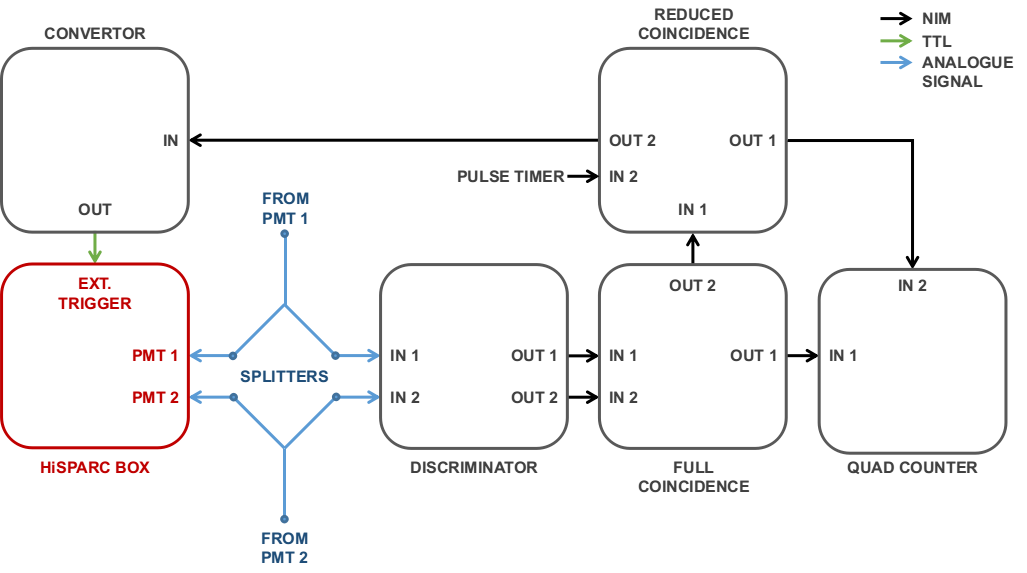
\includegraphics[width=\columnwidth]{14008_nim_config.png}
	\caption{Schematic diagram of the HiSPARC 14008 station NIM crate configuration. Black-outlined boxes indicate the NIM crate modules, while red-outlined boxes depict HiSPARC hardware modules. Black arrows depict a NIM signal; green arrows show a TTL signal; blue arrows depict the analogue signal from the PMTs. The PMT signals are split and half of the signal interfaces directly with the HiSPARC electronics box and half the signal is passed through the NIM crate for processing.}
	\label{fig:14008_NIM}
\end{figure}

The data acquisition is discussed in Section~\ref{sec:HS14008_data_acqusition}, but here we discuss the configuration of the \gls{nim} crate set-up. The analogue signals from the \glspl{pmt} are split using a passive, equal-split resistive splitter such that half the signal is passed to the \gls{hisparc} electronics box and half the signal is passed through the \gls{nim} crate. The analogue signal which is passed through the \gls{nim} crate goes first into a discriminator module (CAEN model N845) to only record signals that have an amplitude greater than the trigger threshold. Due to the equal-balance resistive splitter the \gls{pmt} signal is reduced in amplitude by a factor of 2; we used a discriminator threshold of $-35$~mV, i.e. half of the \gls{hisparc} high threshold.
% SPLITTER: Zin = Z0 = R +(R+Z0)/2 --> R1 = Z0/3

The discriminator outputs two \gls{nim} signals which are connected to the first coincidence module (LeCroy model 622). This records every coincidence between the two \glspl{pmt} and the output from this module is directed to a \gls{nim} quad counter/timer module (ORTEC model 974). One channel of the \gls{nim} counter records the original coincidence counts from the first coincidence module.

A second terminal in the coincidence module was used to record a reduced count rate. This used a pulse timer (CAEN model 2255B) to create a gate signal with a duty cycle of $\sim 1\%$ (gate width = $45.0 \, \upmu\mathrm{s}$; period = $4.86$~ms). The coincidence between the original coincidence signal and the pulse timer gate ensures that the original count rate is reduced by a factor of $\sim$100. This was a sufficient reduction in the data for the \gls{hisparc} servers to cope with. One output from this coincidence module is passed to the \gls{nim} counter, where it counts the reduced coincidences. The second output from the coincidence module is directed through a \gls{nim}-to-\gls{ttl} converter and the output from this is used as an external trigger signal for the acquisition of data by the \gls{hisparc} electronics box. This trigger was used to acquire the counts directly from the \glspl{pmt} in the normal \gls{hisparc} manner.%, but with a reduced frequency by a factor of $\sim100$.

The use of these \gls{nim} modules introduces delays in the signal. Each of the \gls{nim} modules introduces a \gls{nim}-standard, typical input-output delay of $\sim$9.5~ns \citep{lecroy_lecroy_1996, caen_technical_2011}. In Table~\ref{tab:HS_14008_delays} we outline the delays that are introduced from the outputs of the \glspl{pmt} to being registered at different end-points.

\vspace{1em}

\begin{table}[ht!]
	\begin{center}
		\caption{Delays in the signals through different paths in the NIM set-up. The paths all start from the output of the PMTs, and are either direct or pass though the NIM crate before reaching their final end interface, therefore the path column is formatted as: start -- direct/NIM path -- end.}
		\label{tab:HS_14008_delays}
		\begin{tabular}{l c }
			\hline 
			{\bf Path} & {\bf Delay [ns]} \\ 
			\hline 
			PMT -- direct -- HiSPARC Box &  16 \\ 
			PMT -- NIM -- Ext. Trigger HiSPARC Box & 52 \\ 
			PMT -- NIM -- Counter (Reduced) & 37 \\ 
			PMT -- NIM -- Counter (Full) & 29 \\ 
			\hline 
		\end{tabular} 
	\end{center}
\end{table}

%\begin{table}[ht!]
%	\begin{center}
%		\caption{... NIM crate delays...}
%		\label{tab:HS_14008_nim_delays}
%		\begin{tabular}{l c }
%			\hline 
%			{\bf NIM Module} & {\bf I/O Delay [ns]} \\ 
%			\hline 
%			CAEN N845 &  9.5 \\ 
%			LeCroy 622 & 9.5 \\ 
%			ORTEC 974 & 9.5 \\ %but this delay doesn't count in the combined delays as we don't wait for it!
%			\hline 
%		\end{tabular} 
%	\end{center}
%\end{table}

From Table~\ref{tab:HS_14008_delays} we see there is a delay of $\sim36$~ns between the direct signal to the \gls{hisparc} electronics box and the external trigger from the \gls{nim} crate. There is also an $\sim8$~ns delay in between the full count and the reduced count. However, the delays introduced into the system are not actually a problem for counting muons with the \gls{hisparc} electronics box or the \gls{nim} counter. In the case of the \gls{hisparc} electronics box the effect of the delays is mitigated by the low muon count rate and the wide pre- and post-trigger windows of the \gls{hisparc} data acquisition software (discussed in Section~\ref{sec:intro_HS_DAQ}). The \gls{hisparc} data acquisition software uses pre-trigger ($1\,\upmu\mathrm{s}$), coincidence ($1.5\,\upmu\mathrm{s}$) and post-trigger ($3.5\,\upmu\mathrm{s}$) windows \citep{fokkema_hisparc_2012}. This means that the signals coming from our \gls{nim} setup, with a maximum delay of less than 60~ns, will be easily captured within the $1\,\upmu\mathrm{s}$ pre-trigger window and thus counted. Using the \gls{nim} counter, as discussed in Section~\ref{sec:HS14008_data_acqusition}, we measure all counts in time intervals of 10-seconds, therefore a delay of $\sim$8~ns does not impede our ability to count the events during the cadences.


%%%%%%%%%%%%%%%%%%%%%%%%%%%%%%%%%%%%%%%%%%%%%%%%%%%%%%%%%%%%%%%%%%%%%
\subsection{Calibration}

When setting up the HiSPARC station, it was required to set several operating parameters for the detectors and the HiSPARC electronics box. One such setting was the \gls{pmt} operating \gls{hv}. Each of the detector \glspl{pmt} needs to be powered with a high enough operating voltage to provide an amplified signal, but not too high such as to over-amplify the noise.

In general, the \glspl{pmt} have an advised operating voltage of around 700~V \citep{fokkema_hisparc_2019}; however, best practise is to operate the \gls{pmt} at the plateau region, whereby the counts/voltage no longer increases. As can be seen from Figure~\ref{fig:PMT_cal}, neither of the \glspl{pmt} have clear plateau regions, hence there was no obvious \gls{pmt} set point.

The HiSPARC installation manual does, however, suggest to tune the \gls{pmt} voltages such that the singles rates for each detector meet the following criteria: singles rate of 100--130~Hz for signal above the high trigger threshold, and singles rate of $<$400~Hz for signal above the low trigger threshold \citep{fokkema_hisparc_2019}.

In order to calibrate the \glspl{pmt} to the correct level, we measured the singles rates above the high and low thresholds as a function of \gls{pmt} operating voltage, as is shown in Figure~\ref{fig:PMT_cal}. The \gls{hv} calibration plot shows the different performances one can get from different \glspl{pmt}, therefore it was necessary to treat each \gls{pmt} individually when calibrating.

\begin{figure}[ht!]
	\centering
	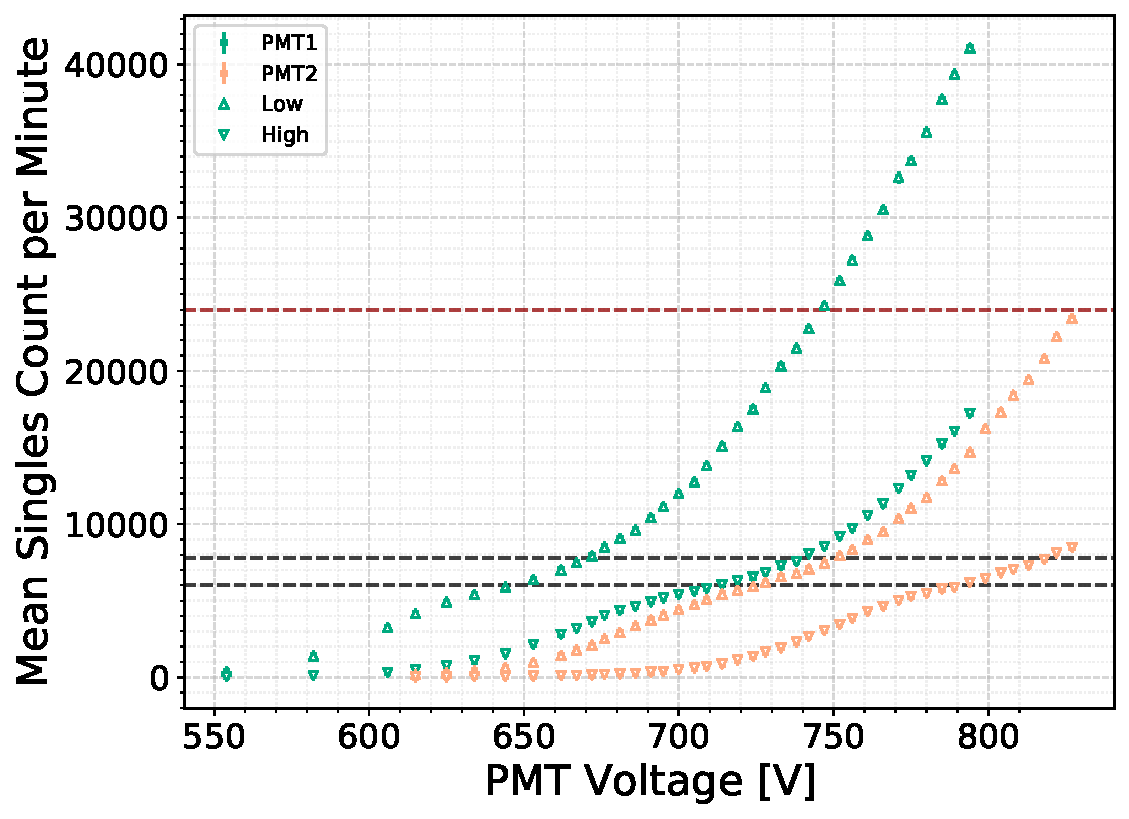
\includegraphics[width=0.8\columnwidth]{both_PMTs_post_NIM.pdf}
	\caption{Voltage calibration curve for the PMTs of station 14008. The upper, red-dashed line indicates the upper limit for the low threshold singles rate (400 Hz), and the lower 2, black-dashed lines indicate the upper and lower bounds for the high threshold singles rate (100--130 Hz).}
	\label{fig:PMT_cal}
\end{figure}

Initially the station was set-up supplying \gls{pmt}1 and \gls{pmt}2 $\sim$725~V and $\sim$790~V, respectively, based on the calibration in Figure~\ref{fig:PMT_cal}. However, after some time the rates had drifted, perhaps due to early life-time variations in the \gls{pmt} operations. After a re-calibration, since the end of 2019 the station has been consistently operating with \gls{pmt}1 and \gls{pmt}2 voltages of $725$~V and $851$~V, respectively.




%%%%%%%%%%%%%%%%%%%%%%%%%%%%%%%%%%%%%%%%%%%%%%%%%%%%%%%%%%%%%%%%%%%%%
\subsection{Monitoring Temperature}

In Chapter~\ref{chap:HiSPARC}, we suspected that the singles count rates were affected by the temperature of the \gls{pmt} within the \gls{hisparc} roof-boxes. Some of the existing \gls{hisparc} stations monitored local atmospheric temperature, however none measured the temperature of the \gls{pmt} inside the roof box. When building this new \gls{hisparc} station, a temperature sensor was placed into the roof box which allowed us to monitor the temperature of the \gls{pmt} more accurately. %; therefore the temperature of the PMT itself is unknown, and thus we cannot account for the thermal noise

Figure~\ref{fig:temperature_sensor_circuit} shows the circuit diagram for the temperature sensor and Figure~\ref{fig:temperature_sensor_in_box} shows the sensor inside the roof box. We used the DS18B20 temperature sensor with the one-wire telemetry protocol, which used a single wire to transmit the temperature readings to the microcontroller---a Raspberry Pi 4 (see Section~\ref{sec:HS14008_data_acqusition}). Three wires were used for the operation of the DS18B20: constant current voltage, ground, and data. The temperature was read on a 10-second cadence and recorded in degrees Celsius with a precision of $0.001^{\circ}$~C. 

\begin{figure}[htb!]
	\centering
	\subfloat[Circuit diagram]{
		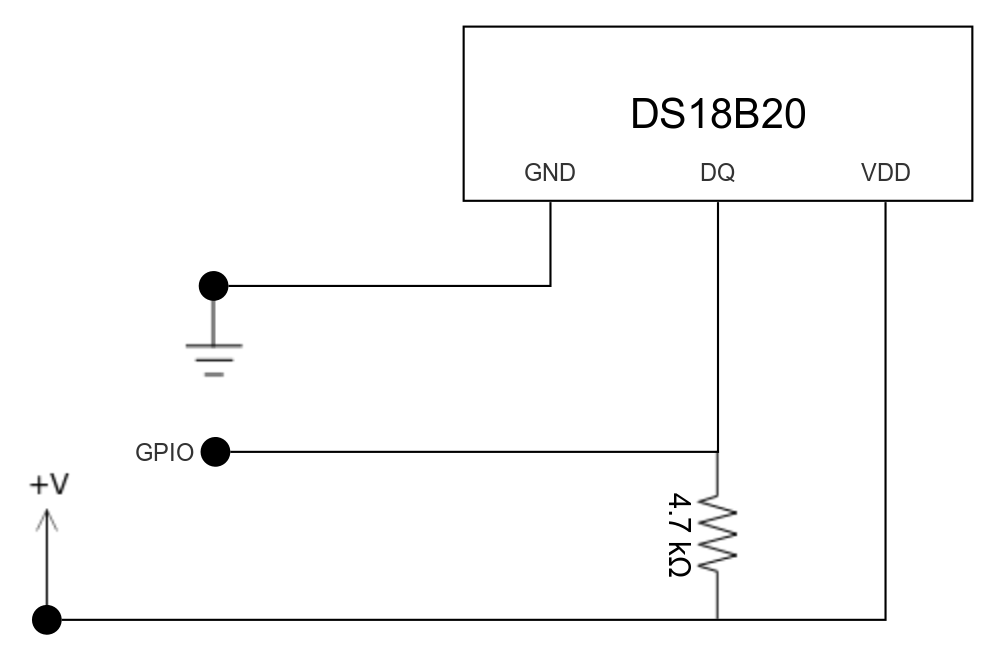
\includegraphics[width=0.6\columnwidth]{HS_14008_temp_circuit.png}
		\label{fig:temperature_sensor_circuit}}
	
	%\qquad
	\subfloat[Sensor within roof box]{
		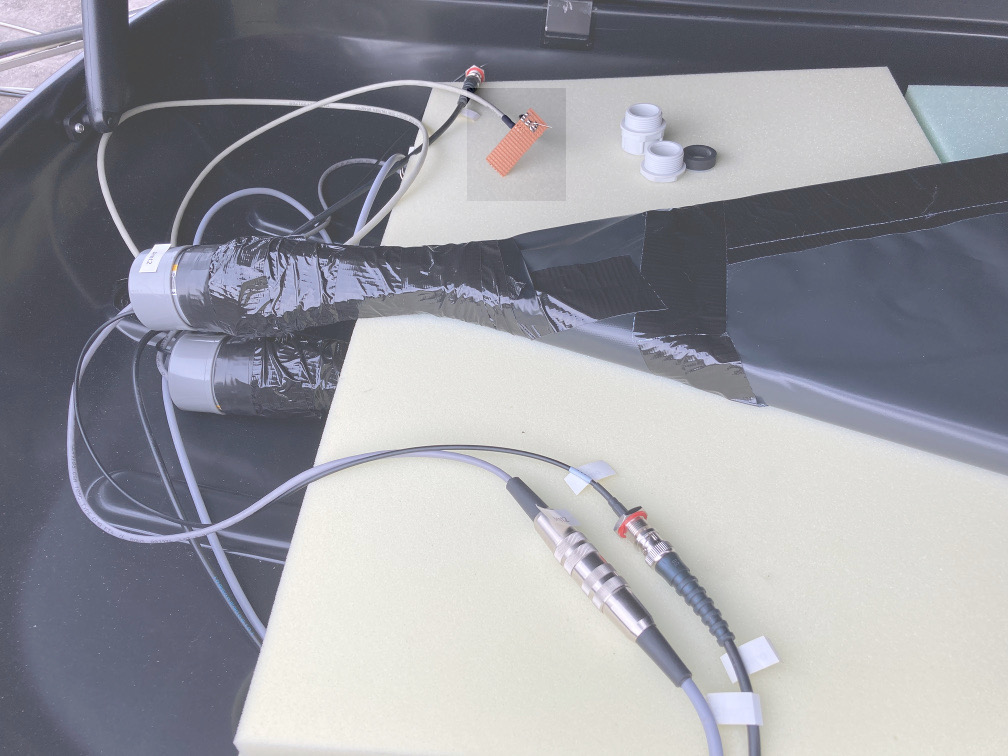
\includegraphics[width=0.55\columnwidth]{temperture_sensor_rescaled.jpg}
		\label{fig:temperature_sensor_in_box}} \\
	
	\caption{(a) Schematic diagram of the DS18B20 temperature sensor circuit, whereby the voltage drain (VDD), ground (GND), and data (DQ) pins connect directly to the voltage supply (+V), ground, and input/output (GPIO) pins of the Raspberry Pi board. (b) Shows the temperature sensor within the roof box, located by the PMTs. The temperature sensor is soldered into the circuit board seen in the top-middle of the image.}
	\vspace{2em}
	\label{fig:temperature_sensor}
\end{figure}


%%%%%%%%%%%%%%%%%%%%%%%%%%%%%%%%%%%%%%%%%%%%%%%%%%%%%%%%%%%%%%%%%%%%%
\subsection{Data Acquisition}
\label{sec:HS14008_data_acqusition}

The new \gls{hisparc} station uses two methods of data acquisition. The singles data and reduced coincidences data (events) are acquired using the typical \gls{hisparc} data acquisition software, but the original coincidences, reduced coincidences, and the temperature data are all acquired by a Raspberry Pi 4. This was done as it allowed us to store the original coincidences data without overloading the \gls{hisparc} servers. A schematic diagram showing the interfaces between the Raspberry Pi and the other hardware is shown in Figure~\ref{fig:14008_RP4}.

\begin{figure}[ht!]
	\center
	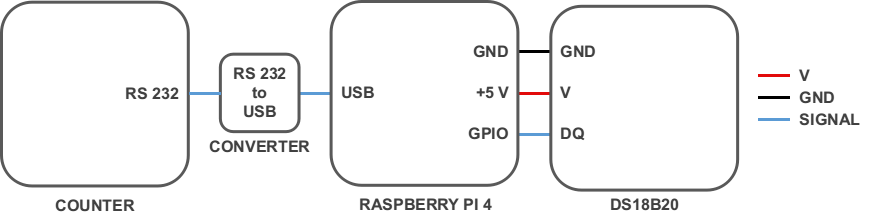
\includegraphics[width=0.8\columnwidth]{14008_data_acq_config.png}
	\caption{Schematic diagram of the HiSPARC station 14008 data acquisition interfaces. Red lines depict a 5~V signal; black lines show ground connection; blue lines depict the 1-wire protocol signal.}
	\label{fig:14008_RP4}
\end{figure}


The Raspberry Pi 4 was used to control the data acquisition by running continuous Python scripts; one for \gls{cr} counts and another for the temperature data. The scripts configured the hardware and output the coincidences and temperature data to local files on the Raspberry Pi. The coincidences and temperature data are both recorded on a 10-second cadence.

The Python scripts were written such that each new day generates a separate file for the coincidences data and temperature data. Within the coincidence files there are no headers and the data begins from line 1. The files contain four columns and the data stored in each column is listed in Table~\ref{tab:HS_14008_coincidences_data}.

\vspace{1em}

\begin{table}[ht!]
	\begin{center}
		\caption{Variables stored in the coincidences files of the HiSPARC 14008 instrument.}
		\label{tab:HS_14008_coincidences_data}
		\begin{tabular}{cp{0.2\linewidth} lp{0.35\linewidth} cp{0.3\linewidth} cp{0.35\linewidth}}
			\hline 
			{\bf Column} & {\bf Item} & {\bf Unit} & {\bf Type} \\ 
			\hline 
			\multirow{2}*{0} & \multirow{2}*{Time Stamp} & YYYY\_MM\_DD & \multirow{2}*{String}  \\ 
			  &  & HH:MM:SS.ffffff & \\ 
			1 & Time*  & Decisecond & Integer, eight digits, zero padded \\ 
			2 & Cumulative Reduced Count* & Counts & Integer, eight digits, zero padded \\ 
			3 & Cumulative Full Count* & Counts & Integer, eight digits, zero padded \\ 
			\hline 
		\end{tabular} 
	\end{center}
	* Since restart
\end{table}

The \gls{nim} counter records the cumulative coincidences count, therefore the reduced and full data stored are also cumulative and thus when reading the data, one must ensure that the difference is calculated between timestamps. In the event of hardware or software failure, or a reboot of the Raspberry Pi, when the Python script re-runs the \gls{nim} counter restarts all values from 0. When reading a file, one must ensure that checks are in place to handle any restarts from zero appropriately, such that no negative counts are calculated from one timestamp to the next during a restart.

Within the temperature files, there are also no headers and the data begins from line 1. The columns in the data files are outlined in Table~\ref{tab:HS_14008_temperature_data}.

\vspace{1em}

\begin{table}[ht!]
	\begin{center}
		\caption{Variables stored in the temperature files of the HiSPARC 14008 instrument.}
		\label{tab:HS_14008_temperature_data}
		\begin{tabular}{c l l l}
			\hline 
			{\bf Column} & {\bf Item} & {\bf Unit} & {\bf Type} \\ 
			\hline 
			\multirow{2}*{0} & \multirow{2}*{Time Stamp} & YYYY\_MM\_DD & \multirow{2}*{String}  \\ 
			  &  & HH:MM:SS.ffffff & \\ 
			1 & Temperature & $^\circ$C & Floating point \\ 
			\hline 
		\end{tabular} 
	\end{center}
\end{table}


The coincidences and temperature data are stored locally, but they are also stored on the University of Birmingham Particle Physics servers as a back-up\footnote{Disk location: /disk/moose/general/epesv001/datadisk/147.188.46.117\_hisparc\_pi/}. Access to the data is not necessarily open-to-all, and to request access, one should contact the System Administrator for the Particle Physics Group Computing Facilities.

The reduced coincidences data are also acquired using the \gls{hisparc} data acquisition software and are stored on the \gls{hisparc} servers. The \gls{hisparc} servers record this data as `events' and the data can be accessed using the methods described in Section~\ref{sec:HS_data}.


%[What is the width of the signals generated by the NIM crate? Is it more or less than the approx. 25ns FWHM of the pulses..? Then relate that to: "The pulse width, Tw, is important only insofar as it determines the maximum rate of pulses that may be represented by the pulse train, since pulses which occur more frequently than 1/Tw cannot be resolved"...]

Data acquisition for station 14008 first began in March 2019. At this early stage of development, data were only acquired using the \gls{hisparc} servers and not the \gls{nim} crate. The use of the \gls{nim} crate started in mid-September 2019, but it was not until mid-January 2020 that the temperature data were first acquired. The availability of data was interrupted during early months of 2020 due to the COVID-19 pandemic affecting our ability to perform crucial work on the station. It is therefore recommended to only use data after August 2020, when both coincidences and temperature data are regularly available.%, are regularly available.



%%%%%%%%%%%%%%%%%%%%%%%%%%%%%%%%%%%%%%%%%%%%%%%%%%%%%%%%%%%%%%%%%%%%%
\subsection{Monitoring Pressure}

As explained in the previous chapter, it was necessary to account for the barometric effect on the muon count rate, for both the singles data and coincidences data. To monitor the pressure, a nearby meteorological station was used, which is part of the \gls{midas} database, and acquired from the \gls{stfc} and \gls{nerc} \gls{ceda} archive.

The \gls{midas} station used is the nearest pressure monitor to the \gls{hisparc} and provides a robust measure of the local atmospheric pressure. The station is located in Coleshill, Warwickshire (ID: 19187), nearby Birmingham International Airport, $\sim 20$~km from the \gls{hisparc} detectors. The pressure is measured at the \gls{midas} station level and a correction for altitude should be small. 

The pressure data are recorded on a 1-hour cadence in units of hPa, with a precision of 0.1~hPa. The time variation of pressure is slow; hence, we linearly interpolated the data to provide a 1-minute sample.


%%%%%%%%%%%%%%%%%%%%%%%%%%%%%%%%%%%%%%%%%%%%%%%%%%%%%%%%%%%%%%%%%%%%%
%%%%%%%%%%%%%%%%%%%%%%%%%%%%%%%%%%%%%%%%%%%%%%%%%%%%%%%%%%%%%%%%%%%%%
\section{Methodology}\label{sec:HS_14008_methods}

\subsection{Atmospheric Corrections}

After considerate review of the methods for temperature correction, the method discussed and used in Chapter~\ref{chap:HiSPARC} was used here, i.e. using a linear relationship between \glspl{cr} and temperature:

\begin{equation}
\mathrm{ln} \left( \frac{N}{N_0} \right) = - \alpha \, \Delta T \, ,
\label{eq:tempcorr_14008}
\end{equation}
%
where $N$ is a single measurement; $N_0$ may be considered as the mean count rate over the given time-period of observations; $\Delta T = T - T_0$ is the deviation in temperature from the average ($T_0$) in the given time-period; and $\alpha$ is the temperature coefficient. However, the method was tweaked slightly. The steps for correcting for the effect of temperature were:

\begin{itemize}
	\item{To remove any long-term temperature trends over a month of data, the \gls{cr} and temperature data were smoothed using a 24-hr moving mean. Using the linear relationship between the smoothed \glspl{cr} and temperature (defined by equation~(\ref{eq:tempcorr_14008}), where the $N$ and $T$ are the smoothed data), the long-term temperature relationship was fitted and corrected in the data.}

	\item{After correcting for the long-term temperature relationship, for each day the temperature correction was applied again to remove the daily variations (i.e. using equation~(\ref{eq:tempcorr_14008}), where the $N$ denotes the de-trended \gls{cr} data and $T$ denotes the raw temperature data; the de-trended \gls{cr} and raw temperature data were smoothed again using a 24-hr moving mean for $N_0$ and $T_0$). The temperature relationship was fitted and corrected in the data, day-by-day.}
\end{itemize}


The above procedure was adopted because during the initial temperature corrections, it was found that without removing the long-term temperature relationship there was still some long-term covariance between the temperature and the \gls{cr} count. In addition, we found that the previous correction procedure induced jumps in the data between days; this method of using smoothed data for the values of $N_0$ and $T_0$ ensured that there was a smooth transition in the corrected data between days.

Using the theory outlined in Section~\ref{sec:HS_P_corr} we were able to perform the barometric correction of the singles data and coincidences data, whereby a linear fit was made using the model defined by equation~(\ref{eq:presscorr3}). Similarly, the barometric correction was performed over durations of 1-month at a time.

For reasons discussed in Section~\ref{sec:HS_14008_atmospheric_correction} the temperature correction was, in practice, only applied to the singles data. When correcting the atmospheric effects on the singles data, the temperature correction was performed first and was followed by the pressure correction.



\subsection{Observation Statistics}\label{sec:HS_14008_method_obs}

The probability distribution of the number of \gls{cr} counts in a fixed interval of time follows the Poisson distribution, defined by:
%
\begin{equation}
P(k; \, \lambda) = \frac{\lambda^k \, e^{-\lambda}}{k!} \, ,
\label{eq:poisson_PDF}
\end{equation}
%
where $k$ is the number of events, which is always an integer, and $\lambda$ is the mean value of the number of events per interval, i.e. the expected number \citep{lista_statistical_2016}. Under the Poisson distribution, the mean and the variance are both equal to $\lambda$. For a large value of $\lambda$, the Poisson distribution can be approximated by a Gaussian distribution having mean, $\lambda$, and standard deviation, $\sqrt{\lambda}$ \citep{lista_statistical_2016}.

The Poisson distribution is also additive such that if two variables, $n_1$ and $n_2$, follow Poisson distributions, with mean values $\lambda_1$ and $\lambda_2$, respectively, then the sum also follows a Poisson distribution:
%
\begin{equation}
P(n; \, \lambda_1, \lambda_2) = P(n; \, \lambda_1 + \lambda_2) \, ,
%\sum_{min}^{max} P(k; \, \lambda) P(k; \, \lambda) =
%p. 40 in Lista, L. (2016) 
\label{eq:poisson_additive_PDF}
\end{equation}
%
where $n = n_1 + n_2$ \citep{lista_statistical_2016}.

Using this information, it was possible to use a Monte Carlo sampling algorithm to determine the mean level and noise of the \gls{hisparc} 14008 station's data. We sampled the posterior using the \textsc{PyMC3} No-U-Turn Sampler (NUTS) extension to a Hamiltonian Monte Carlo (HMC) sampling algorithm \citep{salvatier_probabilistic_2016} with a Poisson distribution likelihood function. For the mean count rate we used a prior of $\mathcal{U}(3000,6000)$~counts/min and for the noise rate we used a prior of $\mathcal{U}(0.0,5.0)$~counts/min. In both instances, after a burn in of 2000 iterations, we used 5000 iterations on 4 chains to explore the posterior parameter space. Convergence was interrogated using the Gelman-Rubin $\widehat{R}$ diagnostic factor \citep{gelman_inference_1992}, using the criteria that chains did not converge if $\widehat{R} > 1.01$.

In addition, with this knowledge artificial data were created, to simulate the detector's response to space weather events as a further study of the capabilities of the new station configuration. The artificial data were generated using the method discussed in Appendix~\ref{app:GLE_sims}, to simulate the mean count rate and noise properties of the station. It was possible to inject \glspl{gle} into the artificial data with differing properties, to determine the likelihood of observing such events.

During the analysis of simulated data, we used a series of statistical tests to determine whether we could observe the injected \glspl{gle}. We used the fact that count data obey a Poisson distribution to compute the probability of statistically significant spikes in the data. The Poisson cumulative distribution function is given by:
%
\begin{equation}
F(k; \, \lambda) = \sum_{i=0}^{k}  \frac{\lambda^i \, e^{-\lambda}}{i!} \, .
\label{eq:poisson_CDF}
\end{equation}


Using this expression, the probability that a time interval observes $k$ or more events, by chance, given the mean level, $\lambda$, is therefore given by: 
%
\begin{equation}
p(k) = 1 \, - \, F(k-1; \, \lambda) \, .
\label{eq:poisson_SF}
\end{equation}

If $k\gg\lambda$ then $p(k)\to0$. The probability that we fail to observe a cadence with $k$ or more events is: $1 \, - \, p(k)$; thus the probability of failing to observe any time interval with $k$ or more events in $N$-cadences is $[1 \, - \, p(k)]^N$. Therefore, the probability to find at least one event at or above $k$ in N-cadences, by chance, is:
%
\begin{equation}
p_N = 1\, - \, [1 \, - \, p(k)]^N \, ,
\label{eq:poisson_p_N}
\end{equation}
%
where a low value for $p_N$ indicates that the observed event is very unlikely to be a statistical fluctuation, and therefore a potential detection.

This can be generalised using the cumulative binomial distribution \citep{basu_asteroseismic_2017}. The probability of finding at least $r$ occurrences in $N$-cadences, by chance, at or above $k$, given the mean level, $\lambda$, is given by equation~(\ref{eq:poisson_binom_CDF}), which is equal to equation~(\ref{eq:poisson_p_N}) when $r=1$,
%
\begin{equation}
p[r; p(k), N] = \sum_{r=r}^{N} \binom{N}{r} \, p(k)^r \, [1 \, - \, p(k)]^{N-r} \, .
\label{eq:poisson_binom_CDF}
\end{equation}

By applying equation~(\ref{eq:poisson_binom_CDF}) to the data, we were able to test whether there were any significant events against a certain probability threshold. Again, a low value for $p[r; p(\lambda), N]$ indicates that the event is very unlikely to happen by chance alone, and therefore a potential detection. The chosen probability threshold during all tests was 10\%, i.e., this corresponds to a 10\% chance of observing an excessive measurement as a statistical fluctuation.

The choice of $N$ in this binomial test varies the required measurement threshold \citep{basu_asteroseismic_2017}. In the tests performed we chose a value of $N=720$ (i.e. $\sim2$~hours for measurements with a 10-second cadence). This value of $N$ was chosen as it is approximately the average \gls{fwhm} for \glspl{gle} \citep{strauss_pulse_2017}. In a 48-hour window, observing with a cadence of 10-seconds, we have $n=17280$ total points; however, using $N=720$ gives $n/N\approx24$ independent time-windows to test. On average, we would therefore expect to measure approximately $0.1 \times 24 \simeq 2.4$ points exceeding the threshold due to statistical fluctuations. These represent unwanted, false-positive detections, but allow us to judge whether there is any potential significance in a given data set, depending on how the number of excessive measurements compares to this level. Furthermore, a space weather event, such as a \gls{gle} will produce excess events clustered in time; whilst false-alarm events will be randomly distributed.


Another frequentist test that was used makes use of the assumption that the Poisson distribution tends towards a Gaussian distribution when the mean value is sufficiently large. An excess in counts, compared to the mean value, can be quantified as:
%s = x - mu
%z = s / std
%
\begin{equation}
s = k - \lambda \, ,
\label{eq:poisson_excess}
\end{equation}
%
where $s$ is the excess in the signal, $k$ is the measured signal and $\lambda$ is the expected value, or background signal \citep{lista_statistical_2016}. The significance can then be approximated by:
%
\begin{equation}
Z = \frac{s}{\sigma} \, ,
\label{eq:poisson_significance}
\end{equation}
%
where $\sigma$ is the expected standard deviation, which for a Poisson distribution is $\sqrt{\lambda}$. In this work we used both $Z = 3$ and $Z = 5$ significance levels to determine the existence of excess signals.

%As a further test we also analysed re-sampled versions of the artificial data. This allowed us to reduce the Poisson noise, with the ambition of reducing the noise such to allow us to observe lower amplitude space weather events. 
We also ran the statistics tests on 1-minute and 5-minutes averages of the artificial data. The statistics tests were run with the same underlying principles; however, instead of using the Poisson cumulative distribution in equation~(\ref{eq:poisson_SF}), we instead used the Gaussian cumulative distribution for the averaged data with mean, $\mu = \lambda$, and standard deviation, $\sigma = \sqrt{\lambda/n}$, where $n$ represents the number of data points used in the average. %Similarly, using the Gaussian distribution with mean, $\mu = \lambda$, and  standard deviation, $\sigma = \sqrt{\lambda/n}$, in equation~(\ref{eq:poisson_significance}).



%%%%%%%%%%%%%%%%%%%%%%%%%%%%%%%%%%%%%%%%%%%%%%%%%%%%%%%%%%%%%%%%%%%%%
%%%%%%%%%%%%%%%%%%%%%%%%%%%%%%%%%%%%%%%%%%%%%%%%%%%%%%%%%%%%%%%%%%%%%
\section{Atmospheric Corrections}\label{sec:HS_14008_atmospheric_correction}

%%%%%%%%%%%%%%%%%%%%%%%%%%%%%%%%%%%%%%%%%%%%%%%%%%%%%%%%%%%%%%%%%%%%%

\subsection{Temperature Correction}\label{sec:HS_14008_T_corr}

Using the method outlined in Section~\ref{sec:HS_14008_methods} we applied the temperature correction. The temperature correction was first applied between the coincidences data and the temperature measured inside the roof box. The typical relationship between the data and the temperature is shown for a single day in Figure~\ref{fig:14008_coincidences_v_T_corr}.

\begin{figure}[ht!]
	\centering
	\subfloat[Coincidences versus temperature]{
		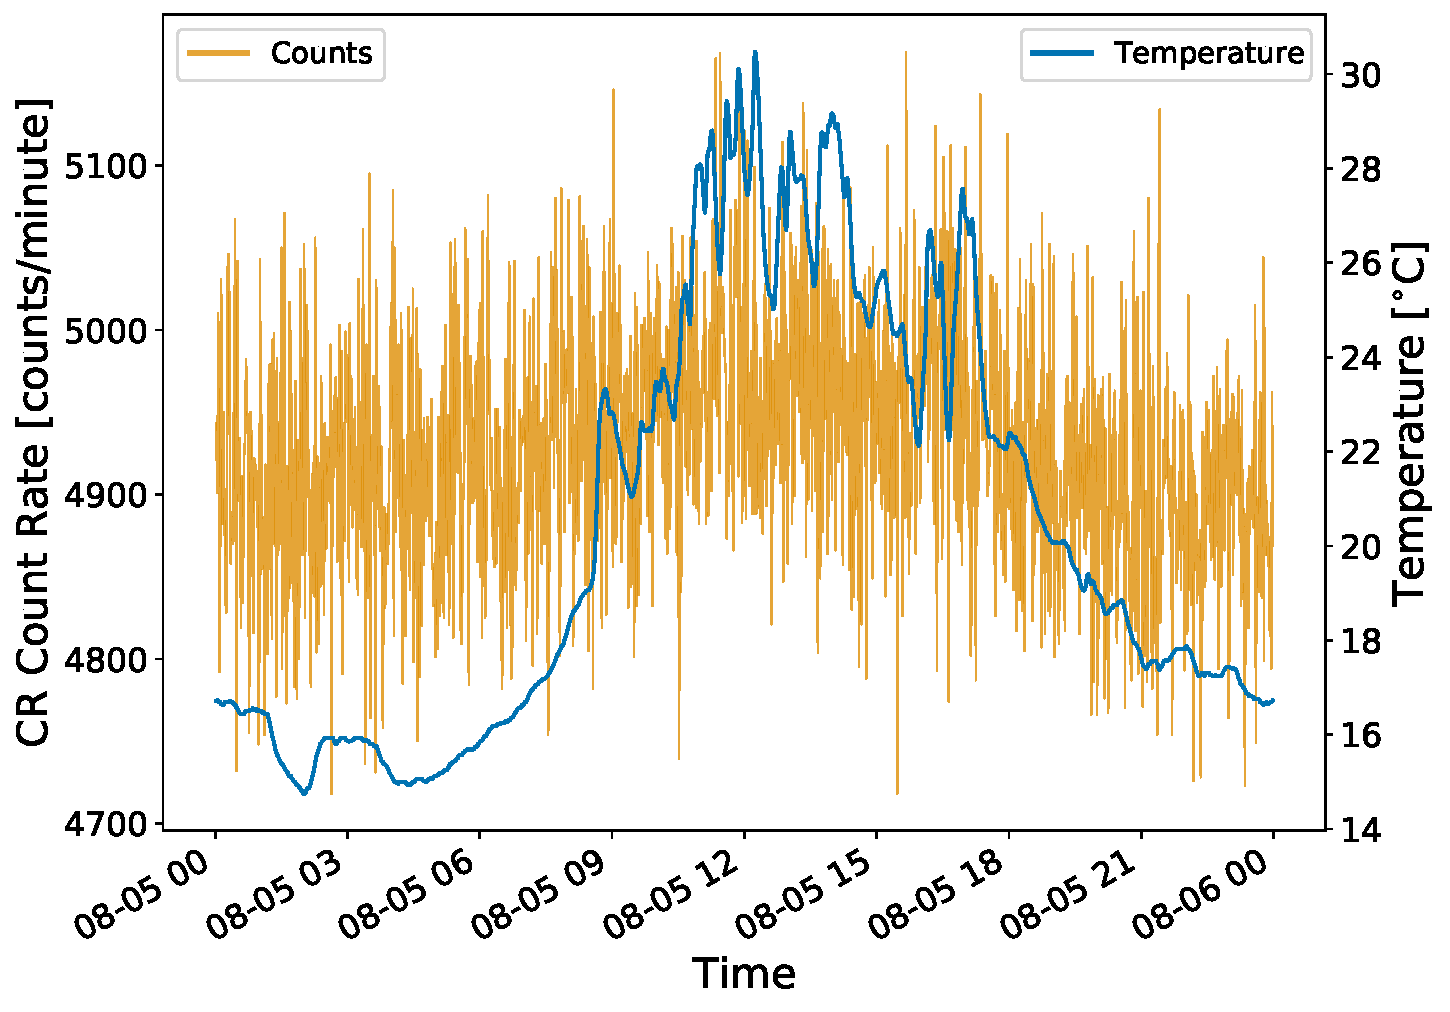
\includegraphics[width=0.48\columnwidth]{coincidences_v_T.pdf}
		\label{fig:HS_14008_coincidences_v_T}}
	%\qquad
	\subfloat[Correlation of coincidences and temperature]{
		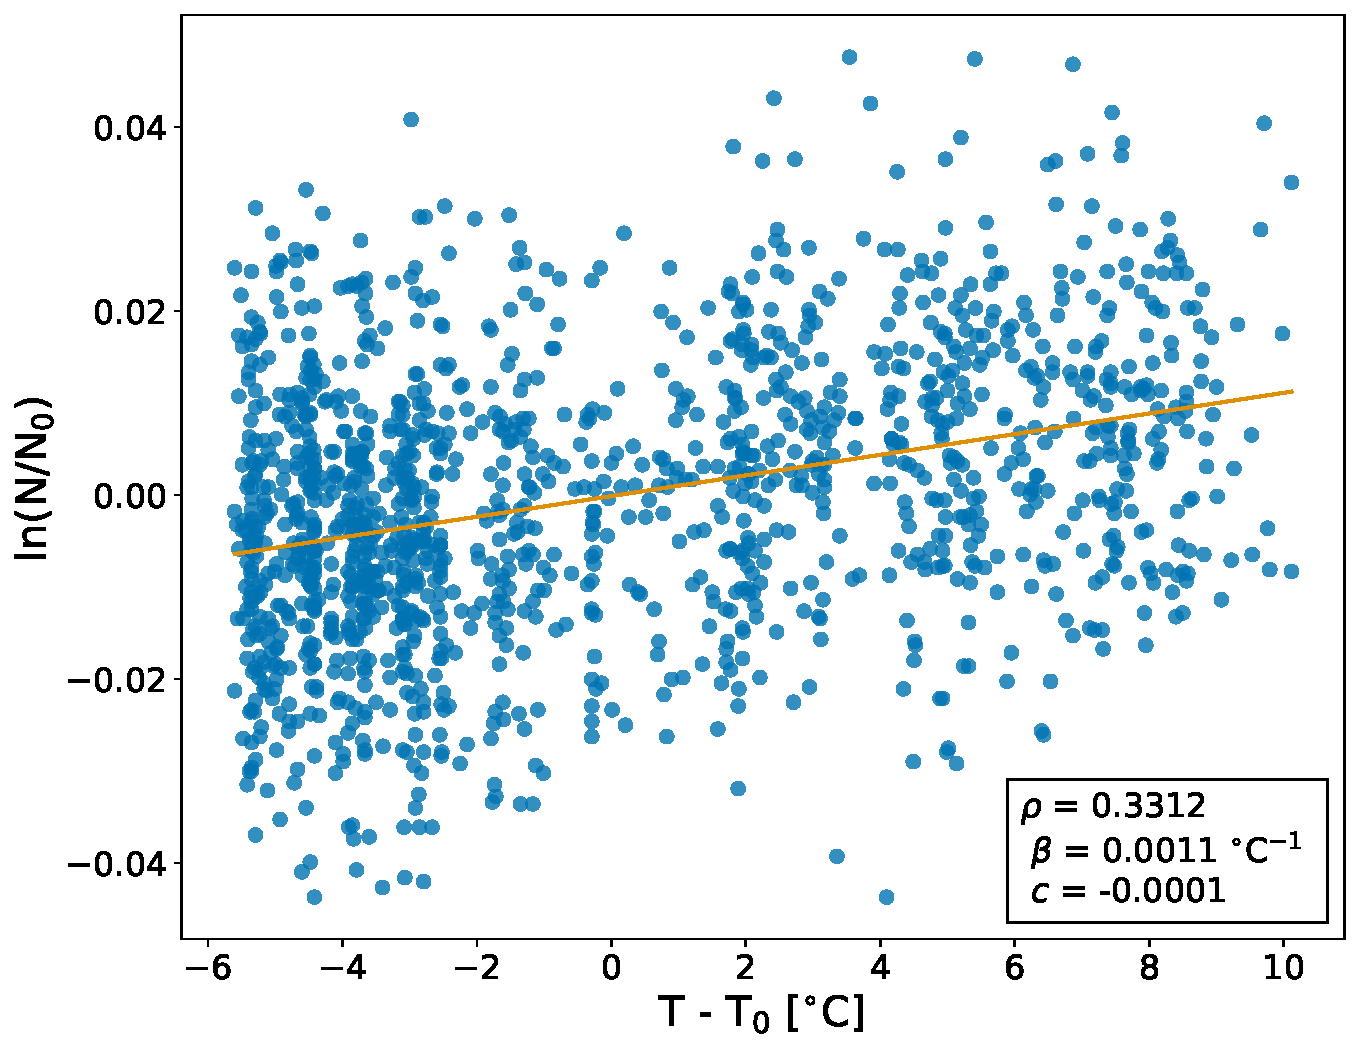
\includegraphics[width=0.48\columnwidth]{fit_coincidences_v_T.pdf}
		\label{fig:HS_14008_coincidences_alpha}} \\
	
	\caption{The relationship between the original coincidences data and the temperature within the roof box over a single day. (a) Shows the comparison between coincidences data (orange) and temperature data (blue), where the units of time on the x-axis are, MM-DD HH; (b) shows the correlation between the coincidences counts and temperature, and the fitted line to calculate the correction coefficient.}
	\label{fig:14008_coincidences_v_T_corr}
\end{figure}

We see from Figure~\ref{fig:14008_coincidences_v_T_corr} that there is a weak correlation between the temperature within the roof box and the \gls{cr} counts. Noting the common adage: ``correlation does not necessarily imply causation", we do not expect that the relationship between the coincidences and the temperature is causal. For this relationship to be causal, we require the increase in temperature of the \glspl{pmt} to cause an increase in count rate in the coincidences. We show later in Section~\ref{sec:HS_14008_observations} that the \gls{pmt} thermal noise, which has a strong diurnal component, does not bleed through into the noise on the coincidences data. The weak correlation is a consequence of the rotation of the Earth meaning detectors look in
different directions over the course of a day with a rise in temperature and \gls{cr} counts at local noon \citep{parker_theory_1964, mishra_study_2007, mishra_cosmic_2008}. There is an increase in temperature around local noon as the Sun is overhead of the station, and the variation in the \gls{cr} anisotropy in the interplanetary space causes a diurnal variation which is maximal when the detector is aligned with the Sun. We concluded that it was therefore not necessary to correct the coincidences data for the effects of temperature.


It was necessary to correct the singles data for the effects of temperature; this was one of the main reasons for introducing the measure of temperature within the roof box. One can see the relationship between the singles rates and the temperature in Figure~\ref{fig:HS_14008_temperature_vs_CR}.

\begin{figure}[ht!]
	\centering
	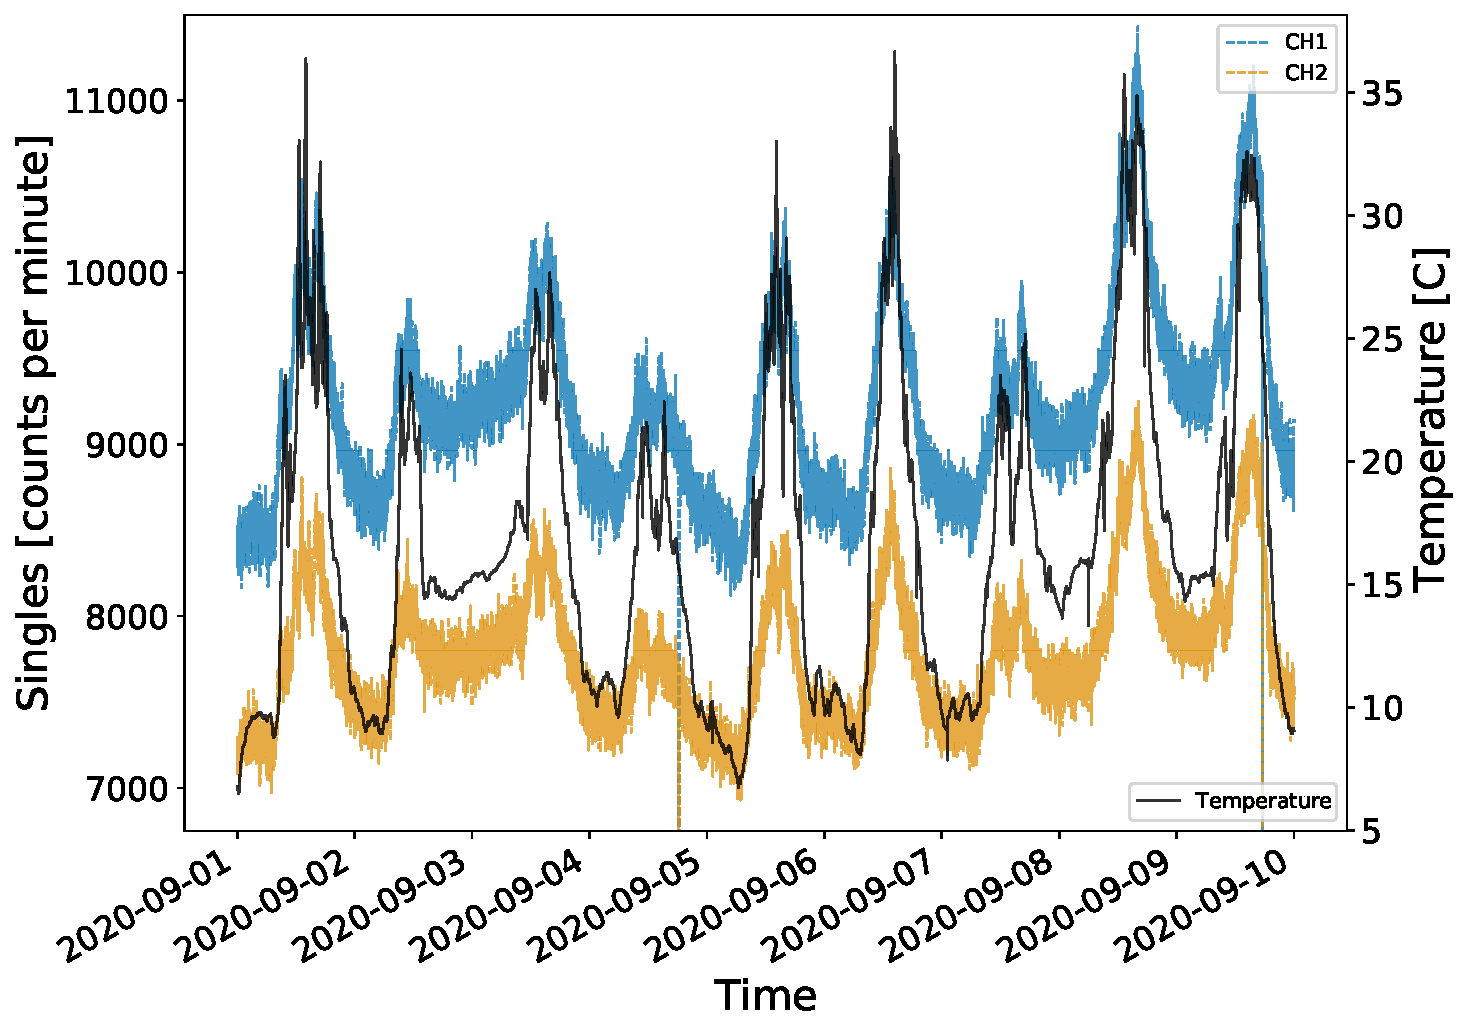
\includegraphics[width=0.7\columnwidth]{HS_14008_CR_v_T_sept2020.pdf}
	\caption{The relationship between the singles data (blue and orange lines) and the temperature within the roof box (black line). The units of time on the x-axis are, YYYY-MM-DD.}
	\label{fig:HS_14008_temperature_vs_CR}
\end{figure}


Figure~\ref{fig:HS_14008_temperature_vs_CR} shows a strong relationship between the temperature inside the roof box (i.e. effectively the temperature of the \glspl{pmt}) and the singles count rates. As expected, the \glspl{pmt} were sensitive to thermal variations, which induced thermal noise, and here we can see this is well-demonstrated. We showed in Chapter~\ref{chap:HiSPARC} that the atmospheric temperature was useful for correcting for the temperature variations in the singles rates, but not completely effective. The reason was because the temperature within the roof box is not the same as the atmospheric temperature. The typical relationship between the singles data and temperature of the \gls{pmt} is shown for a single day in Figure~\ref{fig:14008_CR_V_T_corr}.

\begin{figure}[ht!]
	\centering
	\subfloat[Comparison of singles and temperature]{
		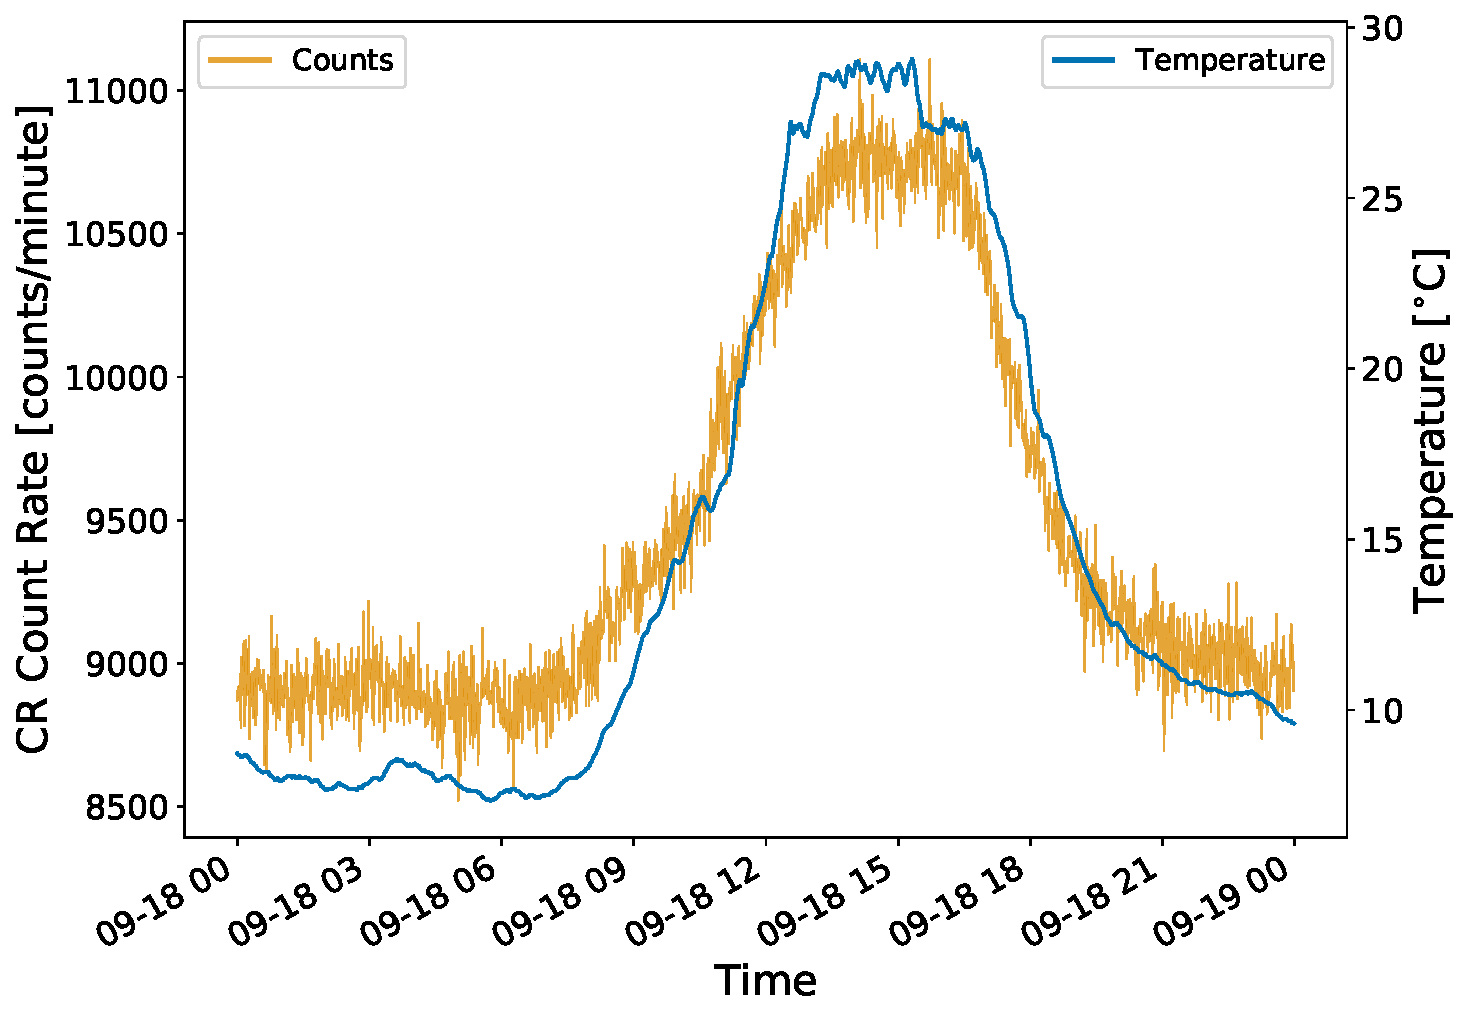
\includegraphics[width=0.48\columnwidth]{CR_v_T.pdf}
		\label{fig:HS_14008_CRvT}}
	%\qquad
	\subfloat[Correlation of singles and temperature]{
		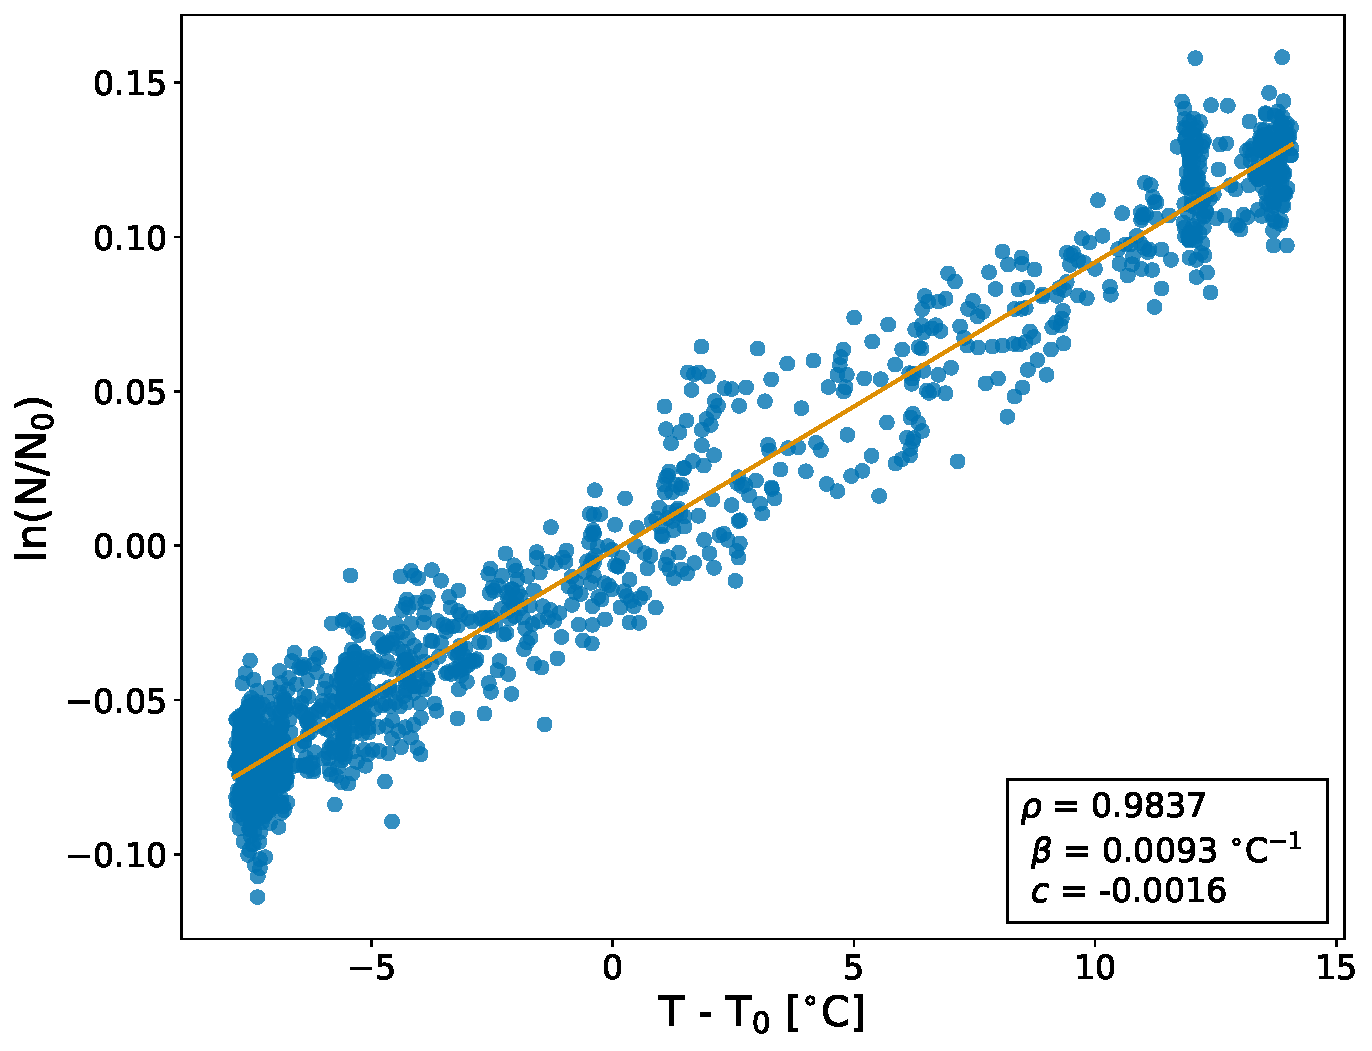
\includegraphics[width=0.48\columnwidth]{fit_CR_v_T.pdf}
		\label{fig:HS_14008_alpha}} \\
	
	\caption{The relationship between the singles data and the temperature within the roof box over a single day. (a) Shows the comparison between singles data (orange) and temperature data (blue), where the units of time on the x-axis are: MM-DD HH; (b) shows the correlation between the singles counts and temperature, and the fitted line to calculate the correction coefficient.}
	\label{fig:14008_CR_V_T_corr}
\end{figure}

The relationship between the singles data and the temperature inside the roof box is much stronger than the relationship between the atmospheric temperature and singles data, which was shown in Chapter~\ref{chap:HiSPARC}. The temperature correction was applied using the linear fit between the singles data and the temperature inside the roof box. For comparison, and to show the success of this method at removing the temperature variation in the singles data, an example of the raw and corrected singles data are shown in together in Figure~\ref{fig:HS_14008_corrected_singles}. 

\begin{figure}[ht!]
	\centering
	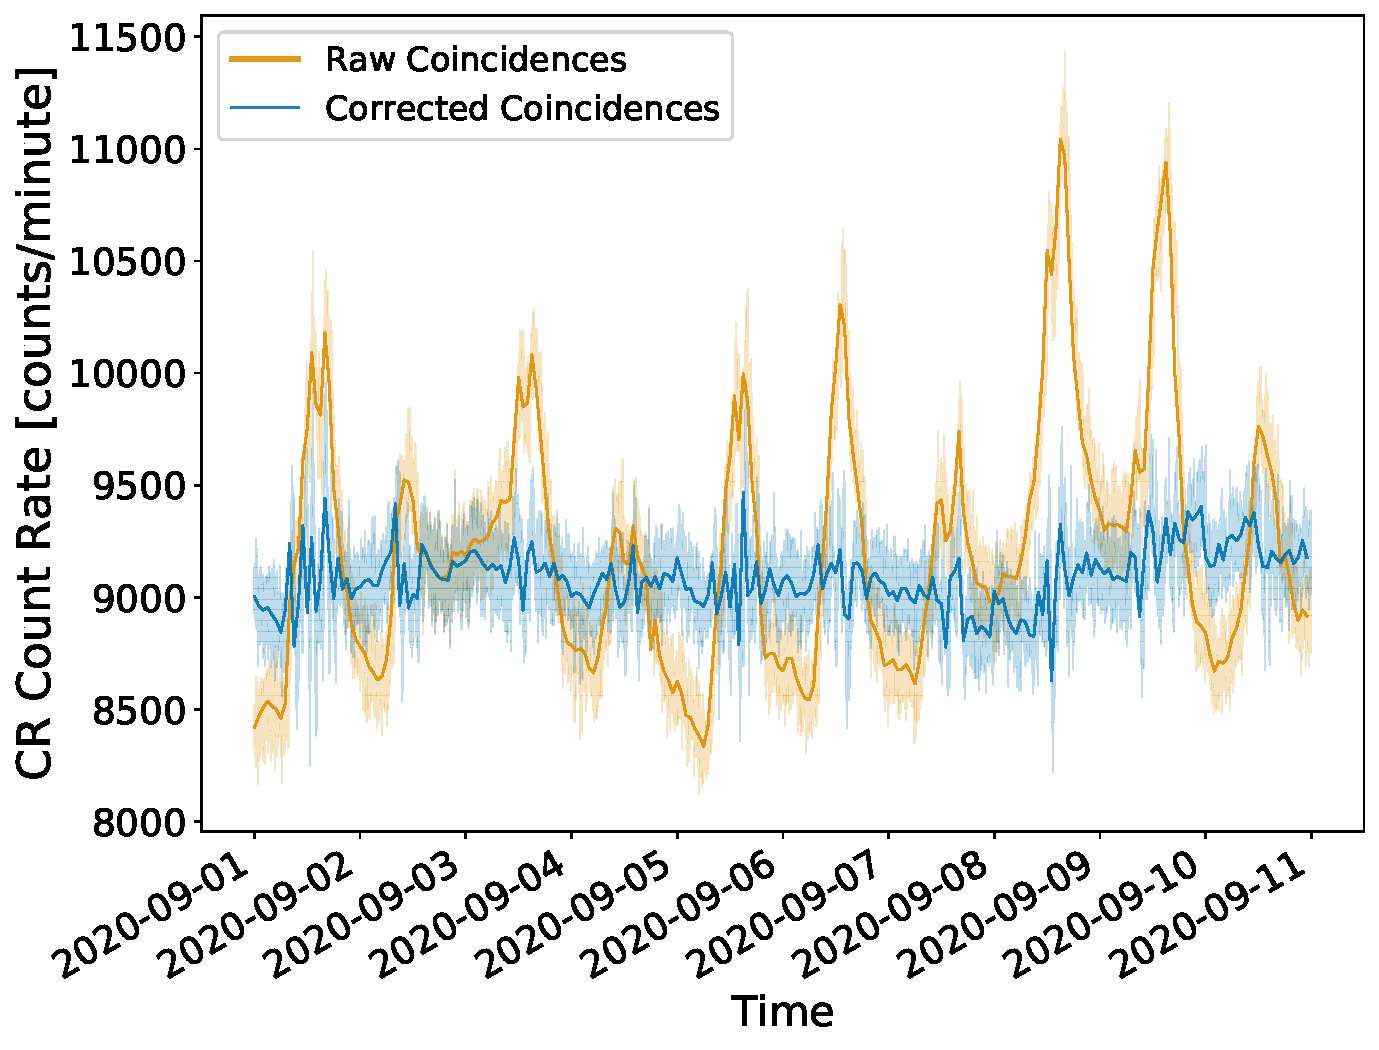
\includegraphics[width=0.6\columnwidth]{raw_vs_corrected_singles.pdf}
	\caption{The singles data before (orange line) and after (blue line) the temperature correction process. The hourly resampled data are over-plotted to highlight the main variation in the data. The units of time on the x-axis are, YYYY-MM-DD.}
	\label{fig:HS_14008_corrected_singles}
\end{figure}

In Figure~\ref{fig:HS_14008_corrected_singles} we see that the large, diurnal excursions are adequately removed from the singles data after this correction. This method of temperature correction was routinely applied to the singles data. %However, the corrected data were not stored on the \gls{hisparc} servers.


An additional benefit of the temperature monitor in the box of station 14008 was that it was also suitable for providing an estimate of the temperature inside the roof-boxes of the detectors that make up \gls{hisparc} station 14001; hence the temperatures of those \glspl{pmt}. Both station 14001 and station 14008 are located on the roof of Poynting physics building at University of Birmingham, therefore they are exposed to the same meteorological conditions and it is likely that the temperature inside one box is similar to the temperature inside each box. Figure~\ref{fig:HS_14008_14001_vs_T} shows a comparison between the singles of the two stations, and the temperature within the box of station 14008.


\begin{figure}[ht!]
	\centering
	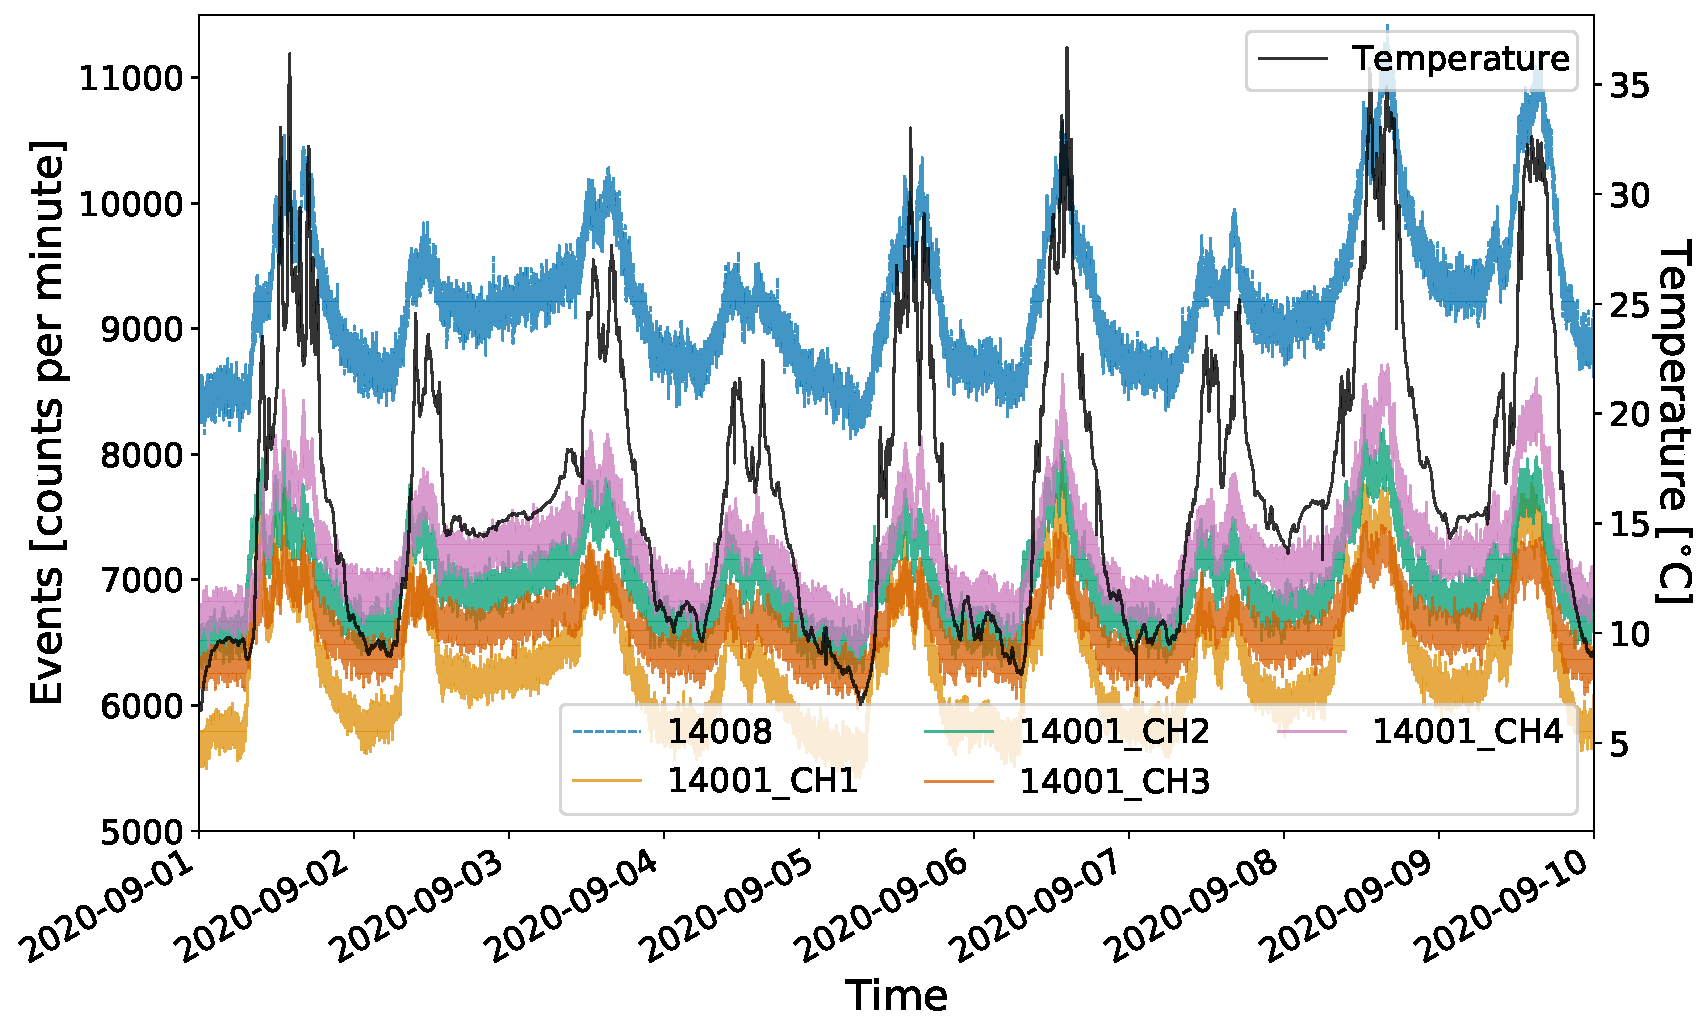
\includegraphics[width=0.9\columnwidth]{HS_14008_vs_14001_and_temp.pdf}
	\caption{Comparison between HiSPARC station 14001 singles data and the singles data and temperature measured by station 14008. Black line: the temperature within the roof box of station 14008; dashed, blue line: HiSPARC station 14008 singles data; solid, orange, green, red, and purple lines: HiSPARC station 14001 singles data. The units of time on the x-axis are, YYYY-MM-DD.}
	\label{fig:HS_14008_14001_vs_T}
\end{figure}

In Figure~\ref{fig:HS_14008_14001_vs_T} we see a good agreement between the singles acquired by both stations. Therefore, it is possible to also use this temperature data to correct for the effects of thermal fluctuations in the singles rates of \gls{hisparc} station 14001.



%%%%%%%%%%%%%%%%%%%%%%%%%%%%%%%%%%%%%%%%%%%%%%%%%%%%%%%%%%%%%%%%%%%%%
%%%%%%%%%%%%%%%%%%%%%%%%%%%%%%%%%%%%%%%%%%%%%%%%%%%%%%%%%%%%%%%%%%%%%
\subsection{Barometric Correction}\label{sec:HS_14008_P_corr}


Using the method outlined in Section~\ref{sec:HS_14008_methods} we were able to perform the barometric correction between the interpolated pressure data and coincidences and singles data. Figure~\ref{fig:14008_CR_V_P_corr} shows a comparison plot of the smoothed coincidences and atmospheric pressure data sets.


\begin{figure}[ht!]
	\centering
	\subfloat[Comparison between coincidences and pressure]{
		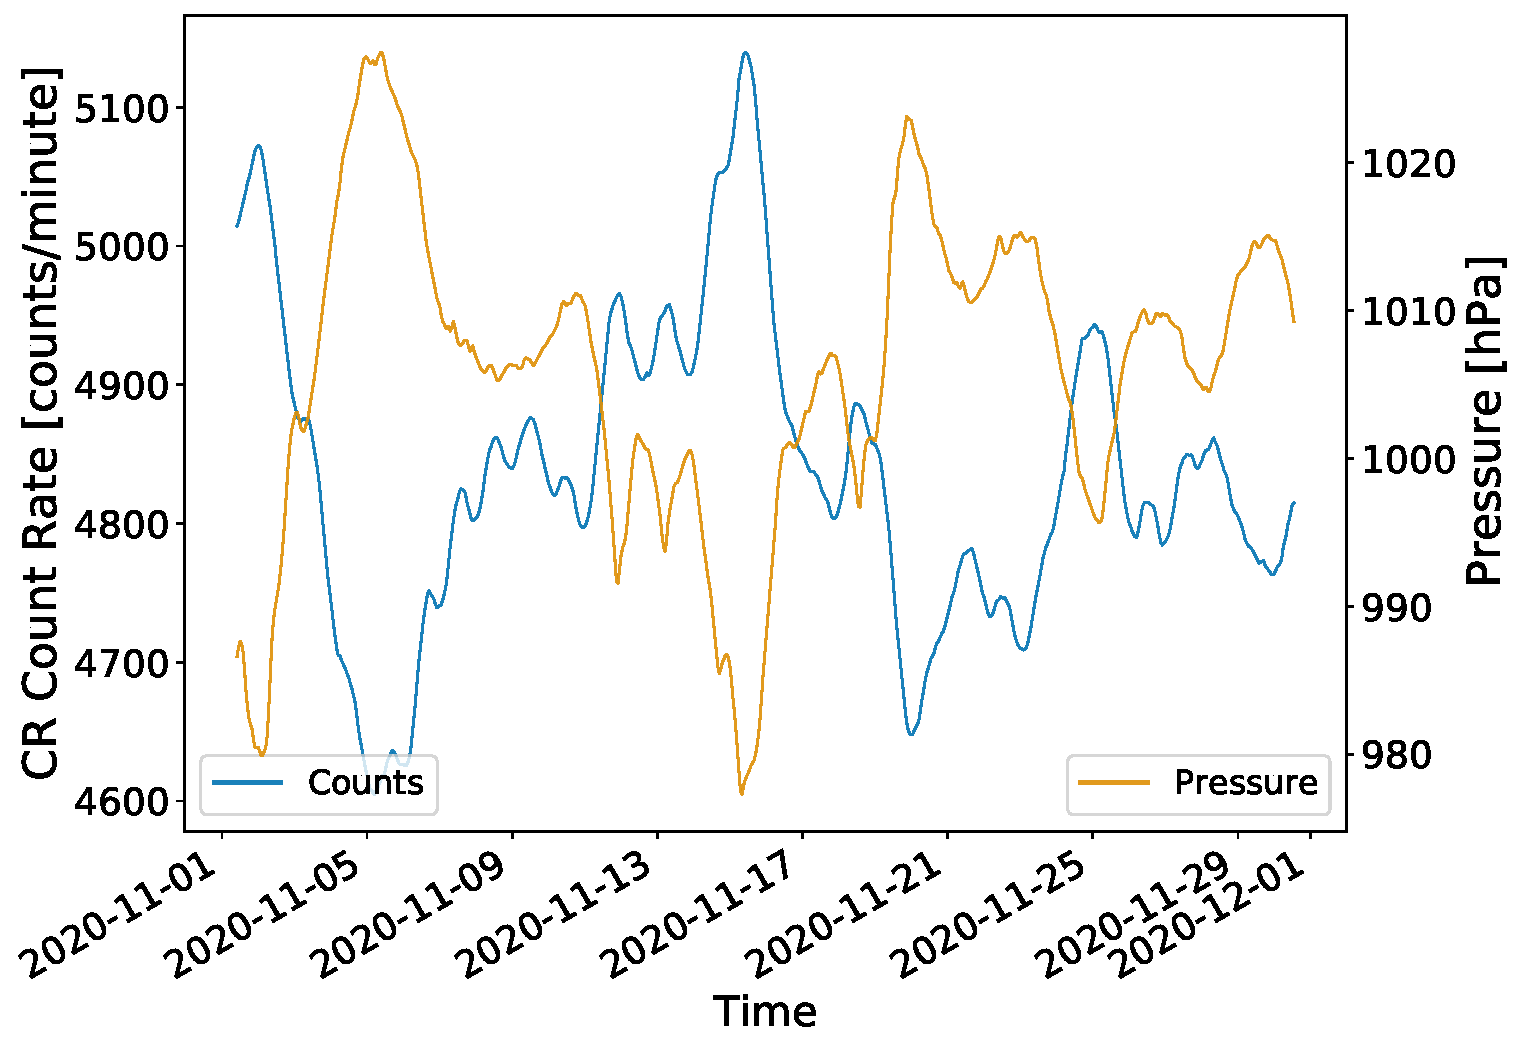
\includegraphics[width=0.48\columnwidth]{CR_v_P.pdf}
		\label{fig:HS_14008_CRvP}}
	%\qquad
	\subfloat[Correlation between coincidences and pressure]{
		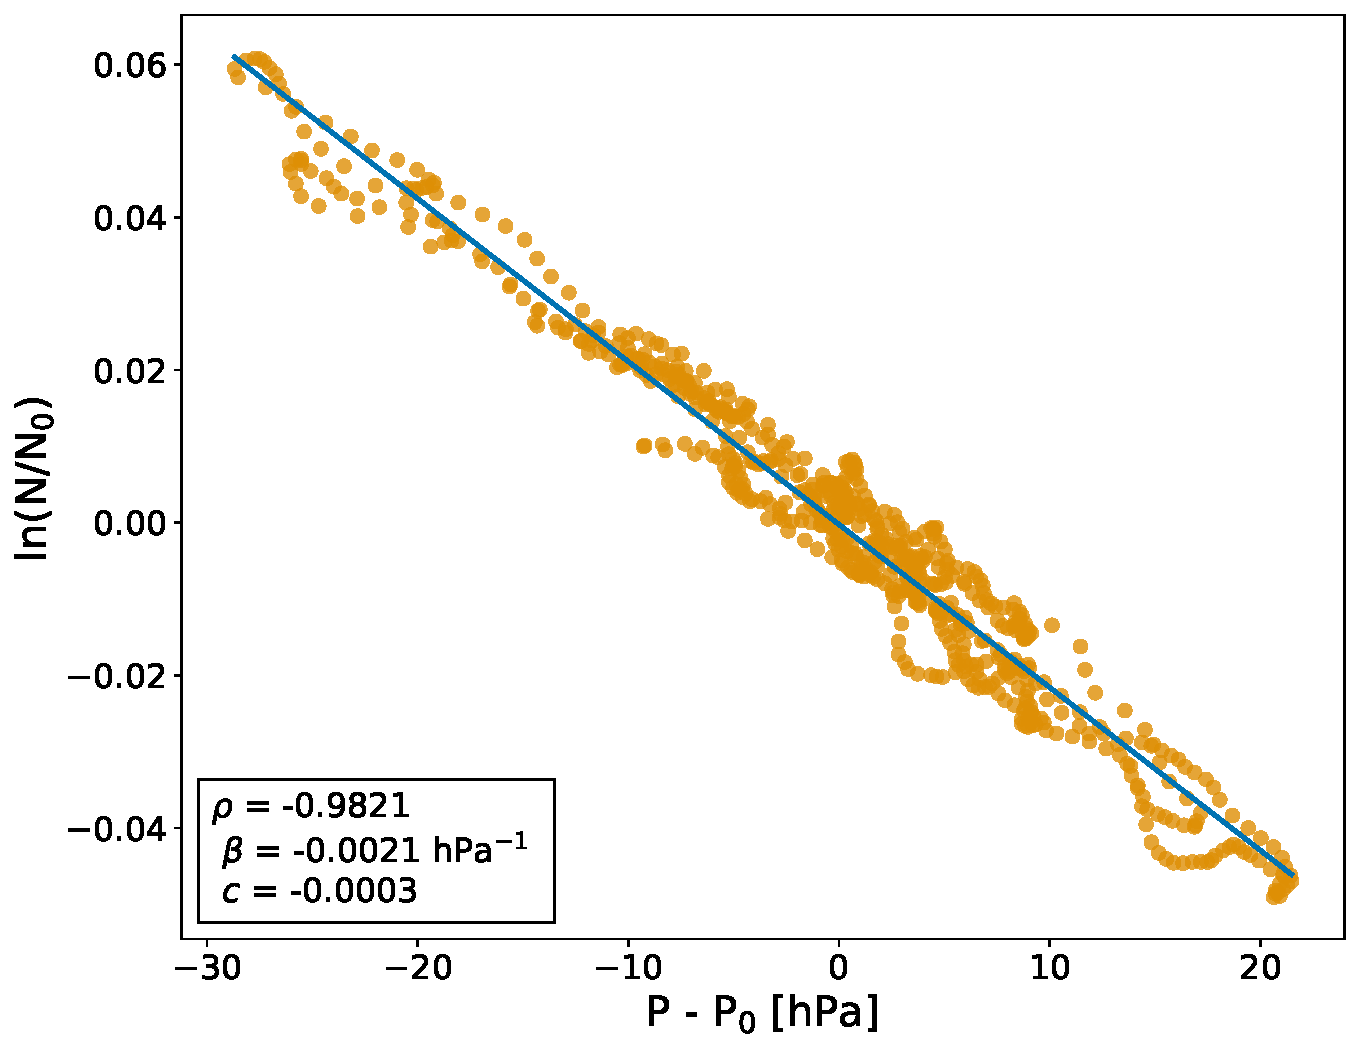
\includegraphics[width=0.48\columnwidth]{fit_CR_v_P.pdf}
		\label{fig:HS_14008_beta}} \\
	
	\caption{The relationship between the smoothed, original coincidences data and the atmospheric pressure. (a) Shows the comparison between coincidences data (orange) and pressure data (blue), both with a 12-hour box-bar smoothing applied, to highlight the relationship and the units of time on the x-axis are: YYYY-MM-DD; (b) shows the correlation between the coincidences counts and pressure and the fitted line to calculate the correction coefficient.}
	\label{fig:14008_CR_V_P_corr}
\end{figure}



As expected, Figure~\ref{fig:14008_CR_V_P_corr} shows the strong negative correlation between \gls{cr} counts and atmospheric pressure. We were able to fit the linear model to the observed data, and the negative barometric coefficient was used to correct the data. For comparison, and to show the success of this method at removing the pressure variation, the raw and corrected coincidences data are shown in Figure~\ref{fig:HS_14008_corrected_coincidences}. It is clear from Figure~\ref{fig:HS_14008_corrected_coincidences} that the large excursions are adequately removed from the data after the correction.


\begin{figure}[htbp!]
	\centering
	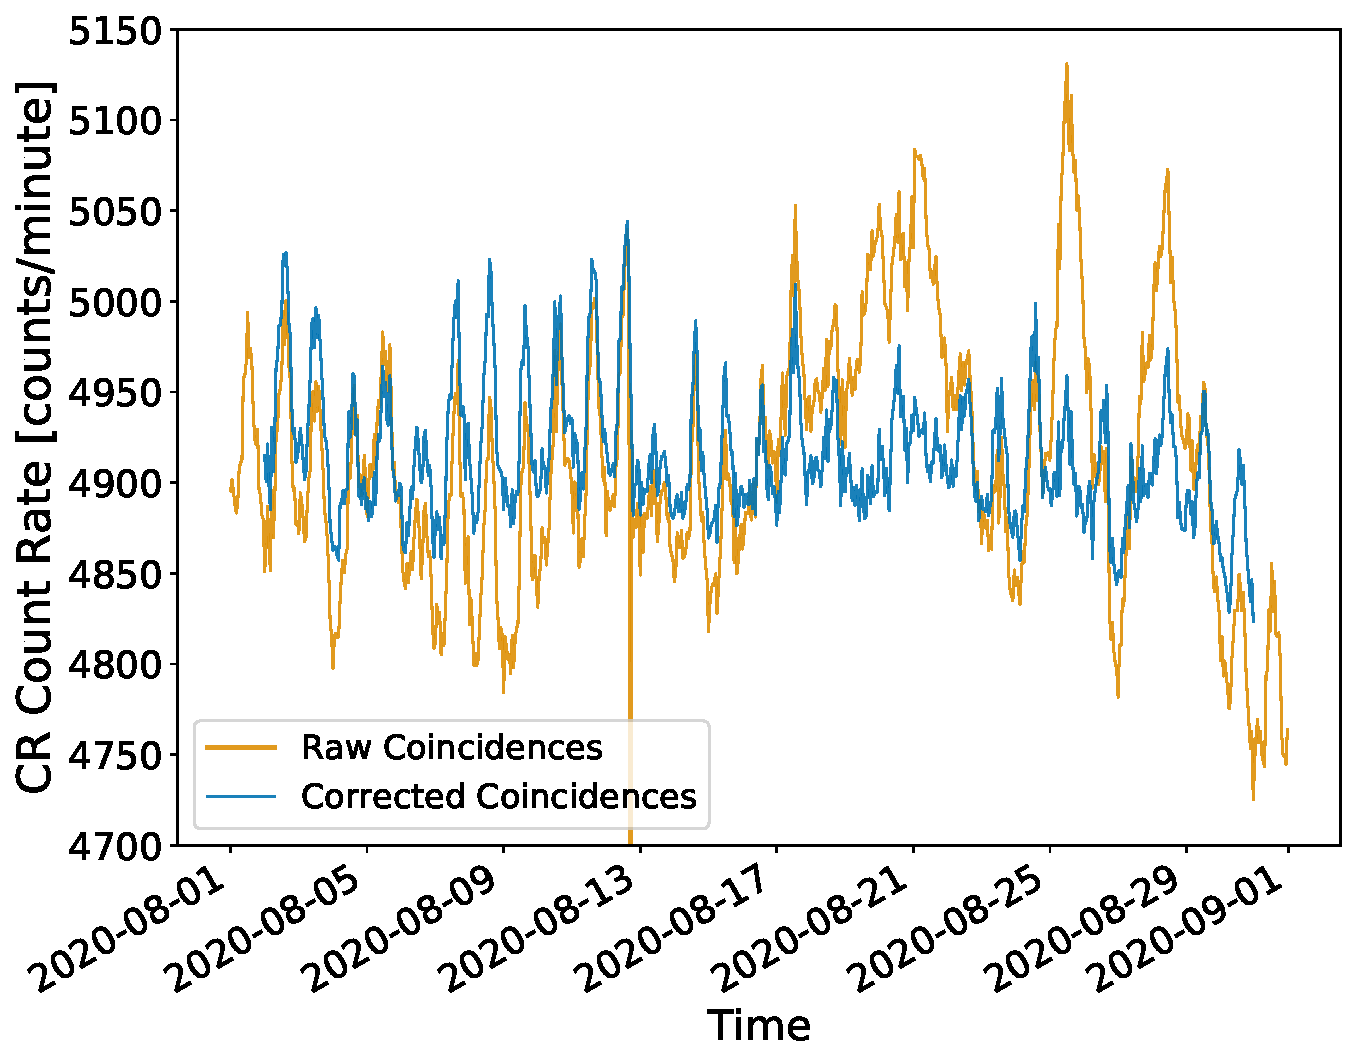
\includegraphics[width=0.7\columnwidth]{raw_vs_corrected_coincidences.pdf}
	\caption{Showing the coincidences data before (orange line) and after (blue line) the barometric correction. The hourly resampled data are over-plotted to highlight the main variation in the data.}
	\label{fig:HS_14008_corrected_coincidences}
\end{figure}


This method of barometric correction was routinely applied to coincidences data and singles data, to remove the barometric effect from the data acquired in this configuration. %However, these data were not stored on the Raspberry Pi or local servers.



%%%%%%%%%%%%%%%%%%%%%%%%%%%%%%%%%%%%%%%%%%%%%%%%%%%%%%%%%%%%%%%%%%%%%
\section{Results}\label{sec:HS_14008_results}

%%%%%%%%%%%%%%%%%%%%%%%%%%%%%%%%%%%%%%%%%%%%%%%%%%%%%%%%%%%%%%%%%%%%%
%%%%%%%%%%%%%%%%%%%%%%%%%%%%%%%%%%%%%%%%%%%%%%%%%%%%%%%%%%%%%%%%%%%%%
\subsection{Observations}\label{sec:HS_14008_observations}

From the \gls{corsika} air shower simulations performed in Chapter~\ref{chap:HiSPARC}, we predicted an approximate ground level muon rate passing through a single \gls{hisparc} detector of $\sim$85~$\upmu/\mathrm{s}$ (for non-vertical, i.e. $70^\circ$ acceptance cone simulations), and $160 \, \upmu/\mathrm{s}$ (for vertical simulations). These rates were comparable to the generally accepted, average ground level muon flux on the order of $\sim 70 \, \mathrm{m}^{-2}\,\mathrm{s}^{-1}\,\mathrm{sr}^{-1}$ \citep{cecchini_cosmic_2000, blackmore_terrestrial_2015, pereira_ground-level_2021, particle_data_group_review_2020}.

%(do this by integrating under curve, using 70-degree half-angle cone for solid angle, and area of 0.5m2)
% i.e. in python doing doing:
% where df contains the alpha and proton diff fluxes
% v = scipy.integrate.simps(df_a_v[1]+df_p_v[1], df_a_v.index.values)
% sr = 4*np.pi*(np.sin(np.deg2rad(70/2)))**2
% area = 0.5
% rate_v = v*sr*area

In Figure~\ref{fig:corrected_coinciences} we show the corrected, original coincidence data which appears to have a mean count rate of $\sim80 \, \upmu/\mathrm{s}$. In this plot we can see the diurnal effect. The diurnal effect measured here induced a variation in the \gls{cr} count between $\sim$1--2~\%, which is larger than the $\sim0.5~\%$ diurnal variation, discussed in the literature \citep{mishra_study_2007, mishra_cosmic_2008, dubey_cosmic_2016, thomas_decadal_2017}, but is significantly lower than the variation observed in the standard \gls{hisparc} events and singles data in Chapter~\ref{chap:HiSPARC}. For any given epoch, the diurnal effect can be removed, if necessary, by subtracting a smoothed time series.%, which is also shown in Figure~\ref{fig:corrected_coinciences}.

\begin{figure}[ht!]
	\centering
	%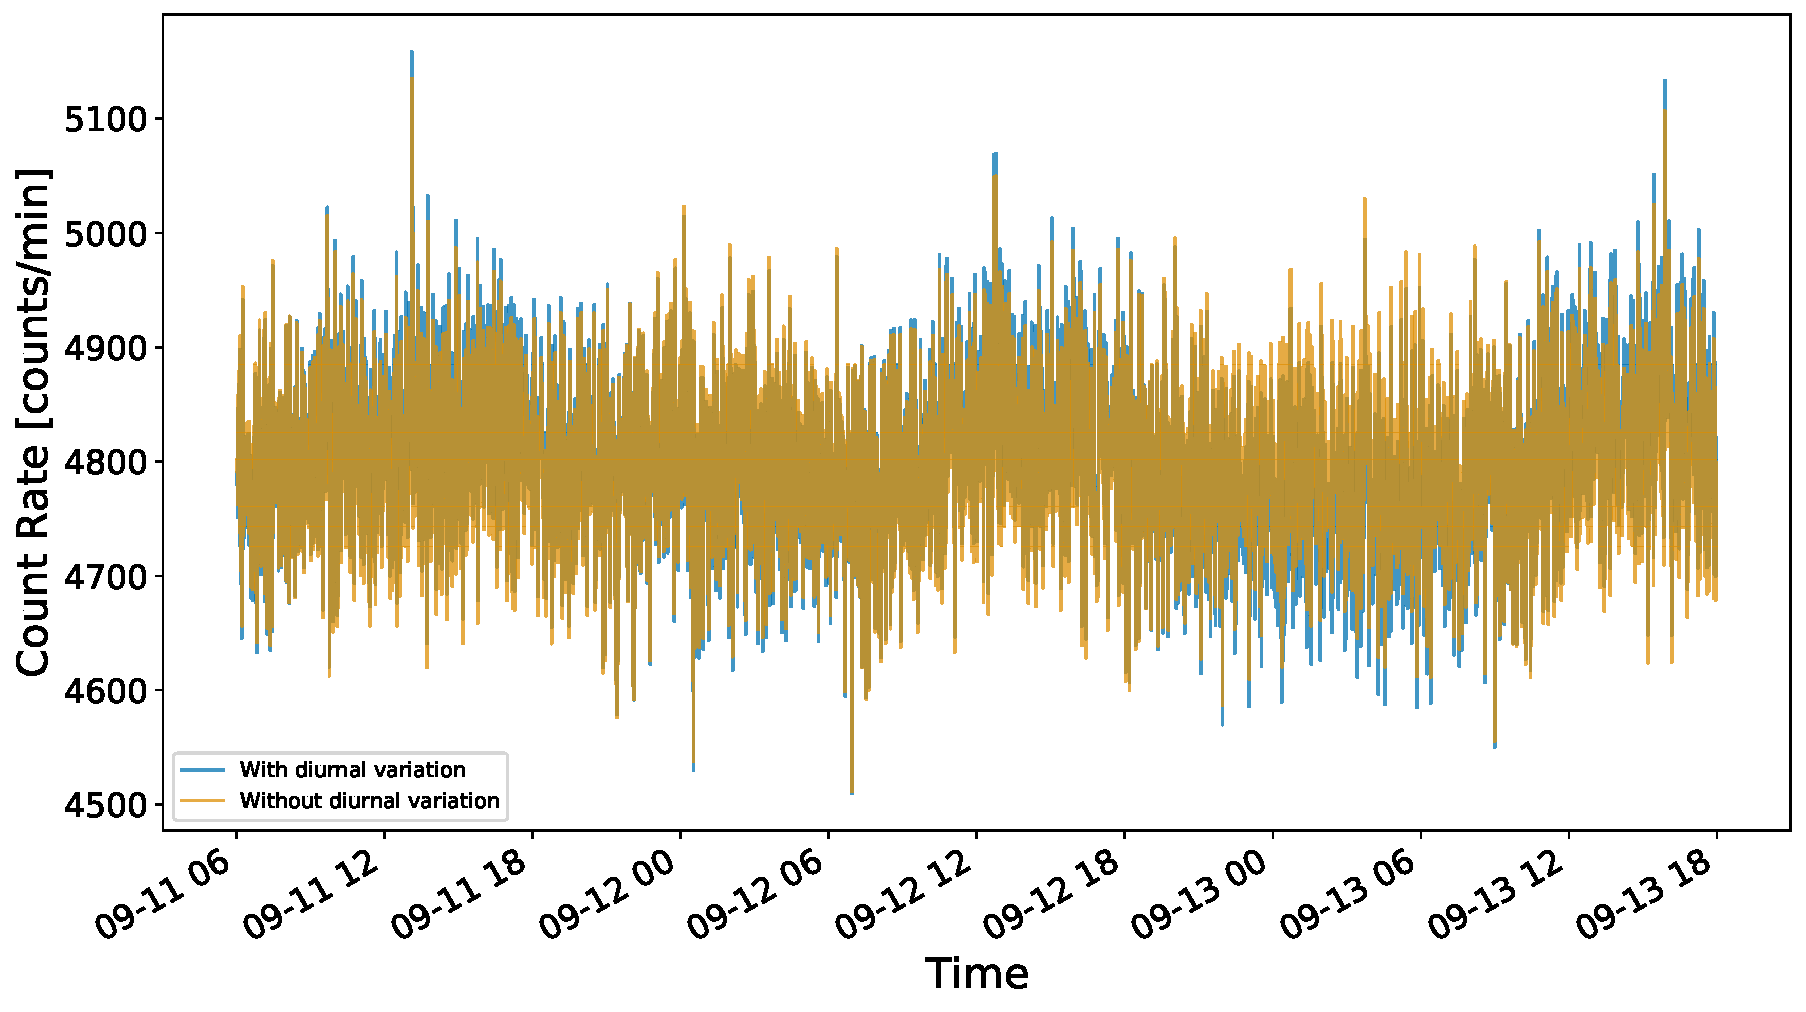
\includegraphics[width=\columnwidth]{many_day_diurnal_effect_timeseries.pdf}
	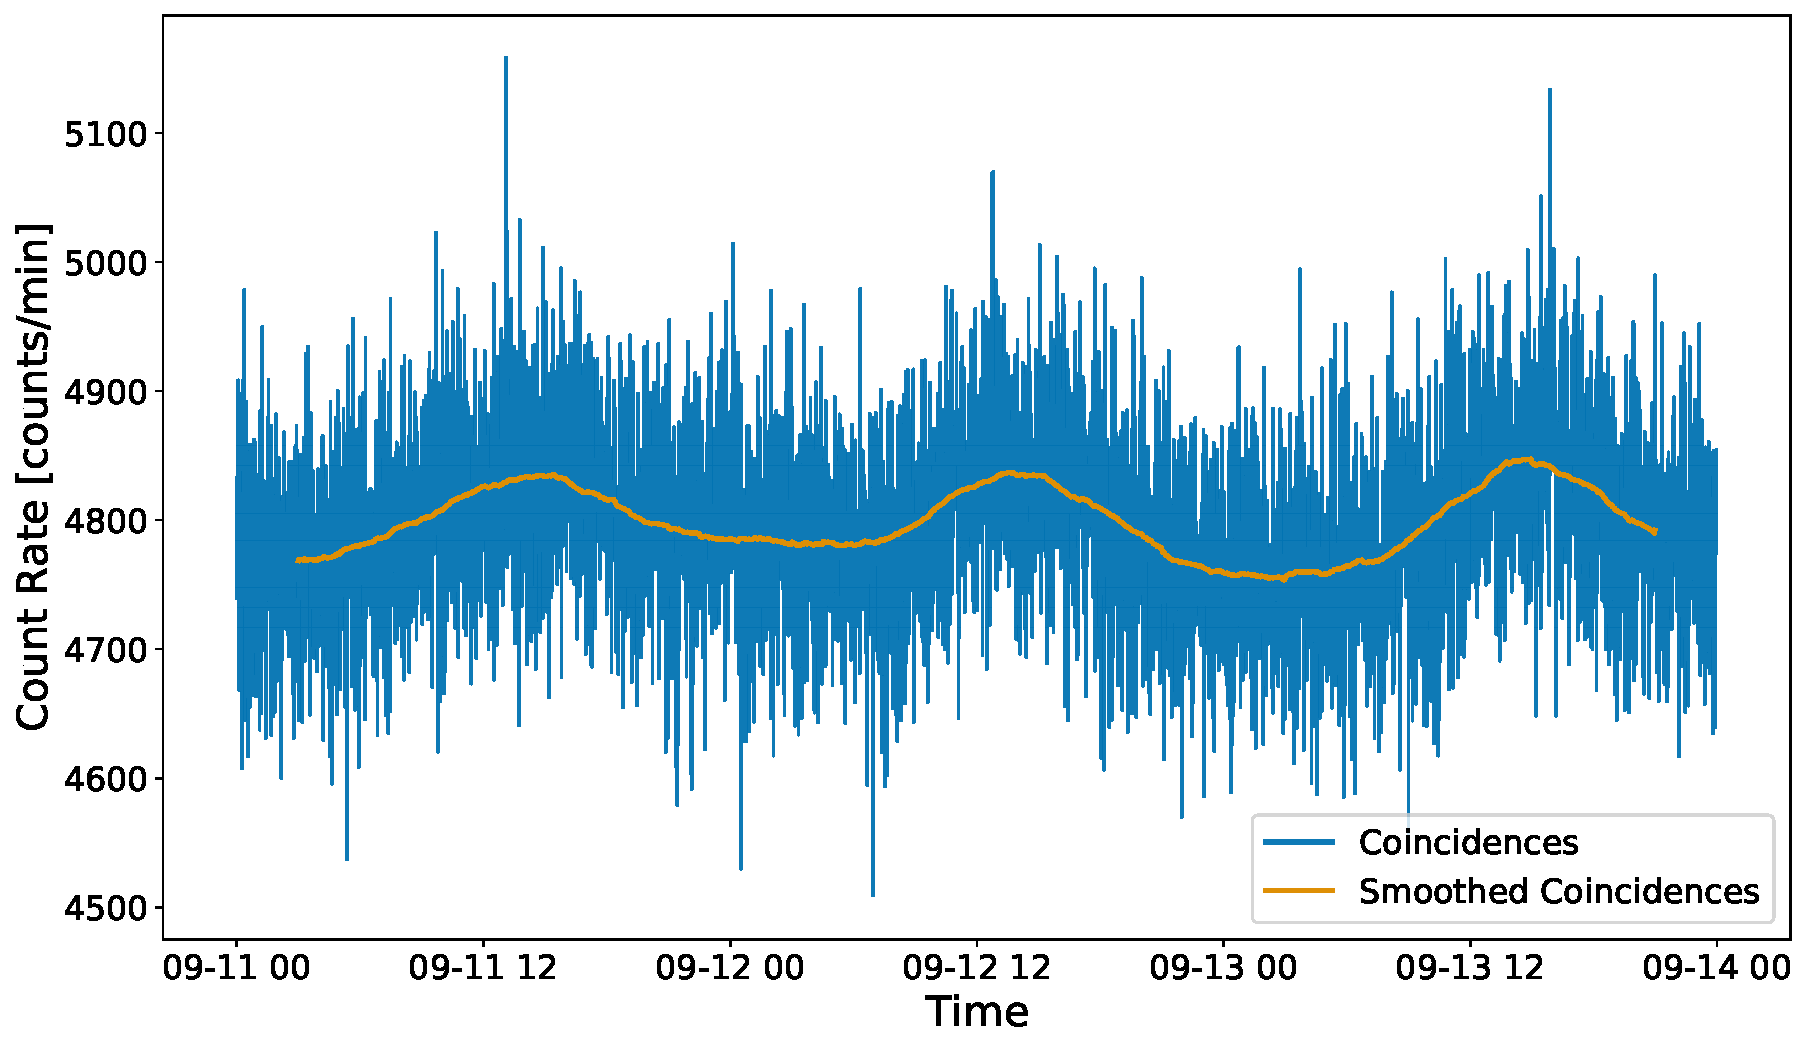
\includegraphics[width=\columnwidth]{diurnal_timeseries.pdf}
	\caption{Time series of coincidences data, corrected for atmospheric pressure. The blue line shows the corrected data displaying the diurnal variation with peaks at around midday. The orange line shows the data smoothed using a 6-hour box-car. The units of time on the x-axis are, MM-DD HH.}
	\label{fig:corrected_coinciences}
\end{figure}


As the counts follow a Poisson distribution we sampled the data using the {\verb pymc3 } \gls{nuts} extension to a \gls{hmc} sampling algorithm \citep{salvatier_probabilistic_2016} with a Poisson distribution likelihood function. This allowed us to determine the mean count rate and convergence was interrogated using the Gelman-Rubin $\widehat{R}$ diagnostic factor \citep{gelman_inference_1992} using the criteria that chains did not converge if $\widehat{R} > 1.01$. 

%The distribution of the random coincidences is shown in Figure~\ref{fig:poisson_coinciences_dist}.
%
%
%\begin{figure}[ht!]
%	\centering
%	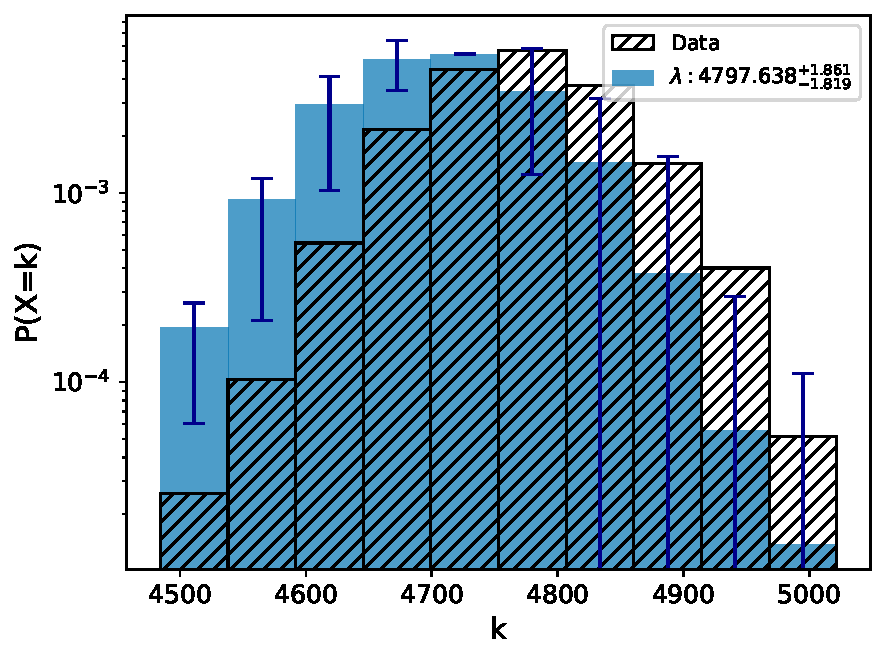
\includegraphics[width=0.9\columnwidth]{fitted_poisson.pdf}
%	\caption{Distribution of ... and Poisson distribution of the random coincidences, along with the median posterior fitted mean of the sample...}
%	\label{fig:poisson_coinciences_dist}
%\end{figure}


The median value of the posterior distribution for the mean value of the Poisson distribution of these coincidence data was $4797\pm2$~counts/min, where the uncertainties represent the $68~\%$ credible intervals either side of the median. We therefore have a count rate of $\sim80~\upmu/\mathrm{s}$ in this stacked detector configuration. This agrees remarkably well with the predicted value from the non-vertical simulations in Chapter~\ref{chap:HiSPARC}, which represents a good approximation of the true muon flux at ground level. With a count rate of $\sim$80~$\upmu/\mathrm{s}$, the Poisson noise is a rate of $\sim$9$~\upmu/\mathrm{s}$, which represents $\sim$11~\% of the signal.


These observations have used the original coincidences data, to determine the mean count rate. These data are stored only locally, but we also acquire the reduced count rates which are stored locally and separately on the \gls{hisparc} servers. The reduced coincidences data sent to the \gls{hisparc} servers use the \gls{nim} gate signal as a trigger which reduces the count rate by a factor of $\sim$100. The data stored locally were acquired slightly differently. As discussed in Section~\ref{sec:HS14008_data_acqusition}, the reduced counts (stored locally by the Python script) used the \gls{nim} counter to measure the rate of the external trigger signal (i.e. coincidences between the \gls{nim} gate signal, and the coincidences between the two \glspl{pmt}). The \gls{hisparc} events data use the trigger to read the events directly from the \glspl{pmt}. Due to the delays in the signal in the \gls{nim} crate configuration, we investigated both data sets to ensure that they did not differ. In Figure~\ref{fig:reduced_coincidences} we show a comparison between the reduced coincidences data stored locally and those recorded as events data in the \gls{hisparc} server.

%\begin{figure}[ht!]
%	\centering
%	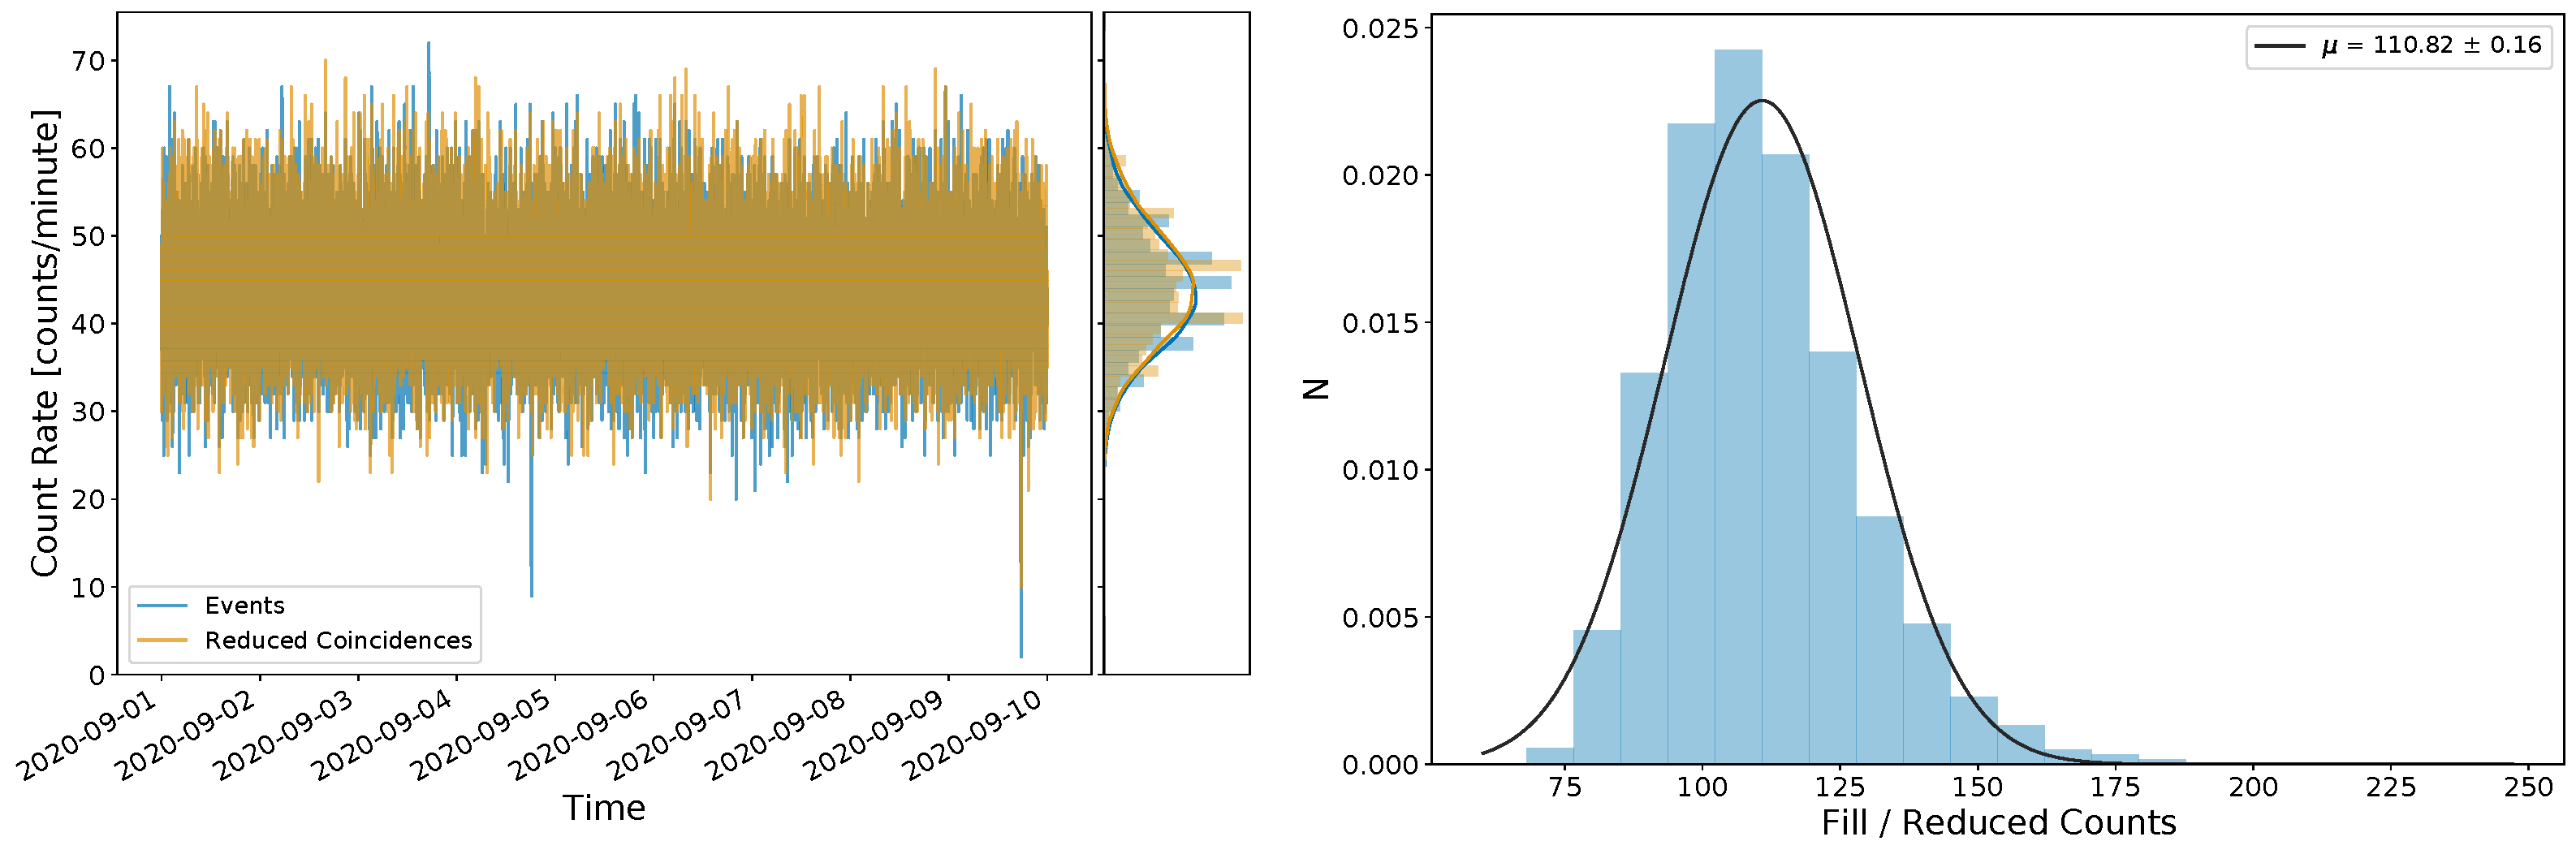
\includegraphics[width=\columnwidth]{reduced_coinc.pdf}
%	\caption{Comparison of the reduced coincidences stored locally and as events data in the HiSPARC server (left); }
%	\label{fig:reduced_coincidences}
%\end{figure}

\begin{figure}[ht!]
	\centering
	\subfloat[Time series of reduced coincidences]{
		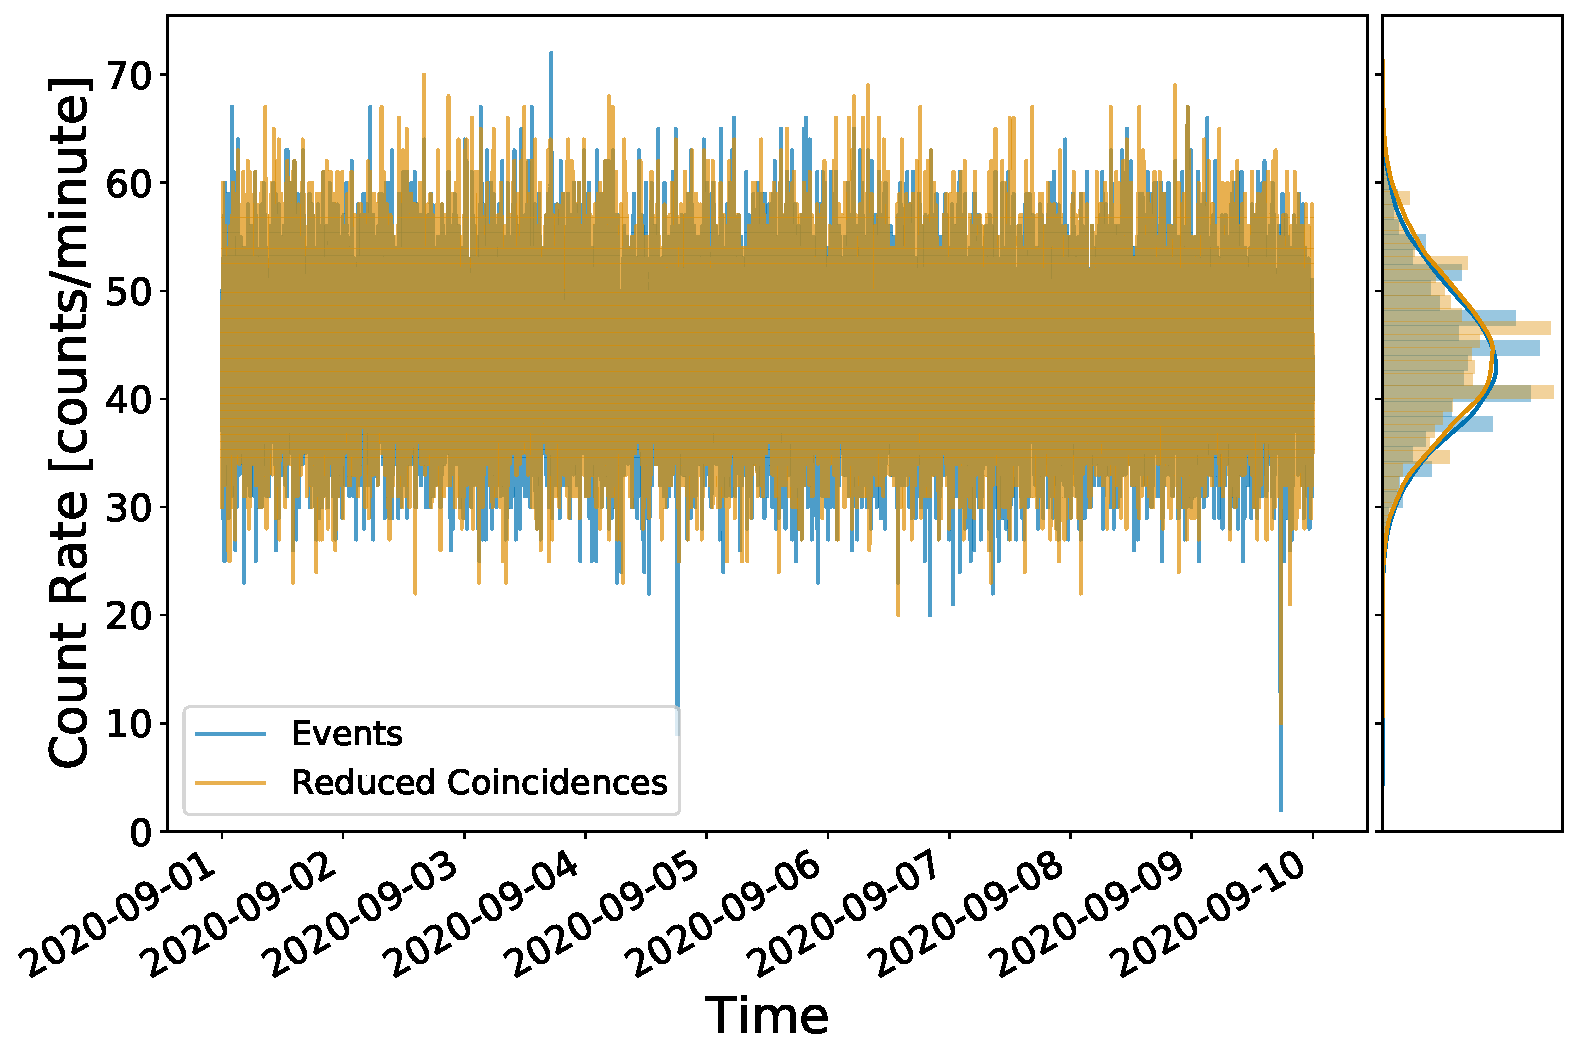
\includegraphics[width=0.52\columnwidth]{reduced_events_vs_coinc.pdf}
		\label{fig:rc1}}
	%\qquad
	\subfloat[Distribution of the ratio of original-to-reduced coincidences]{
		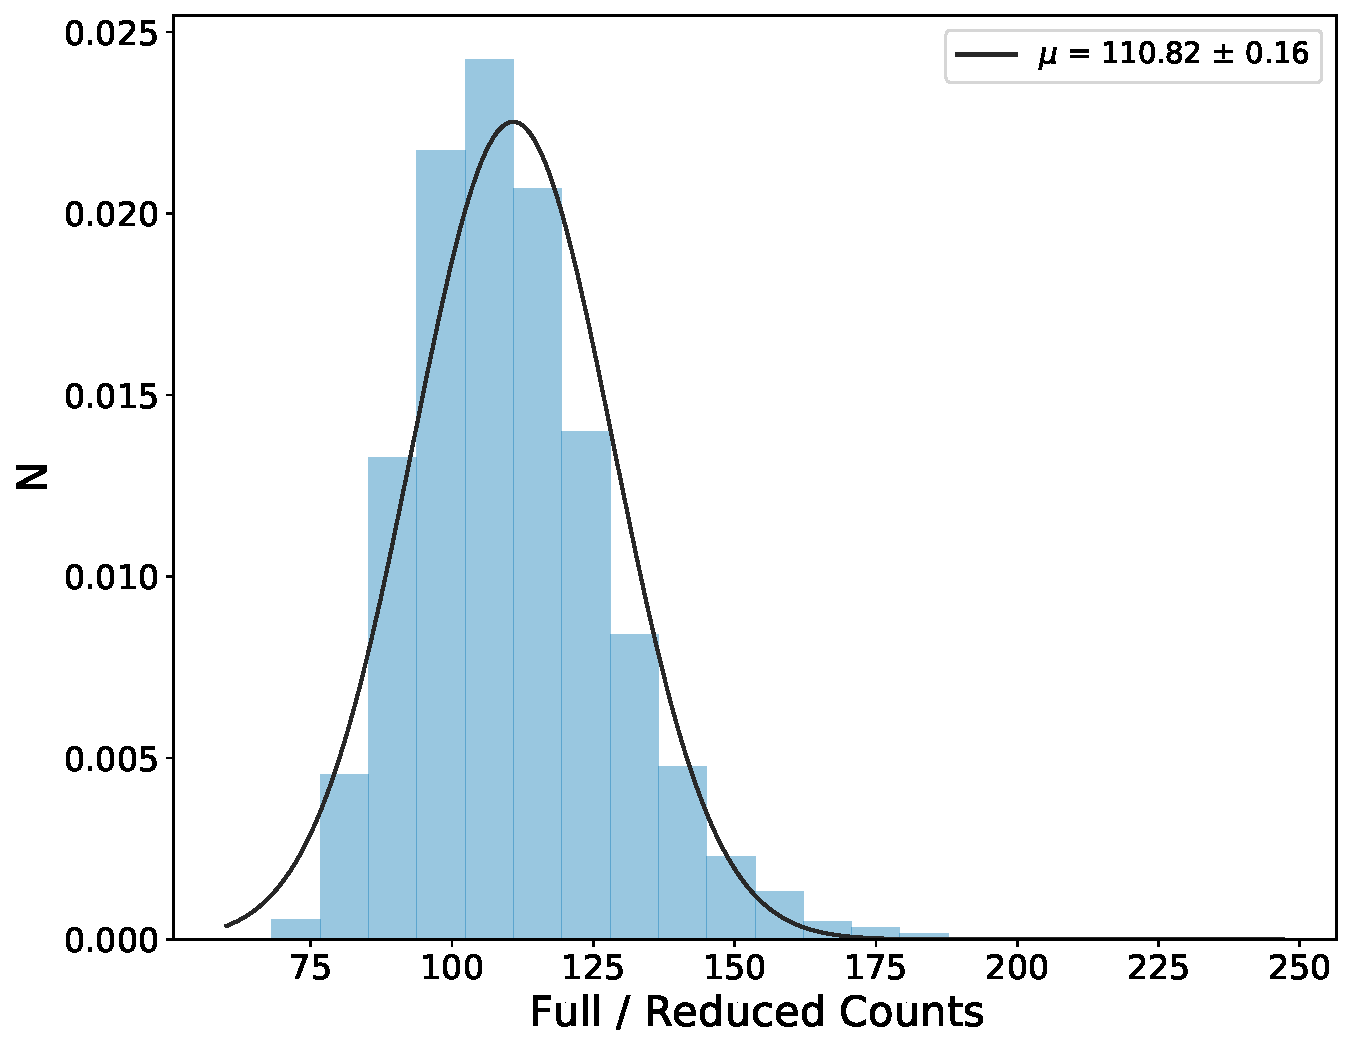
\includegraphics[width=0.44\columnwidth]{coinc_reduction_factor.pdf}
		\label{fig:rc2}} \\
	
	\caption{(a) Comparison of the reduced coincidences stored locally (orange) and as events data in the HiSPARC server (blue), where the units of time on the x-axis are, YYYY-MM-DD. (b) Distribution of the ratio of the original and reduced coincidence rates.}
	\label{fig:reduced_coincidences}
\end{figure}

The mean value of the Poisson distribution of reduced coincidences data is $\sim$44~counts/min ($\sim$0.73~$\upmu/\mathrm{s}$), which is a reduction by a factor of $\sim$110 from the original coincidences data. We can see from Figure~\ref{fig:reduced_coincidences} that both the data stored locally (reduced coincidences) and the data sent to the \gls{hisparc} server (events) are in agreement, with only the realisation of the noise being different between the data. The \gls{hisparc} data acquisition software features a pre-trigger window (duration: $1 \, \upmu\mathrm{s}$), coincidence window (duration: $1.5 \, \upmu\mathrm{s}$), and a post-trigger window (duration: $3.5 \, \upmu\mathrm{s}$). The duration of these coincidence windows means that the small delays from the \gls{nim} modules does not affect the ability of the data acquisition software to record the data from the external trigger. This verifies that the locally stored reduced coincidences data and the events data stored in the \gls{hisparc} server are measuring the same signal, with a count rate of count rate of $\sim 0.73~\upmu/\mathrm{s}$.


To understand the noise properties of this new configuration we investigated the random noise which is induced by random, spurious counts between both \glspl{pmt} which do not coincide with the passage of a muon. This was achieved by adding a delay in the signal between the two \glspl{pmt}, to ensure any coincident triggers were not due to true coincidences from the passage of a muon. By adding additional cables to the output from one \gls{pmt}, a delay of $\sim$120~ns was added between the two signals. The \gls{fwhm} of a typical pulse from the \glspl{pmt} is $\sim$25~ns, and the total duration from beginning-to-end is on the order of 100~ns \citep{van_dam_hisparc_2020}, therefore the $\sim$120~ns delay was sufficient to remove true coincidences from the observations.

The delay was added between the two PMTs for around a week and the time series of the coincidences is shown in Figure~\ref{fig:random_coinciences}. We can see that the noise is nominally $\sim 1$~count/minute.

\begin{figure}[ht!]
	\centering
	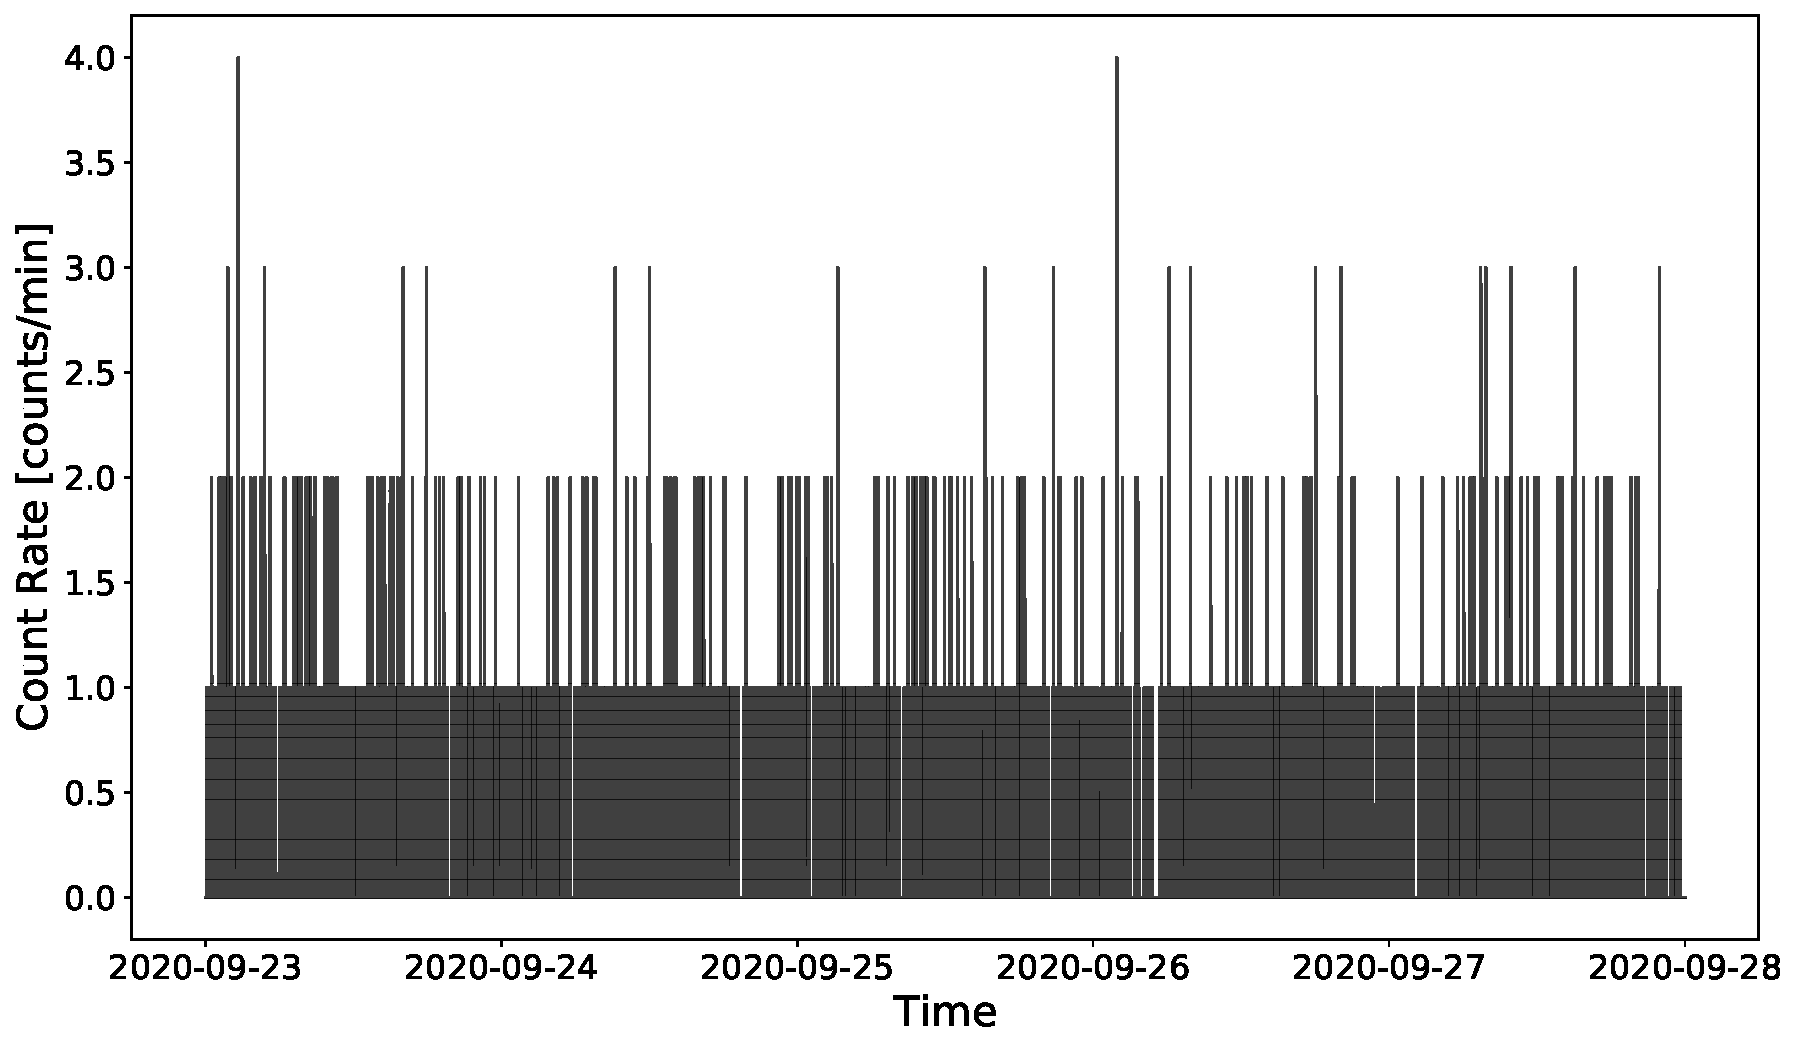
\includegraphics[width=0.9\columnwidth]{random_noise_timeseries.pdf}
	\caption{Time series of spurious coincidences data measured over five days. The units of time on the x-axis are, YYYY-MM-DD.}
	\label{fig:random_coinciences}
\end{figure}

We know the noise must follow a Poisson distribution, therefore we aimed to quantify the mean value of the spurious noise. The noise was sampled to determine the mean of the Poisson distribution using the {\verb pymc3 } \gls{nuts} extension to a \gls{hmc} sampling algorithm \citep{salvatier_probabilistic_2016}. Convergence was interrogated using the Gelman-Rubin $\widehat{R}$ diagnostic \citep{gelman_inference_1992} factor using the criteria that chains did not converge if $\widehat{R} > 1.01$. The distribution of the random coincidences is shown in Figure~\ref{fig:random_coinciences_dist}.

\begin{figure}[ht!]
	\centering
	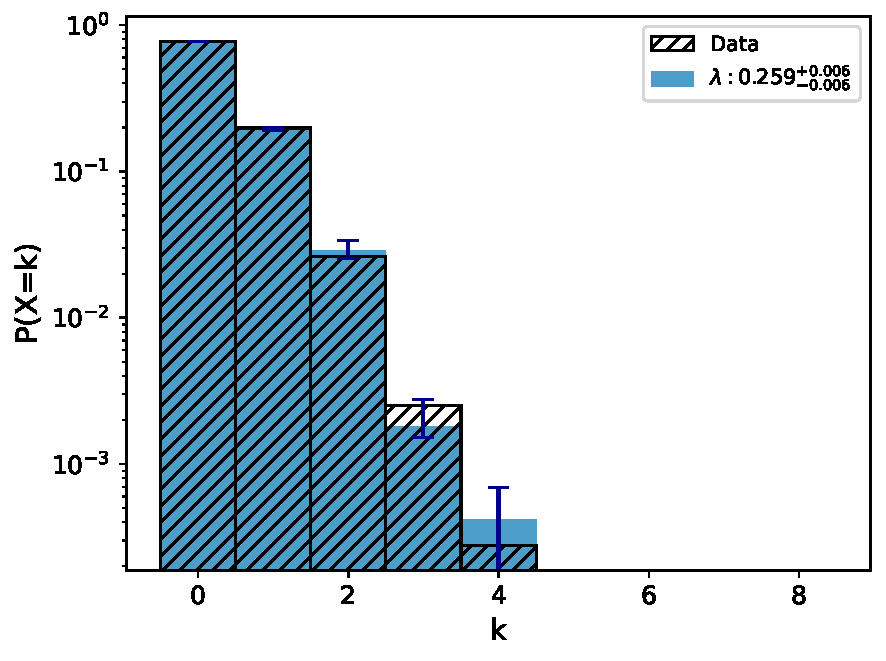
\includegraphics[width=0.8\columnwidth]{random_noise_fitted_poisson.pdf}
	\caption{Distribution plot of the random coincidences data (hatched bars), and probability mass function of a Poisson distribution with mean equal to the median value of the posterior distribution after sampling (blue bars). Blue error bars represent the $68 \%$ credible intervals either side of the median.}
	\label{fig:random_coinciences_dist}
\end{figure}

The median value of the sampled posterior of the mean value of the Poisson distribution of random coincidence is $0.259 \pm 0.006$~counts/min, where the uncertainties represent the $68 \%$ credible intervals either side of the median. This represents a low level of noise; under this Poisson likelihood function the probability of no noise is $\sim 77 \%$, 1~count/minute is $\sim 20 \%$, and over 2~counts/minute is $< 3 \%$.

It is also important to note that in Figure~\ref{fig:random_coinciences}, there is no obvious diurnal pattern in the signal. This shows that as the \gls{pmt} thermal noise increases around midday, which we see manifesting in the singles data, the increased thermal noise does not manifest in the spurious coincidences between both \glspl{pmt}. This is important as it highlights that in this stacked detector configuration we have maximised our ability to observe single muons whilst reducing the effects of diurnal, thermally induced noise, which motivated not correcting for the weak correlation between the temperature of the \glspl{pmt} and the coincidences data.



%%%%%%%%%%%%%%%%%%%%%%%%%%%%%%%%%%%%%%%%%%%%%%%%%%%%%%%%%%%%%%%%%%%%%
%%%%%%%%%%%%%%%%%%%%%%%%%%%%%%%%%%%%%%%%%%%%%%%%%%%%%%%%%%%%%%%%%%%%%
\subsection{Comparison with Neutron Monitors}\label{sec:HS_14008_vs_Kiel}

It is useful to compare the data from this new \gls{hisparc} station to an existing \gls{nm} detector in the \gls{gnmn} \citep{mishev_current_2020}, as \glspl{nm} are one of the most widely used sources of data for monitoring space weather. Unfortunately, there were no space weather events from the beginning of \gls{hisparc} station 14008 operation to the time of writing; however, we still show a comparison to a nearby \gls{nm} station. %as this can highlight whether any confirmed space weather events using the \gls{gnmn} have been observed with this new instrument.

The Kiel \gls{nm} station, in Germany, used in Chapter~\ref{chap:HiSPARC} had suffered difficulties with data consistency during this epoch, therefore another station was used in the analysis here. We chose to analyse the \gls{nm} count rate at Dourbes, which is located in Belgium and \textit{is} the nearest \gls{nm} to the \gls{hisparc} network, at $\sim$525~km away from station 14008 in Birmingham. The properties of the Dourbes station are: $R_C$=3.18~GV, Altitude=225~m, Latitude=$50.10^{\circ}$N, Longitude=$4.59^{\circ}$E \citep{nmdb_nmdb_nodate}. In Figure~\ref{fig:14008_vs_DRBS}, a comparison is shown between the corrected \gls{hisparc} coincidences data and the Dourbes \gls{nm} station during November 2020.

\begin{figure}[ht!]
	\centering
	\subfloat[HS 14008 vs Dourbes (offset)]{
		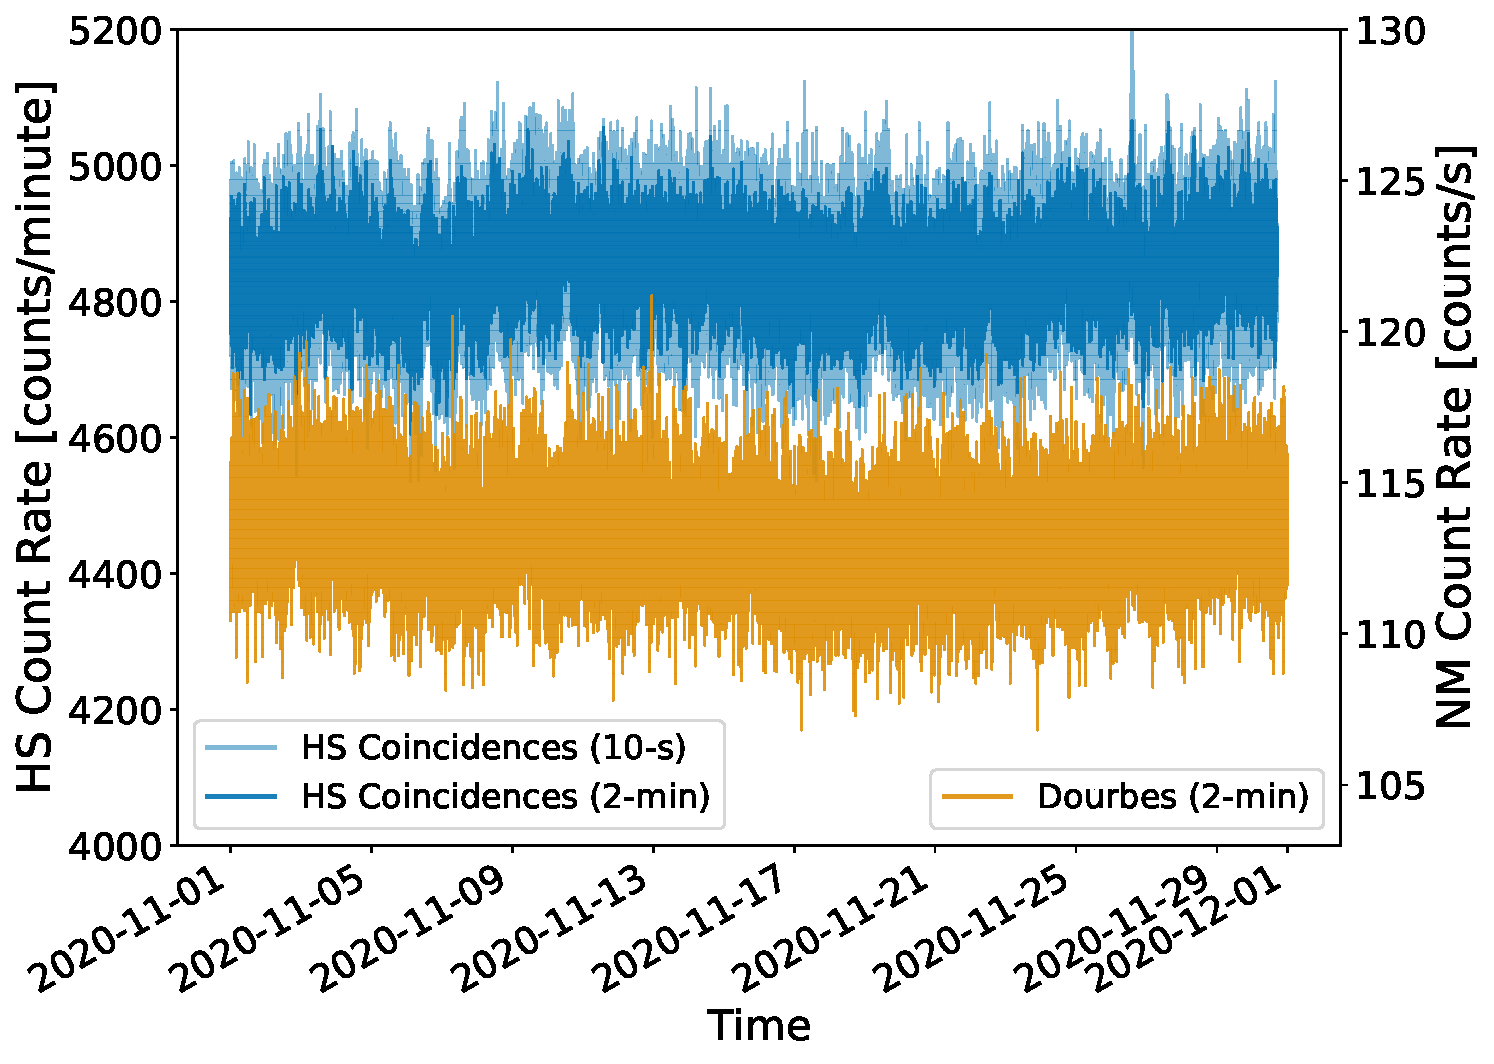
\includegraphics[width=0.48\columnwidth]{HS14008_vs_DRBS.pdf}
		\label{fig:14008vsDRBS_1}}
	%\qquad
	\subfloat[HS 14008 vs Dourbes (overlay)]{
		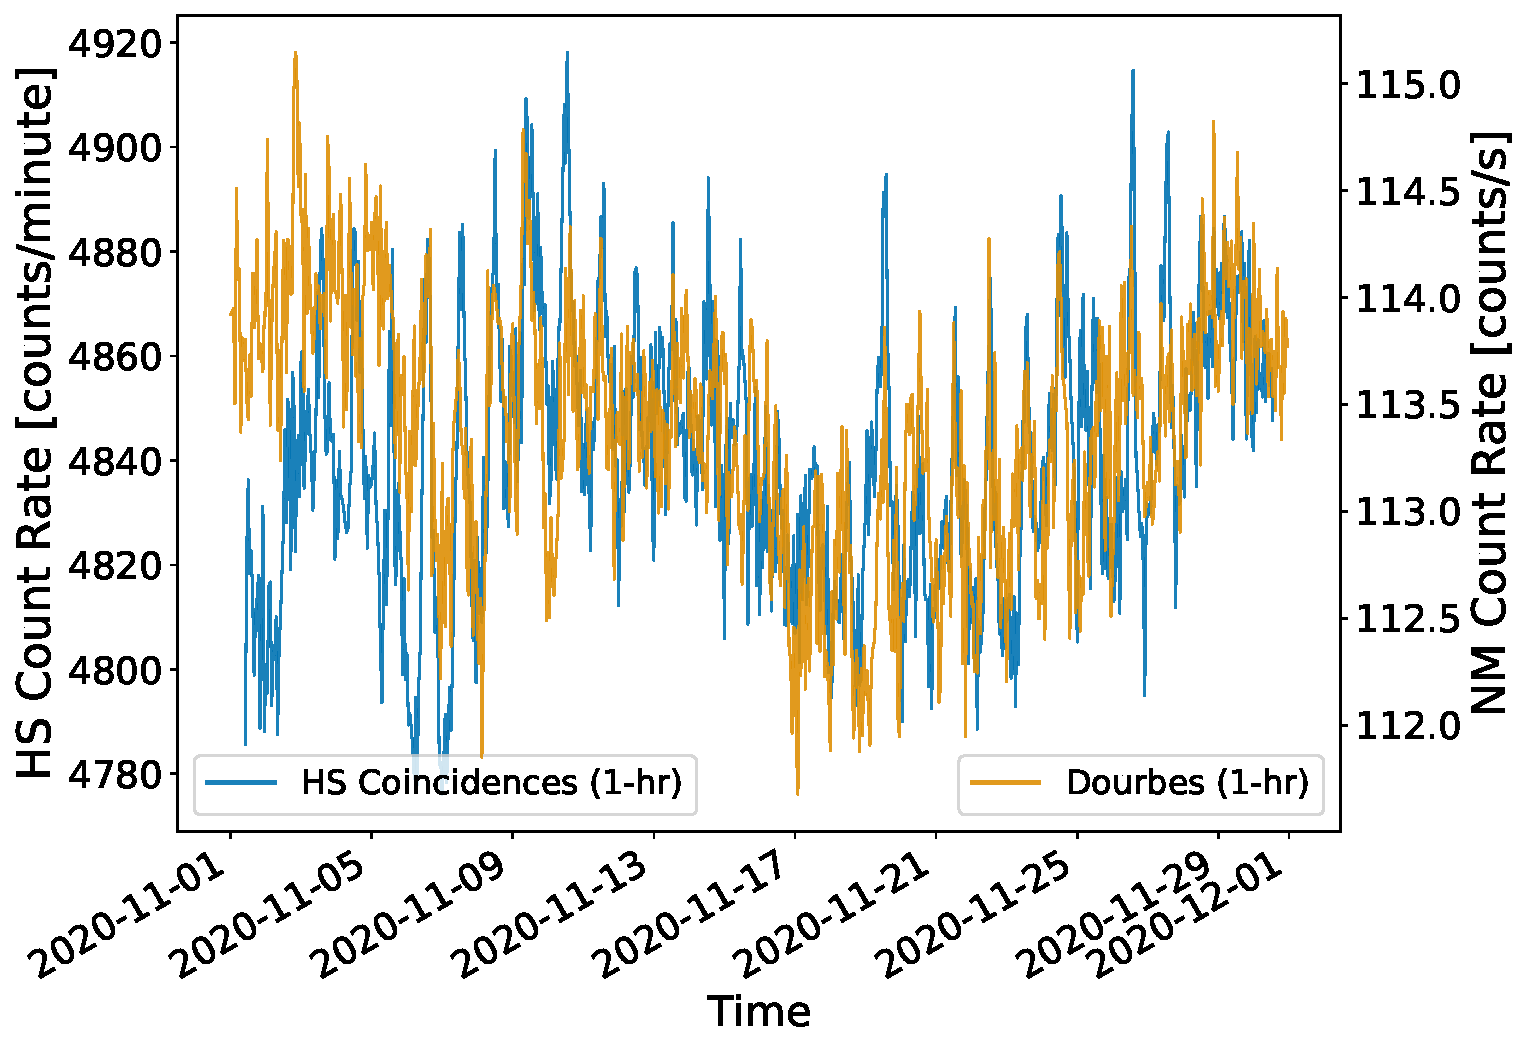
\includegraphics[width=0.48\columnwidth]{HS14008_vs_DRBS_overlay.pdf}
		\label{fig:14008vsDRBS_2}} \\

	
	\caption{A comparison between the corrected HiSPARC station 14008 coincidences data (blue) and the pressure corrected neutron monitor data measured at the Dourbes NM station, Belgium. (a) Shows the two data sets offset and (b) overlayed hourly-averaged data, showing the similarities between the two data sets. Units of time on the x-axis are, YYYY-MM-DD.}
	\label{fig:14008_vs_DRBS}
\end{figure}


The plots in Figure~\ref{fig:14008_vs_DRBS} show a good visual agreement between the two detectors. Despite a good visual agreement, the Pearson correlation coefficient was $\rho \sim 0.08$, highlighting that there was no correlation between the two stations, at the 2-minute level. When resampling the data to 1-hour and 1-day the correlation increased to $\rho \sim 0.40$ and $\rho \sim 0.41$, respectively. This showed a weak, low frequency correlation between the two stations. This weak correlation showed the two stations monitor approximately the same background \gls{cr} signal, which is relatively flat as the solar activity is low, therefore contributions from \glspl{scr} are low. At the 2-minute level, the near-zero correlation demonstrates that the variations in the two signals are dominated by noise and there was no covarying signal.

This comparative analysis should be continually monitored, and particularly used as a reference when any space weather events are recorded with the \gls{gnmn}. As it is the closest \gls{nm} to the \gls{hisparc} 14008 detector in Birmingham, it is useful to continue using the Dourbes \gls{nm} station, but also to incorporate the use of data from the Kiel \gls{nm} station, when issues with data quality are resolved. Near the maximum of Solar Cycle 25, expected 2023--2026, and likely to arrive in 2025 \citep{mcintosh_overlapping_2020, pesnell_lessons_2020}, we would expect the correlation to grow as the number of \glspl{sep} increases. It is therefore important that this configuration of \gls{hisparc} detector is maintained until at least 2026, to ensure a complete study is performed when solar activity and space weather activity is high.


%%%%%%%%%%%%%%%%%%%%%%%%%%%%%%%%%%%%%%%%%%%%%%%%%%%%%%%%%%%%%%%%%%%%%
\subsection{Single Station Space Weather Uses}\label{sec:HS_14008_single_sims}

Simulations of artificial data were performed to determine the magnitude of \glspl{gle} that may be observed in this new station configuration, as described in Section~\ref{sec:HS_14008_method_obs}. We have shown the \gls{hisparc} 14008 station has a background, mean count rate, $\lambda\sim80~\upmu/\mathrm{s}$, and a noise of $\sigma\sim0.26~\upmu/\mathrm{min}$ (i.e. $\sim0.004~\upmu/\mathrm{s}$). These were used as inputs to the simulations, where \glspl{gle} were simulated with amplitudes of: $1.0\%$--$5.0\%$, in intervals of $0.5\%$. In addition, we simulated \glspl{gle} with amplitudes of: $7.5\%$ and $10.0\%$. The artificial data were created using the method in Appendix~\ref{app:GLE_sims} and the statistics tests performed on the resultant data.

Running several iterations, it was possible to analyse the statistics for each amplitude of \gls{gle}, compared to the background signal/mean count rate of the detector, without a \gls{gle}. An example of the output from the statistical tests on a single iteration is shown in Figure~\ref{fig:simulated_data_stats}, for a $10 \%$ \gls{gle} magnitude. Table~\ref{tab:HS_14008_sims_zeros} shows the average number of measurements exceeding the various thresholds by chance for simulations without any injected \glspl{gle}.


\begin{figure}[ht!]
	\centering
	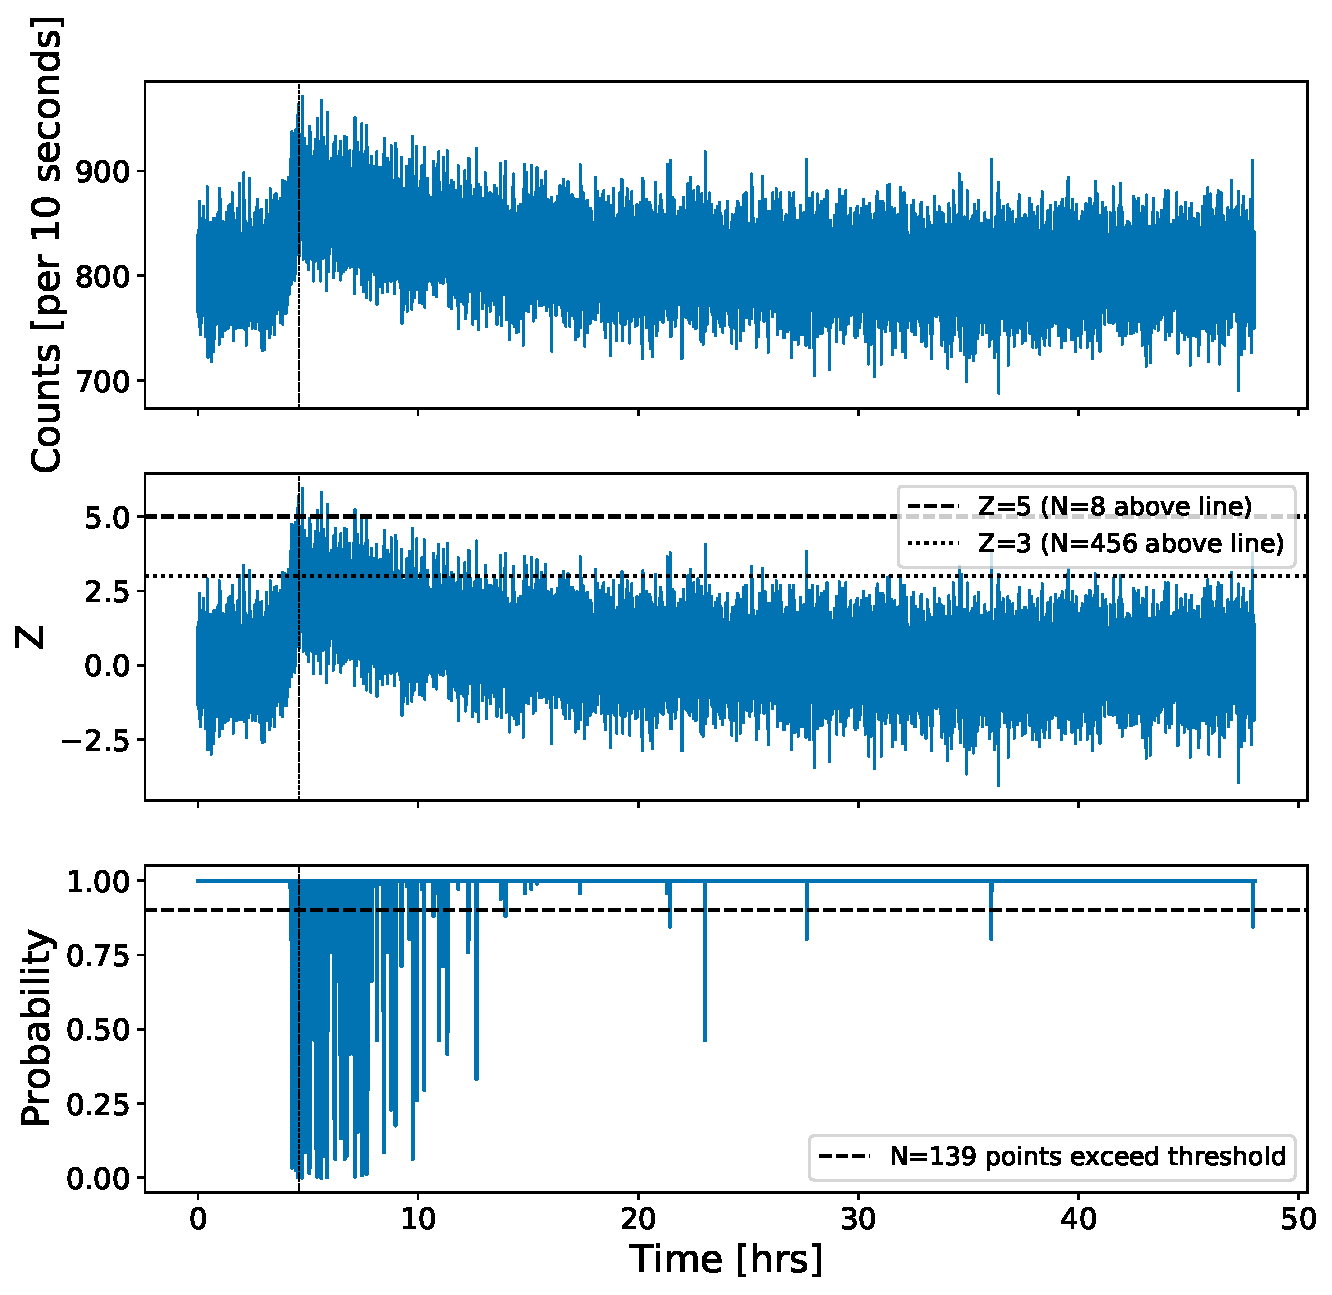
\includegraphics[width=0.9\columnwidth]{simulated_data_stats.pdf}
	\caption{Single realisation of a simulation with a $10\%$ \gls{gle} magnitude. Top panel shows the raw, artificial data from the simulation, with a 10-second cadence. Middle panel shows the number of measurements exceeding the $Z=3$ and $Z=5$ thresholds. The $Z=3$ and $Z=5$ thresholds are depicted as dotted and dashed lines, respectively. Bottom panel shows the number of points exceeding the $p = 10 \%$ threshold in the binomial test, where a low probability value indicates a high chance the measurement is not statistical fluctuation. The dashed line shows the $p = 10 \%$ threshold.}
	\label{fig:simulated_data_stats}
\end{figure}

\vspace{1em}

\begin{table}[ht!]
	\begin{center}
		\caption{Median number of excessive measurements in the artificial data with no injected GLEs. The values were acquired from 1000 iterations of simulated data, performing each of the three statistical tests: binomial, $Z=3$, and $Z=5$, for the 10-s cadence data and averaging over 1-minute and 5-minutes. All uncertainties correspond to the 68\% credible intervals either side of the median.}
		\label{tab:HS_14008_sims_zeros}
		\begin{tabular}{c c c c}
			\hline 
			{} & \multicolumn{3}{c}{\bf No. excessive measurements} \\ 
			{\bf Data cadence} & {\bf Binomial} & {\bf $\mathbf{Z=3}$} & {\bf $\mathbf{Z=5}$}  \\ 
			\hline 
			10-second & $2^{+2}_{-1}$ & $27^{+6}_{-5}$ & $0 \pm 0$ \\ 
			1-minute & $0^{+1}_{-0}$ & $4 \pm 2$ & $0 \pm 0$ \\ 
			5-minute & $0 \pm 0$ & $1 \pm 1$ & $0 \pm 0$ \\ 
			\hline 
		\end{tabular} 
	\end{center}
\end{table}
%
%10-second & $2^{+2}_{-1}$ & $27^{+6}_{-5}$ & $0 \pm 0$ \\ 
%1-minute & $2^{+1}_{-2}$ & $4 \pm 2$ & $0 \pm 0$ \\ 
%5-minute & $1 \pm 1$ & $1 \pm 1$ & $0 \pm 0$ \\ 
%
\vspace{1em}

Table~\ref{tab:HS_14008_sims_zeros} shows what one sees (on average) by chance, with no \glspl{gle} present. In the case of the binomial test on the raw, 10-second cadence data, we found there was a 10\% chance of observing $2^{+2}_{-1}$ or more measurements over the threshold, by chance, when using $N=720$ points in equation~(\ref{eq:poisson_binom_CDF}) (i.e. $\sim$2~hours). In Section~\ref{sec:HS_14008_method_obs}, we showed, on average, we would expect to measure approximately 2.4 points exceeding the threshold due to statistical fluctuations, in a 48-hour period; therefore the value in Table~\ref{tab:HS_14008_sims_zeros} agrees with the expected number. In the event of a \gls{gle}, we could claim a significant observation using the binomial threshold if we observed over $\sim$12 measurements (i.e. as there is a probability of $\sim8.5\times10^{-7}$ to observe random instances across the 24 independent realisations, which is comparable with the 5$\sigma$ level). In particular, with the binomial test, we expect measurements of a \gls{gle} to give several excessive points close together, at the time of the \gls{gle}, and not scattered over the 48-hour period. %This value of $N$ was chosen as it is approximately the average \gls{fwhm} for \glspl{gle} \citep{strauss_pulse_2017}. In a 48-hour window, observing with a cadence of 10-seconds, we have $n=17280$ total points; however, using $N=720$ gives $n/N\approx24$ independent time-windows to test. 

These results therefore allow us to judge whether there is any potential significance in a given data set, depending on how the number of measurements exceeding the thresholds compares to the values in Table~\ref{tab:HS_14008_sims_zeros}. For example, in Figure~\ref{fig:simulated_data_stats}, there were 43 points exceeding the $10 \%$ binomial limit, and 154 and 3 points above the $Z=3$ and $Z=5$ limits, respectively. This indicated the existence of significance in the data, in which a \gls{gle} was injected with a magnitude of 10\%. On closer inspection one can see the grouping of the number of points exceeding each of the thresholds where the event occurred, at $\sim$5~hours. 

%With artificial data, we used the values in Table~\ref{tab:HS_14008_sims_zeros} to determine whether there existed a possible event in the data, and closer inspection of the statistics tests verified or excluded the existence of a true event. We ran several iterations of these tests to build up a picture of the \gls{gle} magnitudes we could expect to observe.

With artificial data, over a given two-day period, we can say that any epoch with a number of excessive points greater than these values can be treated as statistically of interest. We expect that any measurements which exceed the $Z=5$ threshold should clearly be treated as a significant event claim, as within two days of artificial background data, we observed no random fluctuations in the noise exceeding this level. In addition, we see that there is a large difference in the number of measurements exceeding the $Z=3$ threshold between the raw, 10-s data to 5-minute averaged data. We can be confident of claiming a statistically compatible or significant event if the number of excessive measurements exceeds 3- or 5-$\sigma$. %Finally, in the case of the binomial test, the average number of statistically significant fluctuations in the noise exceeding the $10 \%$ threshold is in the range $\sim 2-4$ in two days of data.

%The results in Table~\ref{tab:HS_14008_sims_zeros} provide the expected number of statistically significant fluctuations in the noise for each test method applied to the raw and resampled data. For a particular two day observation, we can say that any epoch with statistically significant peaks in excess of these values can be treated as statistically significant, and likely that there was a space weather event. We expect that any measurements which exceed the $Z=5$ should clearly be treated as a significant event claim, as within two days of artificial background data, we observed no random fluctuations in the noise exceeding this level. In addition, we see that there is a large difference in the number of measurements exceeding the $Z=3$ threshold between the raw, 10-s data to 5-minute averaged data. We can be confident of observing a true event if the number of significant measurements exceeds $\sim 33$, $\sim 6$, and $\sim 2$, for the raw data, 1-minute averaged data, and 5-minute averaged data, respectively. Finally, in the case of the binomial test, the average number of statistically significant fluctuations in the noise exceeding the $10 \%$ threshold is in the range $\sim 2-4$ in two days of data. We expect that the binomial method is a good measure of the existence of a true event, due to the consistency of the sensitivity, regardless of averaging over the data. 


For each \gls{gle} magnitude we ran 1000 iterations of the simulations and were able to average over the number of excessive measurements for a given \gls{gle} magnitude. In each simulation, the rise and decay times of the \glspl{gle} were randomly sampled (see Appendix~\ref{app:GLE_sims}). This was done for the raw, 10-s cadence data and further simulations were performed for 1-minute averaging and 5-minute averaging. To summarise the results of all the simulations, Figure~\ref{fig:single_HS14008_sims} shows the average number of cadences with excessive measurements against the simulated \gls{gle} magnitude for the 10-s cadence observations, 1-minute and 5-minute averages. The horizontal, dashed lines show the median number of points due to statistical fluctuations, i.e. without an injected \gls{gle}, and the horizontal, dotted lines represent the $68 \%$ credible intervals either side of the median. Each point shows the median number of excessive observations for different \gls{gle} magnitudes, also with error bars representing the $68 \%$ credible intervals either side of the median.


\begin{figure}[!htbp!]
	\centering
	\subfloat[10-s cadence simulation]{
		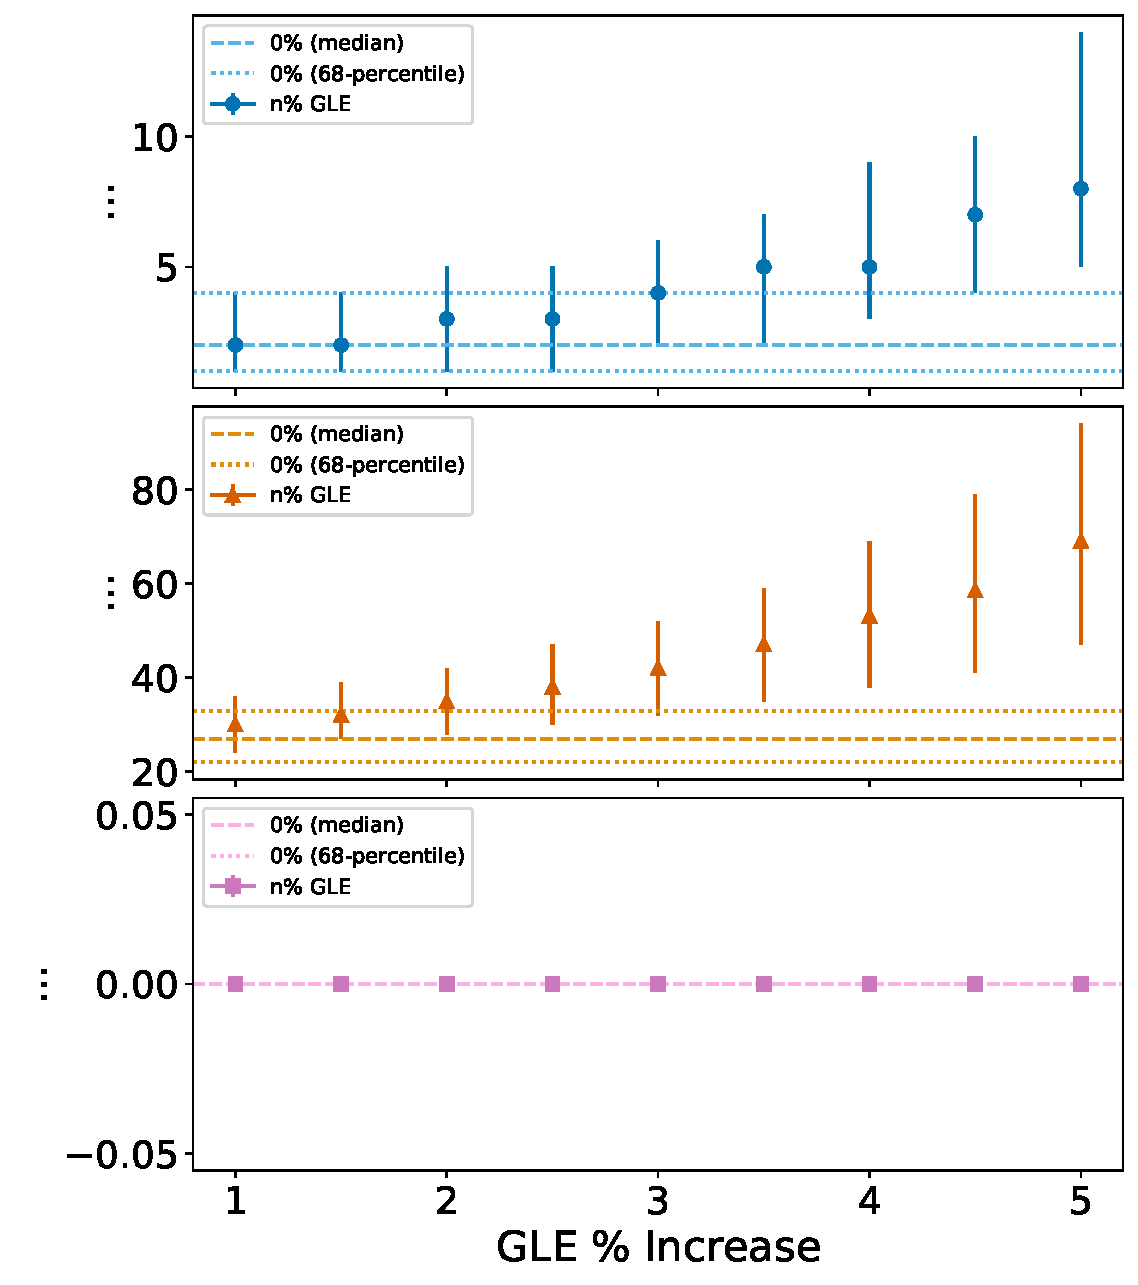
\includegraphics[width=0.48\columnwidth]{HS_14008_sims_plot_0rebin.pdf}
		\label{fig:single_sims_0min_rebin}}
	%\qquad
	\subfloat[1-minute averaging]{
		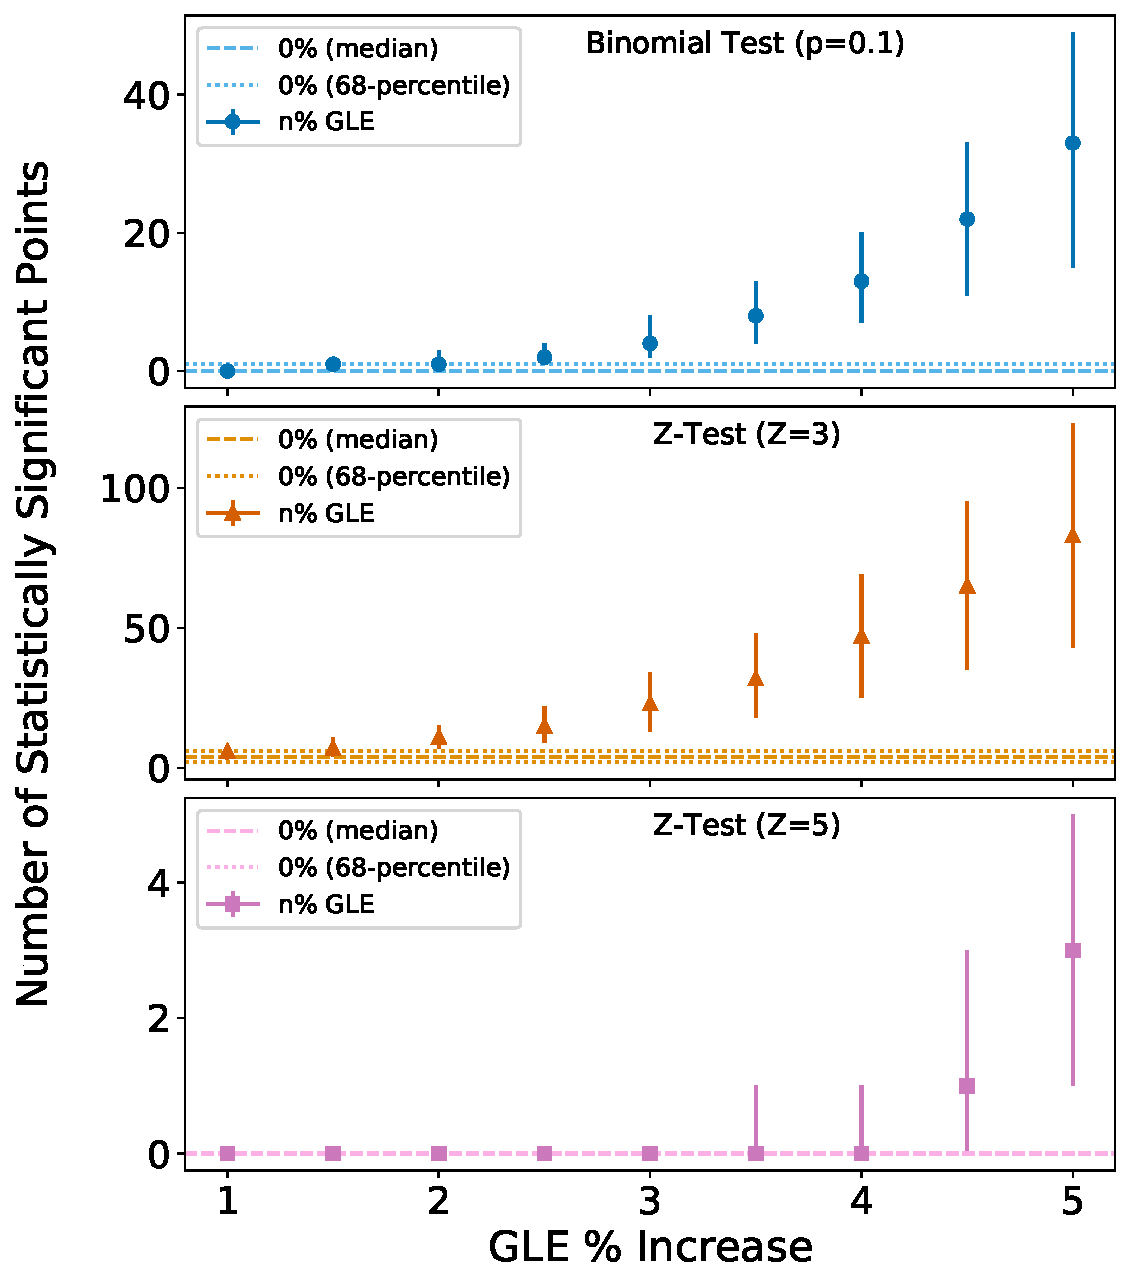
\includegraphics[width=0.48\columnwidth]{HS_14008_sims_plot_1rebin.pdf}
		\label{fig:single_sims_1min_rebin}} \\
	%\qquad
	\subfloat[5-minute averaging]{
		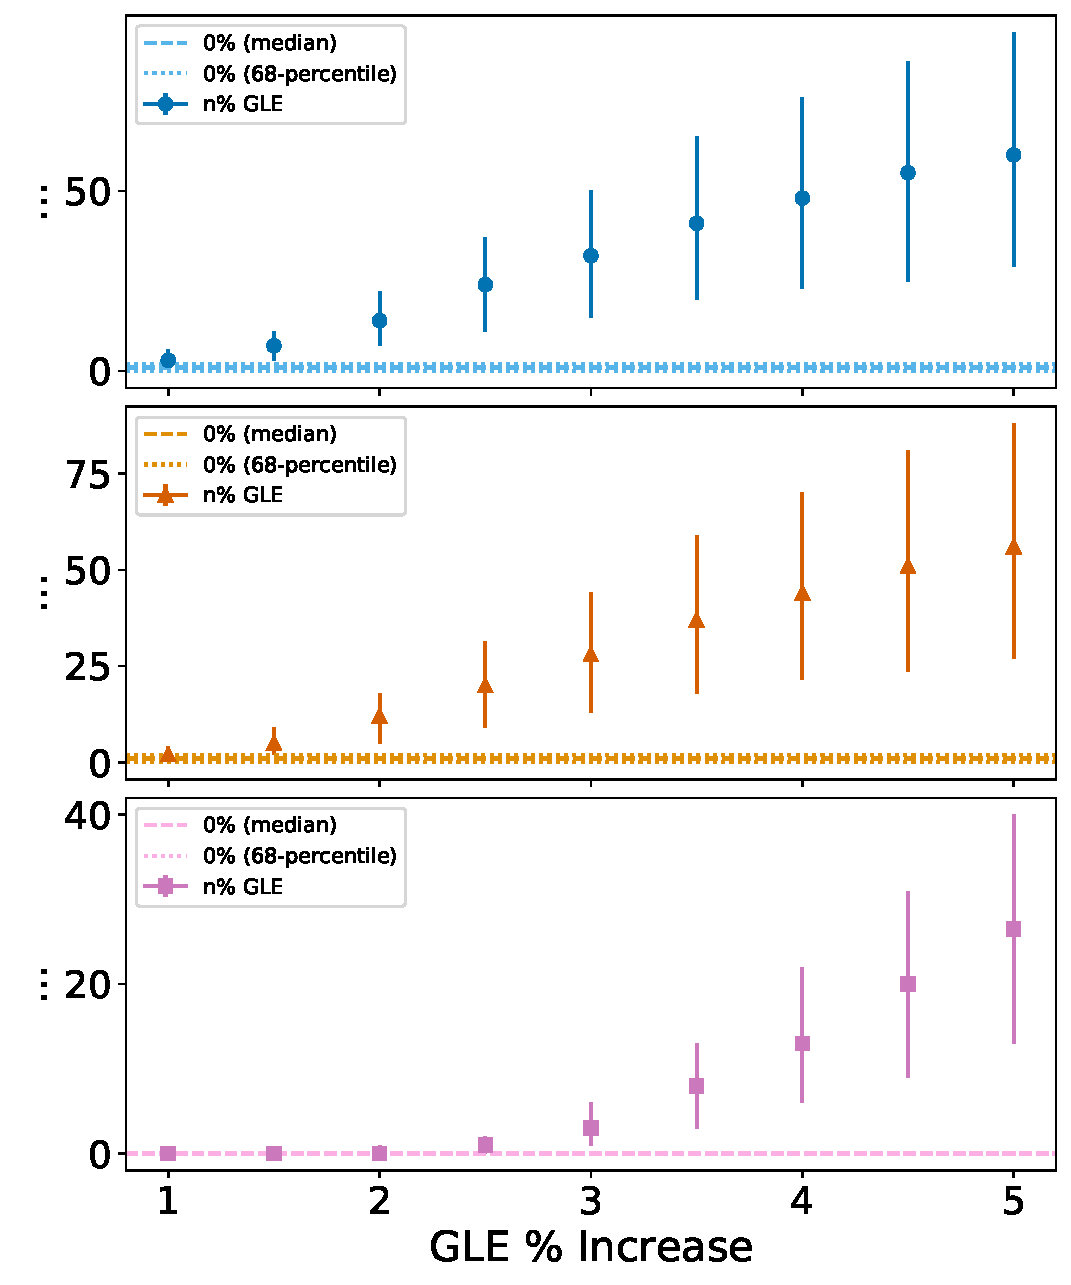
\includegraphics[width=0.48\columnwidth]{HS_14008_sims_plot_5rebin.pdf}
		\label{fig:single_sims_5min_rebin}} \\
	
	\caption{Summary plots showing the number of excessive measurements using the binomial- and Z-tests on the simulations of artificial data with varying magnitudes of GLEs injected. (a) Shows the results for the 10-s cadence data; (b) 1-minute averaged data; (c) 5-minute averaged data. In each plot, the top panel shows the number of significant points exceeding the binomial $p = 10 \%$ threshold, the middle panel shows the number of points exceeding the Z=3 threshold, and the bottom panel shows the number of points exceeding the Z=5 threshold. In each panel the dashed, horizontal lines show the median values of the tests without an injected GLE, and the horizontal, dotted lines represent the $68 \%$ credible intervals either side of the median. For each simulated GLE magnitude the point represents the median values and the error bars represent the $68 \%$ credible intervals either side of the median.}
	\label{fig:single_HS14008_sims}
\end{figure}

We see from Figure~\ref{fig:single_HS14008_sims} that in the case where no averaging of data was performed, using the $Z=3$ significance level, we begin to be able to differentiate the increase in the number of excessive measurements from simply statistical fluctuations for a \gls{gle} with magnitude of $>3.0$--$3.5~\%$. However, in the $Z=3$ test we cannot claim to have observed a statistically significant event (i.e. to $5\sigma$) until a \gls{gle} with magnitude of $\lesssim4.0$--$5.0~\%$. Using the binomial test, we expect to be able to differentiate the increase in the number of significant measurements for a \gls{gle} with magnitude of $>4.5$--$5.0~\%$. To be able to see the results clearly, we only show the results for \gls{gle} magnitudes of up to $5~\%$, and in Figure~\ref{fig:single_sims_0min_rebin}, we see using the $Z=5$ significance level, there are no excessive measurements. In our complete analysis, we investigated \gls{gle} magnitudes up to $10~\%$, and determined that at the $Z=5$ significance level we can differentiate the increase in the number of excessive events for \gls{gle} magnitude of $\geq7.5~\%$. These limiting magnitudes are larger than typical magnitudes of \glspl{gle} predicted in Section~\ref{sec:MAIRE_flux}, hence showing that despite reducing non-\gls{cr} variations in the data, we are only capable of detecting the largest \glspl{gle} in the raw data acquired in this configuration.

When averaging the data over 1-minute and 5-minute intervals, our ability to detect lower-magnitude \glspl{gle} improved. We can differentiate \glspl{gle} from statistical fluctuations for magnitudes of $2.0$--$2.5~\%$ and $\sim1.5~\%$, for 1-minute and 5-minute averaging, respectively. Similarly, at the $Z=5$ significance level this improved to $4.5$--$5.0~\%$ and $2.5$--$3.0~\%$, respectively. Finally, using the binomial test, we expect to be able to differentiate the increase in the number of excessive measurements for a \gls{gle} with magnitude of $\sim2.5~\%$ and $\sim1.5~\%$, respectively.

We also note that with an increasing \gls{gle} magnitude we observe a larger spread in the average number of excessive points. This arises due to the random sampling of \gls{gle} properties, i.e. randomly sampling the rise and decay times. A \gls{gle} with a longer decay time generally results in a higher number of excessive points, compared to a \gls{gle} with a shorter decay time. This effect can be amplified when the magnitude of the \gls{gle} increases as the signal is more statistically significant. Therefore, we see an increase in the confidence intervals for larger \gls{gle} magnitudes in Figure~\ref{fig:single_HS14008_sims}.


This shows that through averaging the data, we expect, with a single detector, that we should be able to detect a \gls{gle} which induces an increase in the muon count rate on the order of $1.5$--$2~\%$. Weighing the benefits of the increased sensitivity against the timescales observable, we recommend making use of the 1-minute averaged data rather than 5-minutes, as the durations of some space weather events can be short-lived, which makes it advantageous to not to average over an ephemeral signal; however, there is added benefit in also analysing the 5-minute averaged data, so a combination of all would be useful. In particular, the interactive \gls{gle} database tends to show data averaged over 5-minutes \citep{usoskin_database_2016}.

Overall, based on the values predicted in Section~\ref{sec:MAIRE_flux}, we believe that it would have been possible to observe the increase in the muon count rate due to \gls{gle} 42, 43, and 45 with this new configuration. We have shown with the raw data we should be able to differentiate a \gls{gle} with magnitude $>3.0$--$3.5~\%$ (i.e. \gls{gle} 42) and when averaging the data into 5-minute bins, we expect to be able to observe \glspl{gle} with magnitudes $> 1.5 \%$  (i.e. \gls{gle} 43 and 45). 


%%%%%%%%%%%%%%%%%%%%%%%%%%%%%%%%%%%%%%%%%%%%%%%%%%%%%%%%%%%%%%%%%%%%%
\subsection{Multiple Station Space Weather Uses}\label{sec:HS_14008_multi_sims}


Many ground-based \gls{cr} detectors typically exist as part of a network, which work together to increase their combined sensitivity. With an increasing number of stations in a network, observing the same events, the combined sensitivity increases by a factor of $\sqrt{N}$, where $N$ is the number of stations in the network, due to the reduction in the Gaussian noise (although, of course, this is limited by the physical limitations of the detectors). However, it is also possible to use other methods to increase the sensitivity of the network and claim observations.

In this section we again use simulations of artificial data (see Appendix~\ref{app:GLE_sims} for details) to determine the magnitude of \glspl{gle} that may be observed with a network of detectors using this configuration. One overarching assumption in this multi-station analysis was that the detectors are all geographically close, such that all the stations are triggered by the \gls{gle} at the same time, or the delay between the signals measured by individual detectors is negligible. We know this assumption is acceptable, based on the coincidental triggering of stations located across the world in the \gls{gnmn} \citep{mishev_current_2020}. In addition, we assumed that all the stations had similar observing properties, as defined earlier. These assumptions are further supported if, for instance, we assume that we upgrade the \gls{hisparc} stations closest to the University of Birmingham. There are another five operational stations in Birmingham which are located within a radius of $<6$~km from this new configuration, and a sixth station within a radius of $\sim$15~km from University of Birmingham. With the exception of the existing University of Birmingham station 14001, which is a 4-detector station, each of the other stations in the Birmingham node have 2-detectors. This means that there are in total an additional 14 individual detectors in the Birmingham node which could be modified into this new configuration.

For each \gls{gle} magnitude we ran 1000 iterations of the simulations and were able to average over the number of excessive measurements for a given \gls{gle} magnitude. The \glspl{gle} were simulated with amplitudes of: $1.0\%$--$5.0\%$; the start times, rise and decay times were all randomly sampled. This was done for 2-, 5-, and 10-stations. In each case we were able to perform the statistics tests on the mean of the data from all stations simulated. Table~\ref{tab:HS_14008_multi_sims_zeros} shows the average number of measurements exceeding the various thresholds for simulations without an injected \gls{gle}.

\vspace{1em}

\begin{table}[ht!]
	\begin{center}
		\caption{Median number of excessive measurements in the mean of the artificial data for multiple stations, with no injected GLEs. The values were acquired from 1000 iterations of simulated data, performing each of the three statistical tests: binomial, $Z=3$, and $Z=5$, with 1, 2, 5, and 10 stations. All uncertainties correspond to the 68\% credible intervals either side of the median.}
		\label{tab:HS_14008_multi_sims_zeros}
		\begin{tabular}{c c c c}
			\hline 
			{} & \multicolumn{3}{c}{\bf No. excessive measurements} \\ 
			{\bf No. stations} & {\bf Binomial} & {\bf $\mathbf{Z=3}$} & {\bf $\mathbf{Z=5}$}  \\ 
			\hline 
			1 & $ 2^{+2}_{-1} $ & $ 27^{+6}_{-5} $ & $ 0 \pm 0 $ \\ 
			2 & $ 3^{+3}_{-2} $ & $ 26^{+26}_{-13} $ & $ 0 \pm 0 $ \\ 
			5 & $ 2^{+4}_{-2} $ & $ 24^{+30}_{-14} $ & $ 0 \pm 0 $ \\ 
			10 & $ 2^{+3}_{-2} $ & $ 24^{+32}_{-15} $ & $ 0 \pm 0 $ \\ 
			\hline 
		\end{tabular} 
	\end{center}
\end{table}
%
%1 & $ 2^{+2}_{-1} $ & $ 27^{+6}_{-5} $ & $ 0 \pm 0 $ \\ 
%2 & $ 2^{+3}_{-1} $ & $ 26^{+22}_{-14} $ & $ 0 \pm 0 $ \\ 
%5 & $ 2^{+4}_{-2} $ & $ 25^{+23}_{-15} $ & $ 0 \pm 0 $ \\ 
%10 & $ 2^{+3}_{-2} $ & $ 25^{+32}_{-16} $ & $ 0 \pm 0 $ \\ 
%

To summarise the results of all the simulations, Figure~\ref{fig:multi_HS14008_sims} shows the average number of excessive measurements against the simulated \gls{gle} magnitude for the 10-s cadence observations, for 1, 2, 5, and 10 stations. % The horizontal, dashed lines shows the median number of statistical fluctuations, i.e. the data in Table~\ref{tab:HS_14008_multi_sims_zeros}; the horizontal, dotted lines represent the $68 \%$ credible intervals. Each point shows the median number of excessive measurements for different \gls{gle} magnitudes, with error bars representing the $68 \%$ credible intervals.


\begin{figure}[!htbp!]
	\centering
	\subfloat[1 station]{
		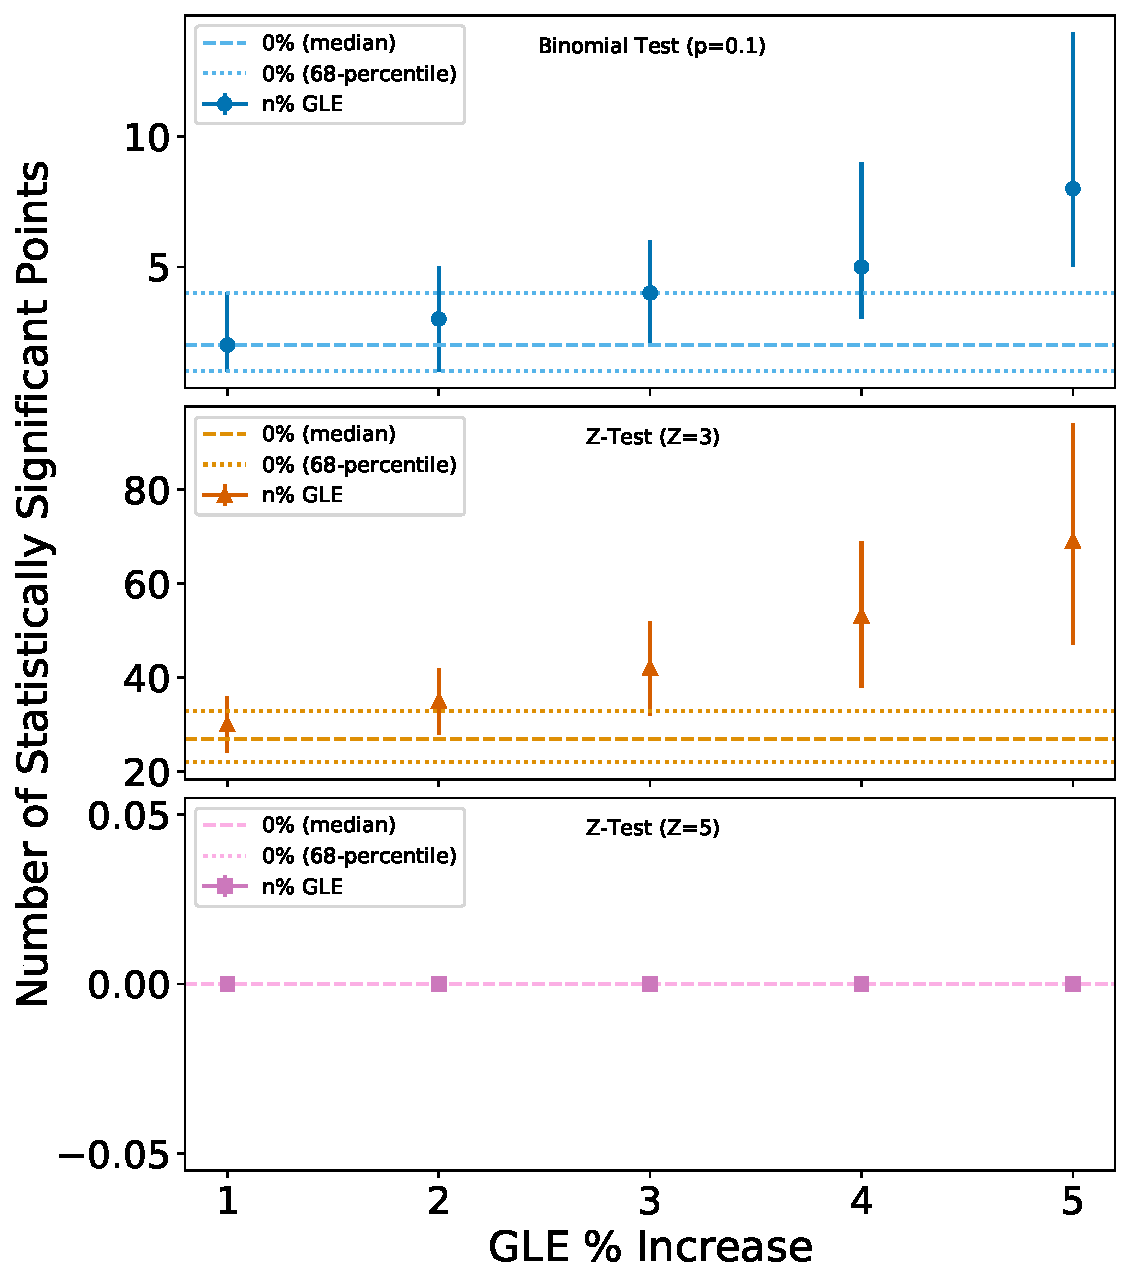
\includegraphics[width=0.48\columnwidth]{HS_14008_sims_plot_1stn.pdf}
		\label{fig:multi_sims_1stn}}
	%\qquad
	\subfloat[2 stations]{
		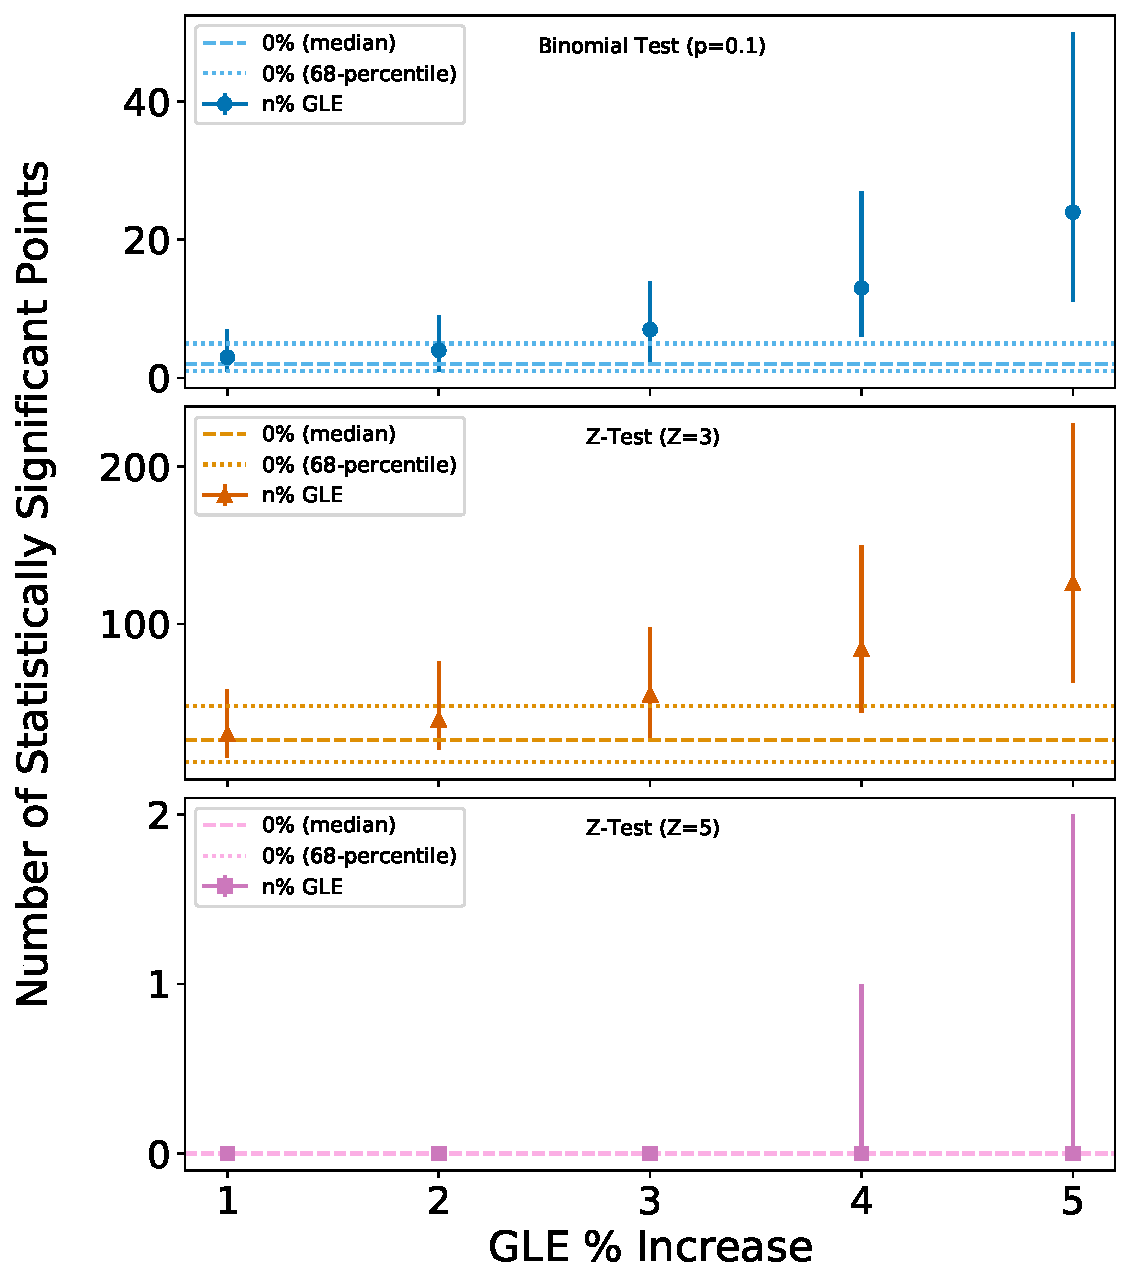
\includegraphics[width=0.48\columnwidth]{HS_14008_sims_plot_2stn.pdf}
		\label{fig:multi_sims_2stn}} \\
	%\qquad
	\subfloat[5 stations]{
		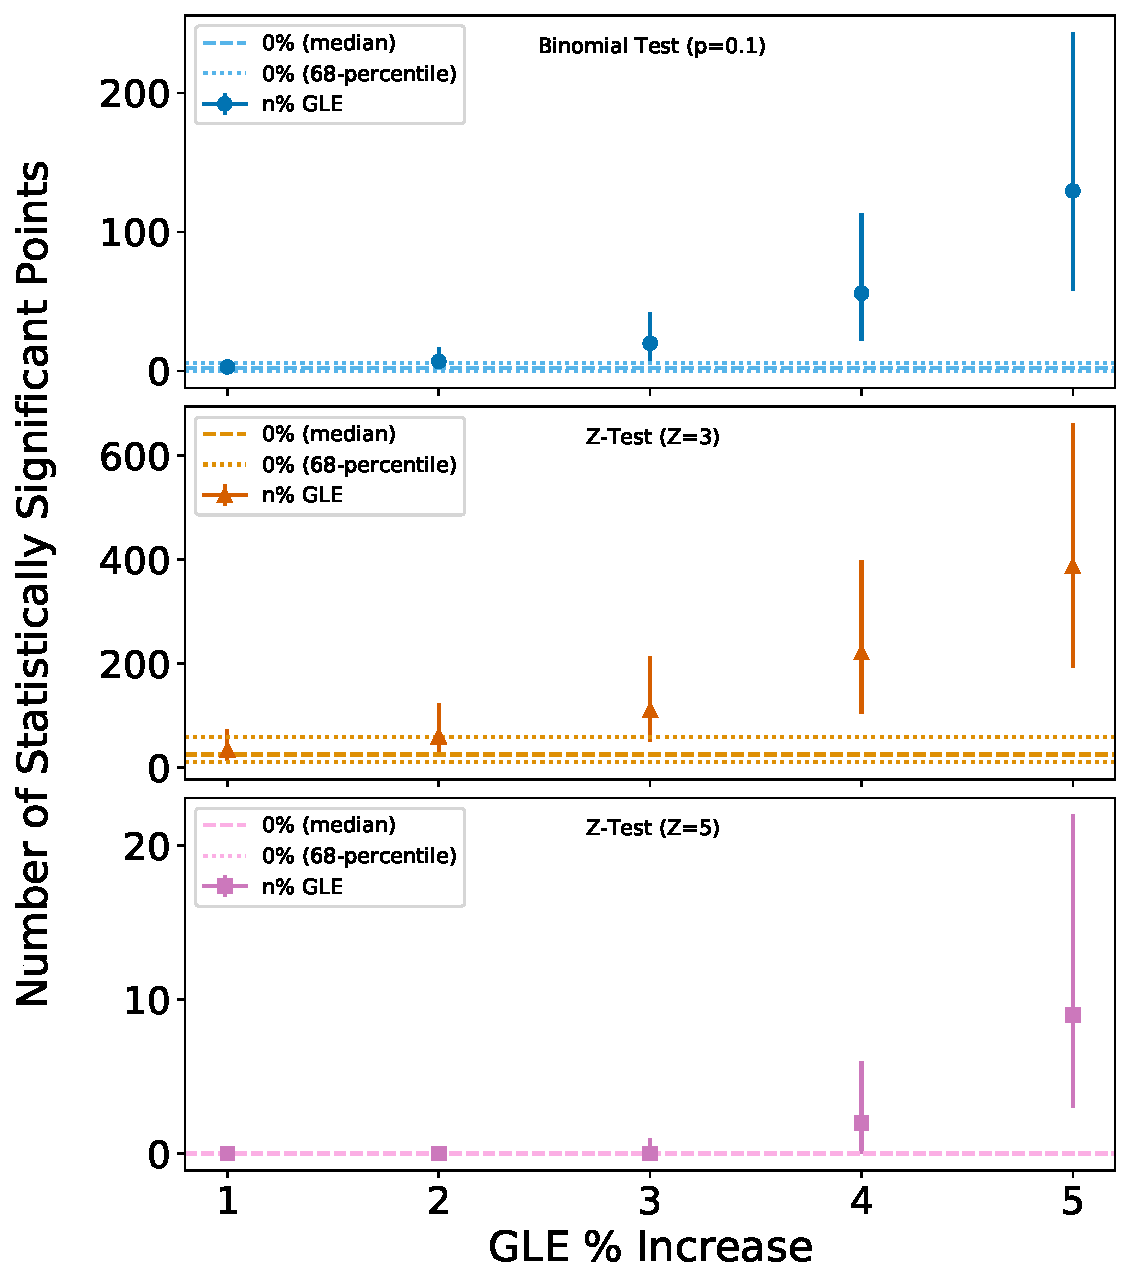
\includegraphics[width=0.48\columnwidth]{HS_14008_sims_plot_5stn.pdf}
		\label{fig:multi_sims_5stn}} 
		%\qquad
	\subfloat[10 stations]{
		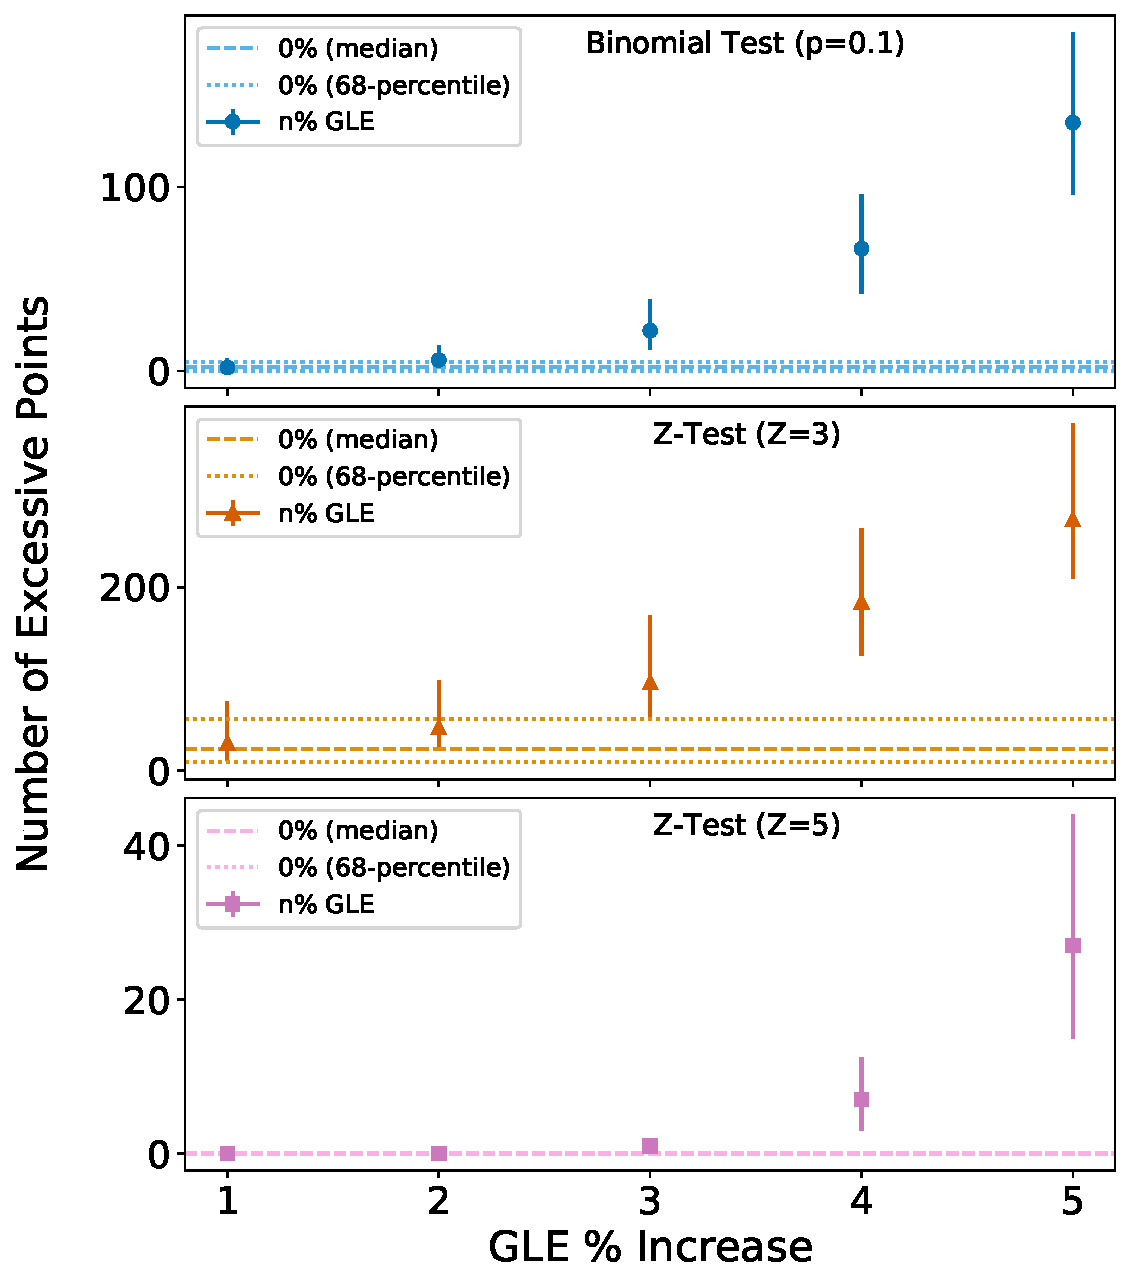
\includegraphics[width=0.48\columnwidth]{HS_14008_sims_plot_10stn.pdf}
		\label{fig:multi_sims_10stn}} \\
	
	\caption{Summary plots showing the number of excessive measurements using the binomial- and Z-tests on the simulations of artificial data with varying magnitudes of GLEs injected. (a) Shows the results for a single station; (b) 2 stations; (c) 5 stations; (d) 10 stations. In each plot, the top panel shows the number of excessive points exceeding the binomial $p = 10 \%$ threshold, the middle panel shows the number of points exceeding the Z=3 threshold, and the bottom panel shows the number of points exceeding the Z=5 threshold. In each panel the dashed, horizontal lines show the median values of the tests without an injected GLE, and the horizontal, dotted lines represent the $68 \%$ credible intervals either side of the median. For each simulated GLE magnitude the point represents the median values and the error bars represent the $68 \%$ credible intervals either side of the median.}
	\label{fig:multi_HS14008_sims}
\end{figure}

We see from Figure~\ref{fig:multi_HS14008_sims} that our ability to differentiate the number of excessive measurements for a \gls{gle} improves with a larger number of stations used. For a single station, using the binomial $10 \%$ threshold, we expect to be able to differentiate the increase in the number of excessive measurements for a \gls{gle} with magnitude of $>4.0$--5.0~\%. Increasing the number of stations to 5 and 10 improved the observable \gls{gle} magnitude to $\sim$3.0--4.0~\% and $\sim$2.0--3.0~\%, respectively. In the case of combining 2 stations, we do not see an improvement due to an exasperation of statistical fluctuations. This shows a greater number of stations is necessary.

For a single station above the $Z=3$ significance level, we have shown we are able to differentiate the increase in the number of excessive measurements for a \gls{gle} with magnitude of $\sim$3.0--4.0~\%; however, increasing the number of stations to 2, 5, and 10 did not improve our ability to ability to observe lower magnitude events. Finally, we see using the $Z=5$ significance level, there were no significant observations for magnitudes $\leq 5\%$ when only using a single station. In the multiple station analysis, we see that for 2, 5, and 10 stations this improved and the observable \gls{gle} magnitude reduced to $\sim$5.0~\%, $\sim$4.0--5.0~\%, and $\sim$3.0--4.0~\%, respectively. 

Despite improving the sensitivity with an increasing number of stations, these limiting magnitudes are larger than typical increase in muon count rate due to \glspl{gle} that were shown in Section~\ref{sec:MAIRE_flux}. This again shows that despite reducing non-\gls{cr} variations in the data, we are only capable of detecting the largest \glspl{gle} in the raw data acquired in this configuration when directly interrogating the data.

As in Section~\ref{sec:HS_14008_single_sims}, we again observe that increasing \gls{gle} magnitude increases the spread in the average number of excessive points. This again arises due to the random sampling of \gls{gle} properties, i.e. the rise and decay times, in the simulations leading to an increase in the confidence intervals for larger \gls{gle} magnitudes in Figure~\ref{fig:multi_HS14008_sims}.


In addition to this analysis, we performed cross-correlation analyses between the stations simulated. This also relied on the assumption that the signal registered at each station has minimal delay, such that the peak of the \gls{ccf} is at a time shift of zero. This analysis was performed for simulations of 2-, 5-, and 10-stations, with varying lengths of the \gls{gle} rise and decay. The resultant \gls{ccf} plots are shown in Figure~\ref{fig:HS_14008_2pc_sim_CCFs}, for a $2 \%$ magnitude \gls{gle}. The individual realisations of the \glspl{ccf}, from combinations of pairs of stations, are plotted as black lines, while the red line shows the mean of the realisations.


\begin{figure}[ht!]
	\centering
	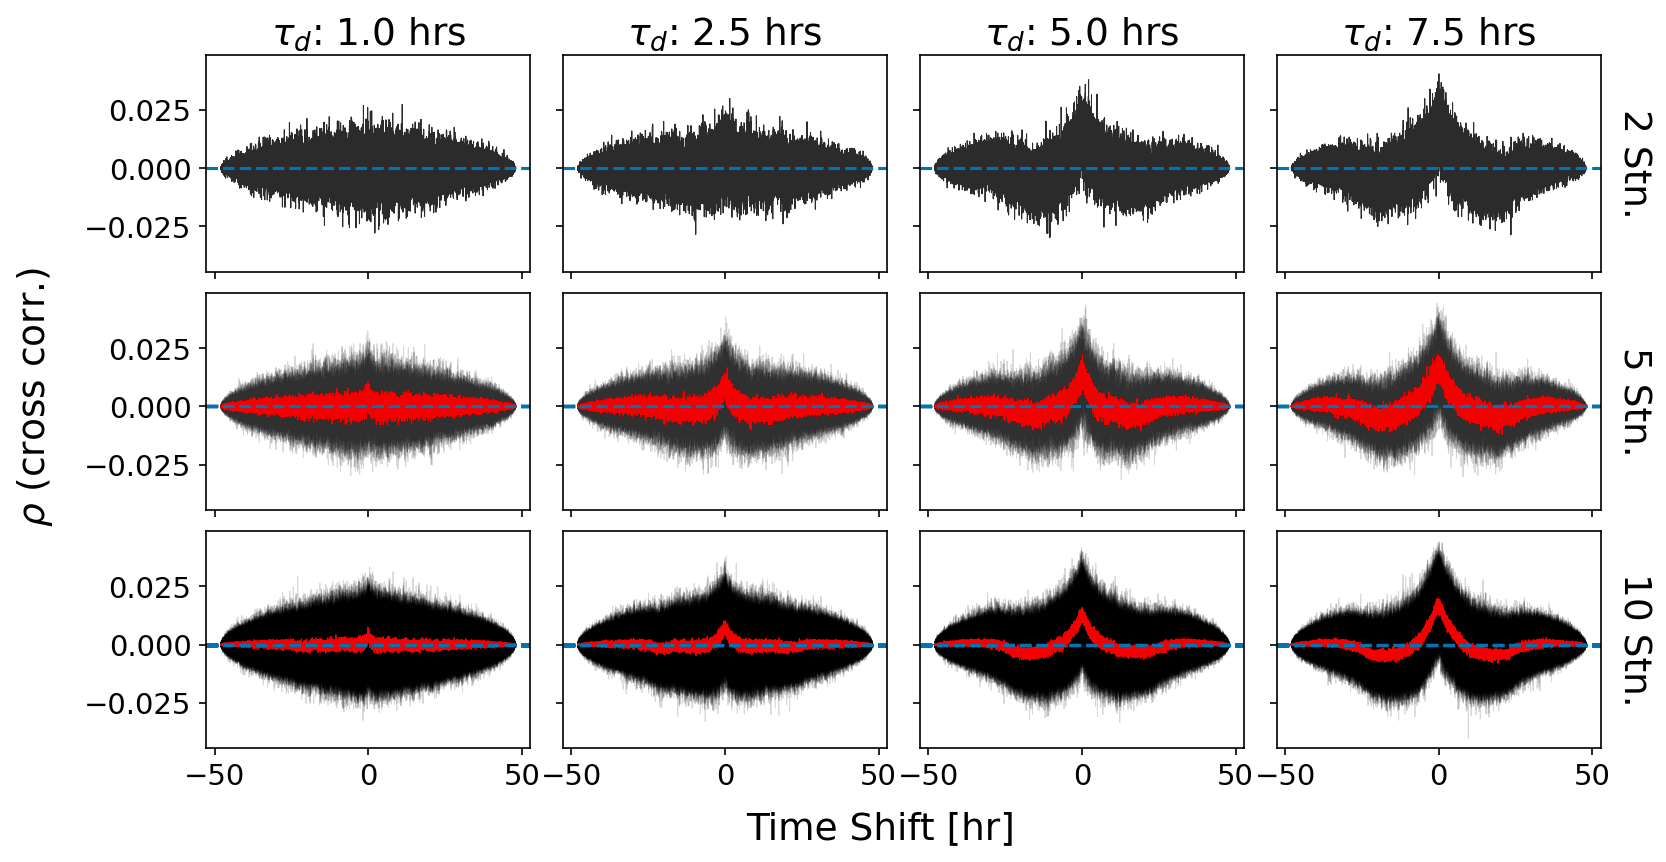
\includegraphics[width=\columnwidth]{HS_14008_sims_CCF_2pc_plot.png}
	\caption{Cross-correlation analyses between 2, 5, and 10 stations for a $2\%$ GLE magnitude with varying rise and decay times. The columns show the results for constant decay times, varying the number of stations, and vice versa for the rows. Black lines show the individual realisations of the CCFs, while the red line shows the mean of all the realisations. Finally, the dashed, horizontal lines depict a correlation of zero.}
	\label{fig:HS_14008_2pc_sim_CCFs}
\end{figure}

As the simulated data all experienced the \gls{gle} at the same time, there was a clear peak in the \gls{ccf} at a time shift of zero hours, as expected, showing a strong asymmetry in the \gls{ccf} around a zero-hour time shift. Assuming that a local network of stations using this configuration also experiences minimal delay between stations, we would expect to observe a similar \gls{ccf} plot, allowing us to claim the detection of a \gls{gle} in each station. Figure~\ref{fig:HS_14008_2pc_sim_CCFs} shows a strong dependence of the length of the \gls{gle} decay on the shape of the \gls{ccf}, with a longer decay providing a clearer, broader \gls{ccf} signal. The average decay time of \glspl{gle} as measured by \citet{strauss_pulse_2017} is $1.8^{+1.9}_{-1.3}$~hours, therefore few \glspl{gle} have decay times $\geq 5$~hours. We should therefore expect that a `typical' \gls{gle} with a similar magnitude would induce a \gls{ccf} with a shape line the first or second columns, i.e. 1.0--2.5~hours. 

We see from Figure~\ref{fig:HS_14008_2pc_sim_CCFs} that increasing the number of stations means we can average over the \glspl{ccf} which results in a less-noisy \gls{ccf}, shown by the red line. In the individual realisations of the \glspl{ccf} (black lines) there is not a significant benefit at this level of \gls{gle} in increasing from 2 to 5 or 10 stations. However, the benefit of an increased number of stations is that we are able to reduce the noise on the combined \gls{ccf} signal. This is advantageous as it allows us to more clearly detect the correlated signals between 5 and 10 stations, versus with only 2 stations. For the simulation using two stations and a decay time of 1~hour in Figure~\ref{fig:HS_14008_2pc_sim_CCFs}, it is difficult to determine a peak near zero-hour time shift, but increasing to 5 and 10 stations shows the benefit, as in the mean \gls{ccf} we then see the peak at a zero-hour time shift. 

This analysis was repeated for simulations of a $1~\%$ \gls{gle}, to investigate whether the increased number of stations allow us to observe \glspl{gle} with such a low magnitude. The results are shown in Figure~\ref{fig:HS_14008_1pc_sim_CCFs}.


\begin{figure}[ht!]
	\centering
	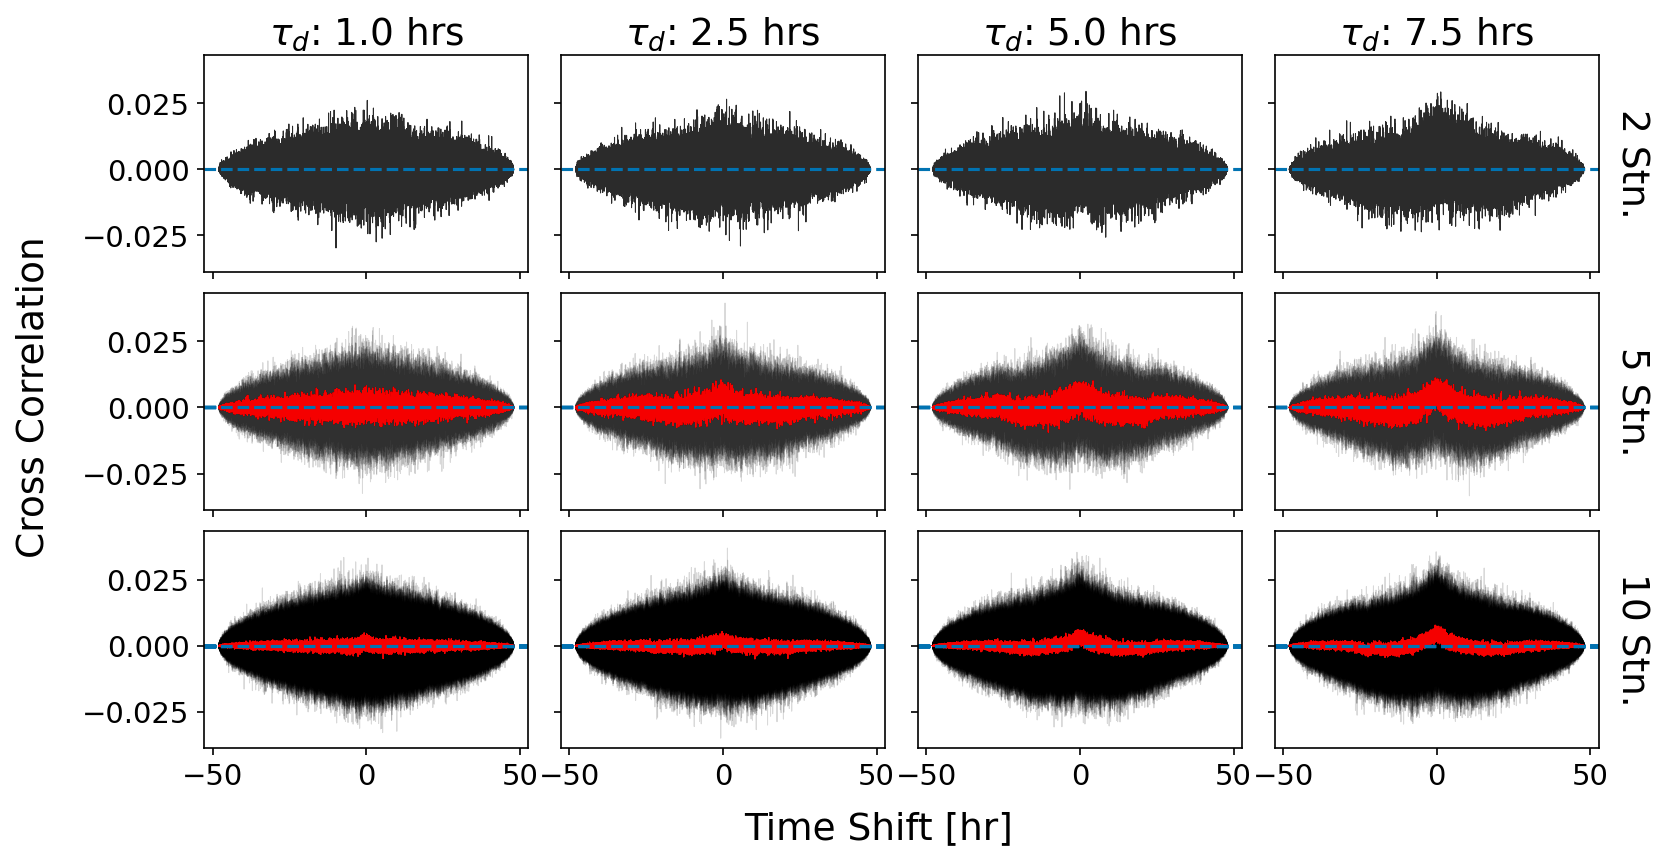
\includegraphics[width=\columnwidth]{HS_14008_sims_CCF_1pc_plot.png}
	\caption{Cross-correlation analyses between 2, 5, and 10 stations for a $1 \%$ GLE magnitude with varying rise and decay times. The columns show the results for constant decay times, varying the number of stations, and vice versa for the rows. Black lines show the individual realisations of the CCFs, while the red line shows the mean of all the realisations. Finally, the dashed, horizontal lines depict a correlation of zero.}
	\label{fig:HS_14008_1pc_sim_CCFs}
\end{figure}


With a $1~\%$ \gls{gle} magnitude it becomes even harder to determine the zero-hour peak. For the simulations with a decay time of 1~hour in Figure~\ref{fig:HS_14008_1pc_sim_CCFs}, it is difficult to determine any peak near zero-hour time shift for the case with 2 and 5 stations and it becomes only slightly visible when increasing to 10 stations. On the other hand, for a decay time of 7.5~hours we can clearly see the \gls{ccf} shape with a peak at zero hours in all cases, i.e. using 2-, 5-, and 10- stations, but we know the average \gls{gle} decay time is closer to 2~hours \citep{strauss_pulse_2017}. At the 2.5~hour decay scale we see the peak in both the 5- and 10-station \glspl{ccf} is observable. Figure~\ref{fig:HS_14008_1pc_sim_CCFs} therefore shows us that at the $1~\%$ \gls{gle} scale, we should sensibly increase the network to 5- or 10-stations to ensure the best chance of observing the cross-correlation in the mean \gls{ccf}.

We generally expect the magnitude of the muon increase due to \glspl{gle} is on the order of or less than $\sim$1~\%, based on the results shown in Section~\ref{sec:MAIRE_flux}. We have shown that we do not expect to observe \glspl{gle} with a single \gls{hisparc} \gls{md}.  We therefore recommend here that any upgrades to form a network should ideally use 10 stations and no fewer than 5 stations, in order to be able to resolve the cross-correlation between the stations. % In addition, the average decay time of \glspl{gle}, as measured by \citet{strauss_pulse_2017}, is $1.8^{+1.9}_{-1.3}$~hours.


%%%%%%%%%%%%%%%%%%%%%%%%%%%%%%%%%%%%%%%%%%%%%%%%%%%%%%%%%%%%%%%%%%%%%
%%%%%%%%%%%%%%%%%%%%%%%%%%%%%%%%%%%%%%%%%%%%%%%%%%%%%%%%%%%%%%%%%%%%%
\section{Conclusions}\label{sec:HS_14008_conclusion}

In this chapter we have presented a new \gls{hisparc} station configuration and investigated its performance for use monitoring space weather events. We have outlined the set-up of the new station, from the configuration of the scintillators, calibration of the \glspl{pmt}, processing of the \gls{pmt} signals using a series of \gls{nim} modules, and the acquisition of data using a Raspberry Pi. We have also outlined how we acquire atmospheric pressure data and the temperature measured within the roof box. Both measurements were used to correct for effects on the acquired \gls{cr} data.

The station was configured to collect two types of coincidence data: (i) the full coincidence counts between the two \glspl{pmt}; (ii) a reduced coincidence count, which is between the original coincidences and a gate signal. The reduced count rate was necessary to not overload the \gls{hisparc} servers.

The removal of the atmospheric effects was routinely performed on the acquired singles and coincidences data. We showed for the coincidences data it was only necessary to correct for the effects of pressure. The configuration of the station uses the coincident signal from two separate \glspl{pmt} and we showed there was only a weak correlation with temperature which was likely due to the diurnal \gls{cr} anisotropy rather than temperature. This was further supported in our investigation of the spurious counts, when investigating the noise in the coincidences data, which did not show a diurnal signal. The temperature correction was however still necessary for singles data and we demonstrated the success of this method. In both data it was necessary to correct for atmospheric pressure, which we showed was successful when using pressure data measured  $\sim$20~km from this \gls{hisparc} station.

After atmospheric corrections, we analysed the coincidences data by using a Poisson likelihood function to determine the posterior distribution for the mean of the count rate. In addition, it was demonstrated by adding a large delay between the two \glspl{pmt} that we were able to quantify the noise (spurious counts) in the coincidences data, caused by random coincidences between the two \glspl{pmt}. As discussed above, this noise did not show any diurnal variation, meaning the diurnal temperature effects in the singles data did not bleed through into the coincidences data. Through the analysis of the original and reduced coincidences data, we were able to quantify the reduction factor, which was as expected from the duty cycle of the gate signal and we showed that there is agreement between the reduced data stored locally and that stored on the \gls{hisparc} servers, with only differences being realisations of the Poisson noise.

A further study was conducted to understand the magnitudes of \glspl{gle} that should be observable with this new configuration. This used simulation of artificial data and we were able to perform statistical tests, comparing the number of statistically significant measurements in 2~days of data with \glspl{gle} of varying magnitude. We showed this method was suitable for claiming observations of \glspl{gle} and showed that through averaging the data over 1- and 5-minutes, we can reduce the noise to observe lower \gls{gle} magnitudes.

Expanding on this, we also performed analyses using artificial data with multiple stations. This was done to examine whether upgrading to a network of several \gls{hisparc} stations in this configuration would improve our ability to observe low-magnitude \glspl{gle}. We performed statistical tests on the mean signal between the stations and also performed cross correlation analyses. We demonstrated that there exists a strong dependence on the decay time of the \gls{gle} on the shape of the \gls{ccf} signal, but increasing the number of stations allowed us to observe the correlation.


We leave the reader with the following points:

\begin{enumerate}
	\item{A new configuration of \gls{hisparc} detector has been implemented, which is more relevant for space weather applications, as it overcomes the bias towards higher energy \glspl{pcr} that the \gls{hisparc} experiment intends to observe. It also reduces the atmosphere induced diurnal effects.}%, which are difficult to correct in the data from the existing \gls{hisparc} stations.}

	\item{The mean count rate in this configuration is $\sim$80~$\upmu/\mathrm{s}$ and the noise from spurious counts is of about $0.0043\pm0.0002~\upmu/\mathrm{s}$. This noise is small and negligible compared to the Poisson noise of $\sim$9~$\upmu/\mathrm{s}$, which represents $\sim$11~\% of the signal. The reduced coincidences data has a count rate which is lower by a factor of approximately 110, and the reduced counts data has been shown to be in agreement for the data stored locally and that stored in the \gls{hisparc} servers.}
	
	\item{There exists a good visual agreement between the data monitored by this station and a local \gls{nm} station, Dourbes, in Belgium. The data from this station and from the Dourbes \gls{nm} station should be continually compared to monitor this relationship, as it will be instrumental when or if a space weather event occurs in the next Solar Cycle.}
	
	\item{Simulations of artificial data demonstrated that with the raw, 10-s cadence observations we should expect to be able to detect \glspl{gle} with this configuration with a magnitude of $\gtrsim3$--4~\%. Through averaging the data into 1- or 5-minute bins, we reduce the noise and improve the sensitivity to observe \glspl{gle} with magnitudes $\gtrsim1.5$--2.0~\%. This is in line with some of the predicted \gls{gle} magnitudes from Chapter~\ref{chap:HiSPARC}.}
	
	\item{Through simulating the performance of a network of detectors in this configuration we showed that we can improve the sensitivity, to observe \glspl{gle} on the order of $\sim$1~\%, through analysing the cross-correlation of nearby stations. However, we note that there is a strong dependence on decay time of the \glspl{gle}. We recommend that any upgrades to form a network should ideally use 10 stations and no fewer than 5 stations.}
	
	\item{It is important that this configuration of \gls{hisparc} detector is maintained until at least 2026, to ensure a complete study is performed to at least the maximum of Solar Cycle 25.}
\end{enumerate}